% ------------------------------------------------------------------------
% ------------------------------------------------------------------------
% abnTeX2: Modelo de Trabalho Acadêmico (tese de doutorado, dissertação de
% mestrado e trabalhos monográficos em geral) em conformidade com 
% as normas da ABNT
% ------------------------------------------------------------------------
% ------------------------------------------------------------------------

\documentclass{dcomp-abntex2}

% Geração de dummy text
% Retirar para a versão final do documento
\usepackage{lipsum}
\usepackage{amsmath}
\usepackage{graphicx}
%Compila o indice
\makeindex

\begin{document}

% Seleciona o idioma do documento (conforme pacotes do babel)
\selectlanguage{brazil}

% Retira espaço extra obsoleto entre as frases.
\frenchspacing 

% ----------------------------------------------------------
% ELEMENTOS PRÉ-TEXTUAIS
% ----------------------------------------------------------
\pretextual

\titulo{Modelagem 3D de ambientes através de câmeras}
\autor{Guilherme Gomes Cardoso\\
	Ítalo Lessa Oliveira}
\orientador{Prof. Dr. Daniel Oliveira Dantas}
\curso{Ciência da Computação}

\imprimircapa
\imprimirfolhaderosto*

%\imprimirfichacatalografica
%\imprimirfolhadeaprovacao	
    
\begin{dedicatoria}
   \vspace*{\fill}
   \centering
   \noindent
   \textit{} \vspace*{\fill}
\end{dedicatoria}
% ---
\begin{agradecimentos}
Os agradecimentos principais são direcionados à Gerald Weber, Miguel Frasson,
Leslie H. Watter, Bruno Parente Lima, Flávio de Vasconcellos Corrêa, Otavio Real
Salvador, Renato Machnievscz\footnote{Os nomes dos integrantes do primeiro
projeto abn\TeX\ foram extraídos de
\url{http://codigolivre.org.br/projects/abntex/}} e todos aqueles que
contribuíram para que a produção de trabalhos acadêmicos conforme
as normas ABNT com \LaTeX\ fosse possível.

Agradecimentos especiais são direcionados ao Centro de Pesquisa em Arquitetura
da Informação\footnote{\url{http://www.cpai.unb.br/}} da Universidade de
Brasília (CPAI), ao grupo de usuários
\emph{latex-br}\footnote{\url{http://groups.google.com/group/latex-br}} e aos
novos voluntários do grupo
\emph{\abnTeX}\footnote{\url{http://groups.google.com/group/abntex2} e
\url{http://www.abntex.net.br/}}~que contribuíram e que ainda
contribuirão para a evolução do \abnTeX.

\end{agradecimentos}
% ---
\begin{epigrafe}
    \vspace*{\fill}
	\begin{flushright}
		\textit{ “I came seeking a challenge. All i found was you.”\\
   (Zurgo Helmsmasher, to Narset)} \vspace*{\fill}
   
      \textit{ “Some convictions are so strong that the world must break to accomodate them”\\
   (texto da carta Vindicate)} \vspace*{\fill}
	\end{flushright}
\end{epigrafe}
% ---
% resumo em português
\setlength{\absparsep}{18pt} % ajusta o espaçamento dos parágrafos do resumo
\begin{resumo}
A reconstrução 3D de ambientes vêm sendo utilizada em diversos campos, como por exemplo: O mapeamento de ambientes para pesquisa arqueológica em áreas onde os cientistas não podem alcançar, ou comparar uma área antes e depois de uma catástrofe\cite{SLAMAP}, também em automação de robôs para que eles possam se locomover em um ambiente e agora, um dos mais recentes usos é a realidade virtual para jogos. Infelizmente, ainda há certas limitações, pois a câmera utilizada influencia imensamente no resultado (além do fato de que precisa estar devidamente calibrada). Normalmente para o mapeamento, são utilizadas várias câmeras, para obter diversos pontos de vista para um mesmo objeto (semelhante à como os olhos humanos percebem o ambiente), e há técnicas e procedimentos para realizar o mapeamento com apenas uma câmera com a ajuda da \textit{Multiple View Geometry}. O objetivo deste trabalho é utilizar tais fundamentos para obter a reconstrução do ambiente, inicialmente de um \textit{smartphone}, resultando no aplicativo PhotoGuide. Tal aplicativo reconhece keypoints de um vídeo ou diretamente da câmera, mas por problemas de desempenho, foi necessário mover o processamento para máquinas mais poderosas, como um \textit{desktop} trocando a ferramenta de reconstrução para o \textit{LSD-SLAM}, que fornece um pacote completo de ferramentas para reconstruções 3D. 

 \textbf{Palavras-chave}: Reconstrução 3D. LSD-SLAM. Processamento de imagens. Mapeamento do Ambiente.

\end{resumo}
% resumo em inglês
\setlength{\absparsep}{18pt} % ajusta o espaçamento dos parágrafos do resumo
\begin{resumo}[Abstract]
\textit{Environment 3D reconstruction has being used in several fields, for example, the environment mapping for archeological research at areas where scientists can't reach, or compare one area before and after a catastrophe\cite{SLAMAP}, also in robot automatization so it can move in an environment and now, one of it most recent uses is virtual reality for games. Unfortunately, it still has some limitations, since the camera used influentiate greatly on the result (besides the fact it must be well calibrated). Usually for mapping, several cameras are used, in order to obtain many point of view for the same object, in a similar fashion as human eyes perceive the environment, and several techniques and procedures exist to realize the mapping with only one camera with the help of Multiple View Geometry. The goal of this work is to use these concepts in order to obtain the reconstruction of an environment, initially using a smartphone, resulting in the PhotoGuide app. That app recognizes keypoints from a video of directly from the camera, but due to performance problems, was needed shift the process to more powerful machines, as a desktop, and change the reconstruction tool to LSD-SLAM, which provides the full suite of 3D reconstruction tools.}

% \end{otherlanguage*}

\textit{\textbf{keywords}: 3D Reconstruction. LSD-SLAM. Images processing. Environment mapping}.
\end{resumo}
    
\pdfbookmark[0]{\listfigurename}{lof}
\listoffigures*
\cleardoublepage

\pdfbookmark[0]{\listtablename}{lot}
\listoftables*
\cleardoublepage
    
% ---
% inserir lista de abreviaturas e siglas
% ---

\begin{siglas}
\item[BRIEF]\textit{Binary Robust Independent Elementary Features}
\item[FAST]\textit{Features from Accelerated Segment Test}
\item[FPS]\textit{Frames Per Second}
\item[GUI]\textit{Graphical User Interface}
\item[JNI]\textit{Java Native Interface}
\item[LSD-SLAM]\textit{Large Scale Direct SLAM} 
\item[OPENCV]\textit{Open Computer Vision}
\item[ORB]\textit{Oriented FAST and Rotated BRIEF}
\item[RAM]\textit{Random Access Memory}
\item[RANSAC]\textit{Random Sample Consensus}
\item[ROS]\textit{Robot Operating System}
<<<<<<< HEAD
\item[SFM]\textit{Structure From Motion}
\item[SIFT]\textit{Scale-Invariant Feature Transform}
\item[SLAM]\textit{Simultaneous Localization And Mapping}
\item[SURF]\textit{Speeded Up Robust Features}
=======
\item[GUI]\textit{Graphical User Interface}
\item[FPS]\textit{Frames Per Second}

>>>>>>> 06125d0733c1f4056ec74812744e571f3532812a
\end{siglas}
% ---
% ---
% inserir lista de símbolos
% ---

\begin{simbolos}
  \item[$ \xi $] Letra grega minúscula ksi
  \item[$ \in $] Pertence
\end{simbolos}
% ---
    
\pdfbookmark[0]{\contentsname}{toc}
\tableofcontents*
\cleardoublepage

% ----------------------------------------------------------
% ELEMENTOS TEXTUAIS
% ----------------------------------------------------------
\textual
\chapter{Introdução}

Apresentaremos neste capítulo a motivação para este trabalho, problemas encontrados e outros trabalhos que também tentam reconstruir ambientes. A forma como o trabalho está estruturado e a sua proposta inicial será apresentada também.

\section{Motivação}

Alguns avanços tecnológicos atualmente são graças à modelagem de ambientes, alguns deles que podem ser citados são: a melhor investigação forense com o mapeamento das cenas de um crime \cite{FIT3D}, o carro autônomo em desenvolvimento pela \textit{Google} \cite{googlex} e realidade virtual, criando assim novos ramos de pesquisa, novos mercados à serem explorados.

Um potencial uso, em que a vida de diversas pessoas seria mudada, é a utilização do mapeamento, seja ele \textit{on the fly} ou realizado a priori, para guiar pessoas com deficiência visual num ambiente. Alguns trabalhos semelhantes foram realizados mas diversas dificuldades foram encontradas. Uma delas é a questão de identificar a forma dos mais diversos objetos e também a topografia do ambiente. 


\section{Objetivos}

Os objetivo deste trabalho é realizar, mesmo que parcialmente, o mapeamento 3D de estruturas e ambientes, internos e externos, a fim de utilizá-lo para outros fins potenciais. Tendo como estudo de caso, a reconstrução 3D do prédio do departamento de computação.

\subsection{Objetivos Específicos}

Para atingir o objetivo, foram utilizadas duas câmeras: uma câmera \textit{USB} do modelo PSEye® e a câmera nativa do smartphone \textit{Motorola Moto X Play 32GB} para obter imagens e vídeos do ambiente; o software \textit{LSD-SLAM} \cite{LSD-SLAM-Artigo} para modelagem e o \textit{software VLC} para extrair os quadros dos vídeos capturados pelas câmeras a fim de criar os \textit{datasets}. Ao longo do trabalho, foi criado um aplicativo para o sistema mobile \textit{Android}, onde é possível calibrar a câmera do dispositivo \textit{smartphone Android} e também gravar os \textit{datasets} necessários para o trabalho, na tentativa de dispensar a necessidade de um computador em todas as partes da obtenção e processamento do \textit{dataset}.


\section{Abordagem utilizada}

O trabalho possui as seguintes fases:
%considerar usar description lista no lugar
\begin{itemize}
\item{Estudo sobre o estado da arte: Foram pesquisados os diversos métodos disponíveis atualmente para mapeamento de ambientes, bem como seus pormenores. Também como  poderiam ser utilizados para o objetivo deste trabalho}
\item{Criação de um aplicativo para o sistema operacional \textit{Android}, onde fosse possível calibrar a câmera e obter um preprocessamento do \textit{dataset}, na forma de um banco de dados com quadros e seus \textit{keypoints}}
\item{Estudo e testes com as ferramentas encontradas: Várias ferramentas para reconstrução de ambientes foram encontradas, e nesta fase todas seriam testadas}
\item{Criação do \textit{dataset}: Vídeos e imagens do ambiente externo e interno do departamento}
\item{Processamento e avaliação do \textit{dataset}: Nesta fase foi realizado o processamento do \textit{dataset} com a ferramenta \textit{LSD-SLAM}, onde foi preciso realizar diversos testes para um melhor refinamento de suas configurações}
\end{itemize}


\section{Estrutura do Documento}


Este trabalho está dividido da seguinte forma: No Capítulo 2 será apresentado o estado da arte sobre reconstrução 3D de ambientes; no Capítulo 3 a metodologia utilizada para obter os objetivos deste trabalho; no Capítulo 4 serão mostrados detalhes da instalação e uso da ferramenta \textit{LSD-SLAM}; no Capítulo 5 serão abordados os resultados obtidos e por fim no Capítulo 6 a conclusão e possíveis trabalhos futuros.



\chapter{Estado da arte}

\section{\textit{Structure from motion}}

\textit{Structure from motion} é o processo de estimar estruturas 3D partindo de imagens sequenciais em duas dimensões \cite{SFM}, que pode conter sinais de movimento, em analogia com a biologia, seria o equivalente ao modo  como os olhos humanos e de outros animais conseguem recuperar estruturas 3D de um plano 2D, nesse caso a retina, partindo de uma cena ou objeto em movimento.

Tendo como exemplo os planos $C$ e $C'$ na equação \eqref{eq1}, dois pontos, chamados $m$ no plano $C$ e $m'$ no plano $C'$, podem ser chamados de correspondentes se há projeções do mesmo ponto 3D no espaço $M$. Havendo mais de uma imagem, algumas perguntas podem ser feitas, como:

\begin{itemize}
	\item{Dado um ponto $m$ na primeira imagem, onde está seu correspondente $m’$ na segunda imagem?}
	\item{Qual a geometria 3D da cena?}
	\item{Qual a posição relativa de ambas câmeras?}
\end{itemize}
	
Com pelo menos duas imagens em diferentes posições, se torna possível inferir a posição 3D de um ponto utilizando sua diferença de posição em ambas imagens. Para tanto é necessário deduzir a posição de duas retas num sistema de coordenadas em comum e é preciso também ter conhecimento da posição relativa da segunda imagem ou câmera com a primeira, o que pode ser chamado de movimento.

Algebricamente, se soubermos as matrizes de projeção $P$ e $P'$, podemos computar $M$ a partir de $m$ e $m'$, resolvendo o sistema linear de 4 equações, três incógnitas abaixo \cite{Faugeras-Geometry}:


\begin{equation}\label{eq1}
\begin{aligned}
	PM = m \\
	P'M = m'
\end{aligned} \; \;
\begin{bmatrix}
		P
\end{bmatrix}_{3x4}	
\underbrace{\begin{bmatrix}
		x \\ y \\ 1
\end{bmatrix}
}_{M}
\underbrace{\begin{bmatrix}
		m\\v\\1
\end{bmatrix}}_{m}	
\underbrace{\begin{bmatrix}
		m'\\v'\\1
	\end{bmatrix}}_{m'}
\end{equation}
 

Equação \eqref{eq1}: Matriz de projeção $P$, plano $M$ e retas $m^T = \begin{bmatrix}u & v & 1\end{bmatrix}$ e $m'^T = \begin{bmatrix}u' & v' & 1\end{bmatrix}$, respectivamente.

\begin{equation}\label{eq2}
\begin{cases}
P M \simeq m, \\
P' M \simeq m'.
\end{cases}
\end{equation}

Equação \eqref{eq2}: Sistema de equações para a matriz de projeção $P$ e $P'$, respectivamente.

Para encontrar a estrutura 3D da cena, é necessário obter as matrizes de projeção $P$ e $P'$, pois possuem informações acerca da geometria da cena. O sistema de equações \eqref{eq2} possui três incógnitas e para que seja possível uma solução, as coordenadas de $m$ e $m'$ precisam satisfazer algumas restrições, logo, o ponto $m'$ não pode ser um ponto arbitrário na segunda imagem.

Seja um exemplo em que os pontos 3D estejam num plano II, havendo uma homografia \cite{Faugeras-Geometry} entre II e cada uma das imagens, pode-se concluir que há uma homografia entre ambas imagens, chamada \textbf{homografia planar}, definida por uma matriz $M$ de tamanho 3x3. A homografia é exemplificada como equação pela equacão \eqref{eq3} e também na figura \ref{fig1}:

\begin{equation}\label{eq3}
m' \simeq Hm.
\end{equation}

Equação \eqref{eq3}: Relação de homografia entre um ponto $m'$ da segunda imagem com um ponto $m$ da primeira, como equação.

\begin{figure}[H]
	\centering
		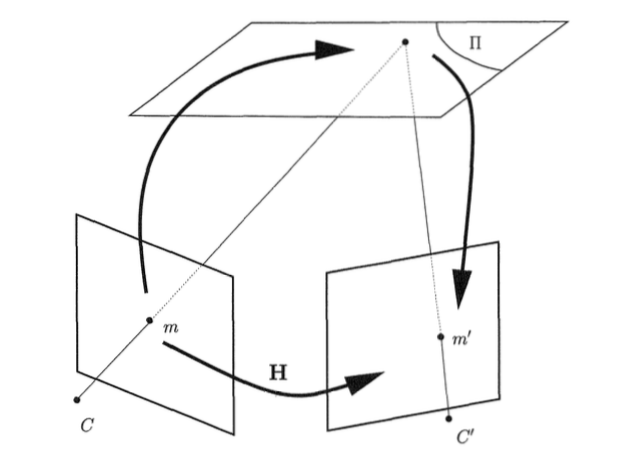
\includegraphics{Imagens/figura2-1.png}
	\caption{Relação de homografia entre um ponto $m'$ da segunda imagem com um ponto $m$ da primeira. Faugeras et al [2] pag. 22.}
	\label{fig1}
\end{figure}

 Sejam $m$ e $m'$ pontos arbitrários da imagem 1 e 2, respectivamente, para qualquer plano II que não passe pelo centro ótico das imagens, as imagens também são pontos de intersecção dos raios em comum de ambas. Portanto, são relacionadas pela matriz $H$. Essa homografia pode ser utilizada para construir mosaicos, como mostra a figura \ref{fig2} acima. Apesar de conseguir gerar um campo de visão maior, não é possível obter coordenadas 3D à partir de imagens com o mesmo centro óptico \cite{Faugeras-Geometry}, pois a ambiguidade continua já que os raios correspondentes são idênticos. Um outro caso que vale frisar é quando os centros ópticos de ambas imagens são o mesmo, como por exemplo, quando tiradas do mesmo ponto mas apenas com uma rotação, também não será possível haver homografia.

\begin{figure}
	\centering
		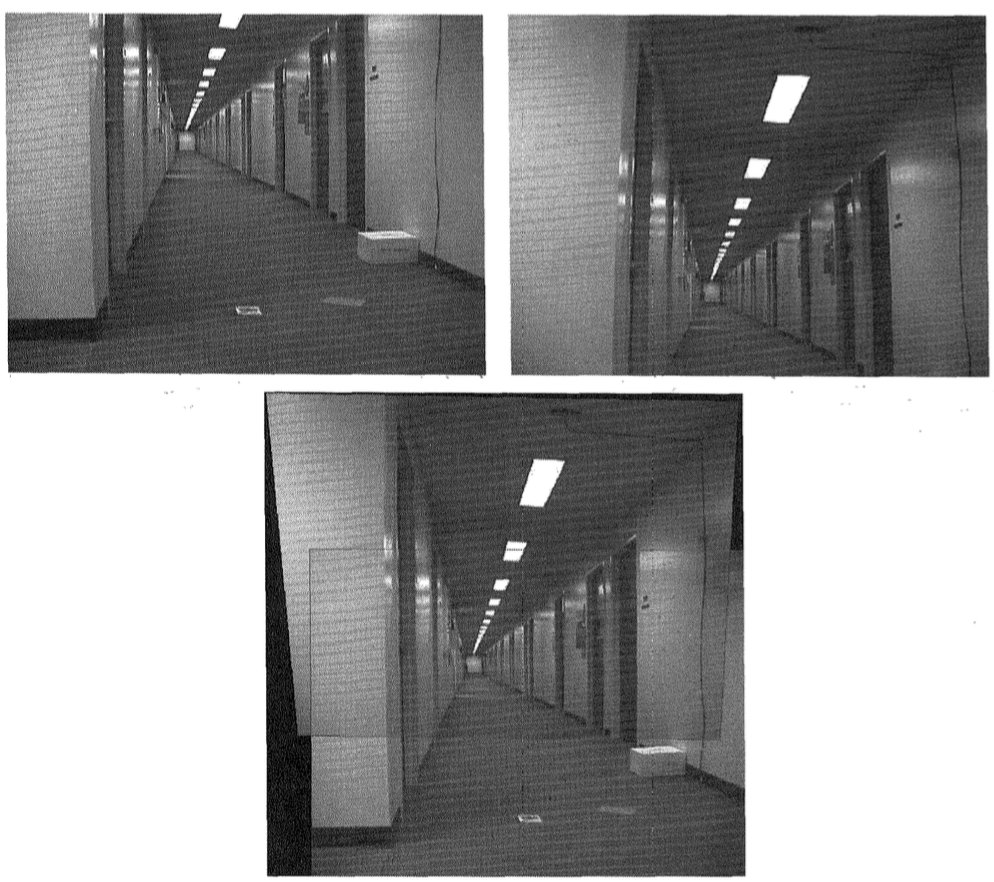
\includegraphics[width=1.0\textwidth]{Imagens/figura2-2.png}
	\caption{Duas imagens obtidas com o mesmo ponto de vista, e a imagem resultante da junção das duas com homografia. Faugeras et al \cite{Faugeras-Geometry} pag. 24.}
	\label{fig2}
\end{figure}

Quando os pontos no espaço e as duas câmeras estão em posições distintas, não é possível predizer a posição do correspondente $m'$ de um ponto qualquer $m$ da primeira imagem, pois essa informação depende da profundidade do ponto 3D ao longo do raio óptico. Geometricamente essa posição não é arbitrária, o ponto $m$ precisa estar numa linha, o raio óptico, logo $m'$ precisa estar localizado na projeção da reta na segunda imagem. Essa linha é chamada \textbf{Linha Epipolar}, do ponto \textbf{m} na segunda imagem. Tendo conhecimento dela, ao procurar o correspondente $m'$, não é necessário procurar em toda a imagem, bastando apenas na linha, reduzindo então uma busca 2D para 1D, mostrado na figura \ref{fig3}.

\begin{figure}
	\centering
		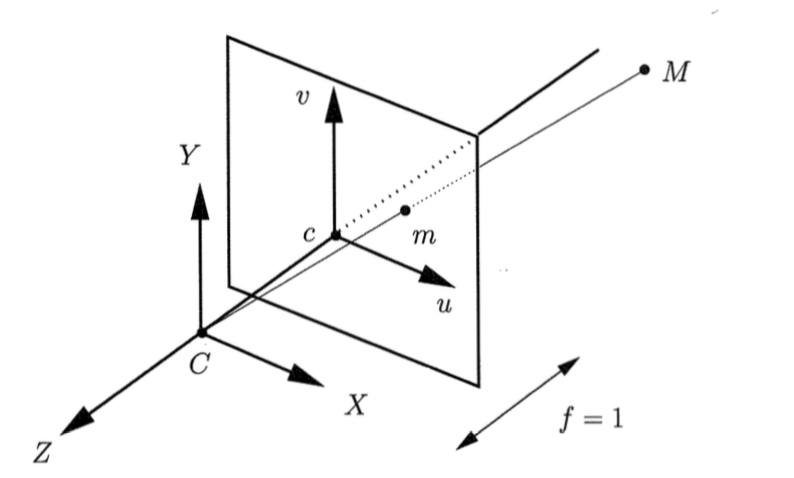
\includegraphics{Imagens/figura2-3.png}
	\caption{Exemplificação da redução de 2D para 1D. Faugeras et al \cite{Faugeras-Geometry} pag. 12.}
	\label{fig3}
\end{figure}

Outra forma de se obter o mesmo resultado é considerar algumas restrições às câmeras ao invés de sua correspondência. Supondo que há uma correspondência válida entre $m$ e $m'$, a posição relativa de ambas as câmeras precisa ser de forma que os raios ópticos $L_{m}$, que cruza o centro óptico da primeira imagem e o ponto $m$, e $L_{m}'$, que cruza o centro óptico da segunda imagem e o ponto $m'$, se interceptem. Algebricamente, já que o ponto $M$ da figura \ref{fig3} depende de três coordenadas, e a correspondência entre $m$ e $m'$ depende no total de 4 parâmetros, é necessário também que haja uma relação algébrica entre as coordenadas de $m$ e $m'$.

A relação entre o ponto $m$ e a linha epipolar $l'_{m}$ na segunda imagem é linearmente projetiva, já que o raio óptico de $m$ é uma função linear de $m$, e a projeção também é linear. Portanto, há uma matriz 3x3 que descreve essa correspondência, chamada Matriz Fundamental \cite{Faugeras-Geometry}. Dada a linha epipolar do ponto $m: l'_{m} = Fm$, se dois pontos $m$ e $m'$ possuem uma correspondência, o ponto $m'$ pertence à linha epipolar de $m$, satisfazendo a seguinte restrição: 
\begin{equation}\label{eq4}m'^{T}Fm = 0\end{equation} que é bilinear nas coordenadas dos pontos das imagens. Invertendo o papel das duas imagens, $F$ seria transformada em sua versão transposta.

A matriz fundamental depende apenas da configuração das câmeras, seus parâmetros intrínsecos, posição e orientação, e não dos pontos 3D da cena. A figura \ref{fig4} mostra um exemplo de geometria epipolar:

\begin{figure}
	\centering
		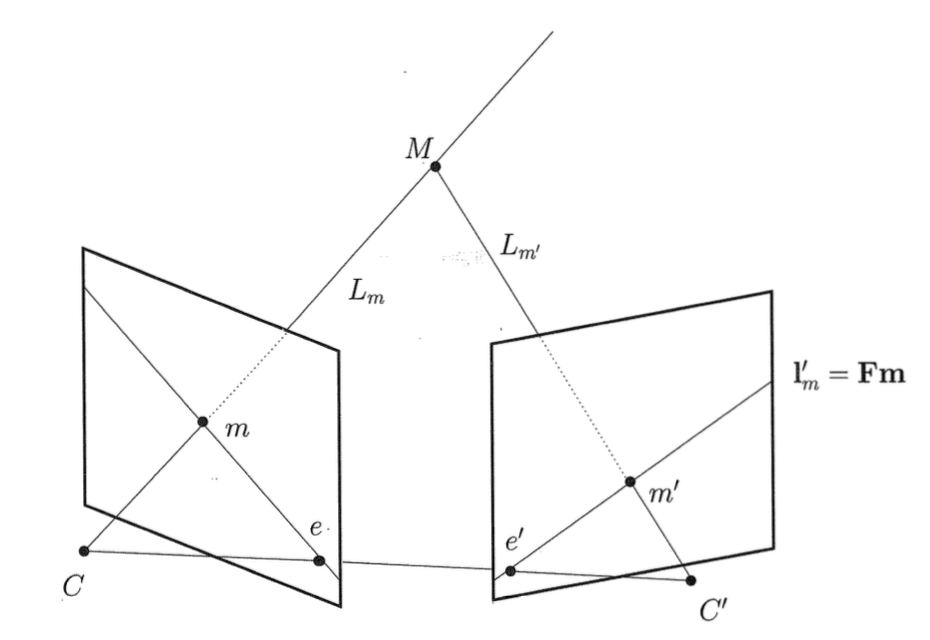
\includegraphics{Imagens/figura2-4.png}
	\caption{Exemplo de geometria epipolar. Dado um ponto $m$, o seu correspondente $m'$ precisa estar na linha epipolar $l'_{m}$. Dada a correspondência válida entre $m$ e $m'$, a interseção dos raios ópticos $Lm$ e $Lm$ é não-vazia, e coplanar com a linha $CC'$. Faugeras et al \cite{Faugeras-Geometry} pag. 25.}
	\label{fig4}
\end{figure}

Normalmente não se assume qualquer relação espacial entre os pontos no espaço, apenas a informação disponível pela correspondência projetiva, ou seja, a correspondência de pontos por projeção linear. A geometria epipolar é a restrição básica que decorre da existência de dois pontos de vista distintos. Ambos podem ser obtidos por duas câmeras diferentes ou com uma câmera em movimento, denominado \textit{Structure from Motion}. As restrições epipolares descrevem totalmente a correspondência de pares de correspondências genéricas entre pontos de cada imagem, e a ambiguidade ao longo da linha epipolar causada pela ambiguidade ao longo dos raios ópticos da operação de projeção. Partindo do fato de que a matriz fundamental depende apenas da geometria da câmera, descreve todas as restrições epipolares, logo compila toda a informação disponível das correspondências projetivas. 

Já que todos os raios ópticos contêm o centro óptico $C$ da primeira câmera, todas as linhas epipolares contêm a projeção de $C$ na segunda imagem nos pontos onde a primeira câmera é vista pela segunda, chamado epipolo. Como mostra a figura \ref{fig2}, o fato do epipolo da segunda imagem pertencer às linhas epipolares significa que $e'^{T}Fm = 0$, ou, $F^{T}e' = 0$. Invertendo as duas imagens, $Fe = 0$. Pode-se concluir que $F$ é uma matriz de grau 3 e $det(F) = 0$. Como essa restrição algébrica é satisfeita e é apenas definida por um fator de escala, $F$ depende de sete parâmetros.

Para o cálculo da matriz fundamental, tem-se $m$ e $m'$ correspondentes abaixo:

\begin{equation}\label{eq5}
m = \begin{bmatrix}u\\v\\1\\ \end{bmatrix}, \; \; \;
m' = \begin{bmatrix}u'\\v'\\1\\ \end{bmatrix}
\end{equation}

Equação \eqref{eq5}: Matrizes dos pontos $m$ e $m'$.

e $F$ a matriz fundamental:

\begin{equation}\label{eq6}
F = 
\begin{bmatrix}
	F_{11} &  F_{12} &  F_{13}\\
	F_{21} &  F_{22} &  F_{23}\\
	F_{31} &  F_{32} &  F_{33}
\end{bmatrix}
\end{equation}

Equação \eqref{eq6}: Matriz fundamental $F$.

Logo, a restrição epipolar $m'^{T}Fm = 0$ pode ser representada como $U^{T}f = 0$, onde:

\begin{equation}\label{eq7}
f = [F_{11}, F_{12}, F_{13}, F_{21}, F_{22}, F_{23}, F_{31}, F_{32}, F_{33}]
\end{equation}
\begin{equation}\label{eq8}
U = [uu', vu', u', uv', vv', v', uv,1]^{T}
\end{equation}

Equações \eqref{eq7}, \eqref{eq8}: Representações de $f$ e $U$.

O sistema de equações $U^{T}f = 0$ é linear, homogêneo e possui 9 incógnitas, com 8 pares de pontos correspondentes. Caso seja possível obter 8 casamentos, então é possível, no geral, obter uma solução única para $F$, definida por um fator de escala. Essa abordagem é conhecida como o algoritmo de 8 pontos.

\section{\textit{Simultaneous Localization And Mapping}}

O termo \textit{SLAM} é a sigla para \textit{Simultaneous Localization And Mapping}. O \textit{SLAM} foi criado a partir do problema de construir um mapa de um ambiente desconhecido por um robô móvel enquanto ao mesmo tempo navega pelo ambiente, podendo utilizar informações parciais do mapa caso estejam disponíveis. O \textit{SFM} consiste em realizar a reconstrução com base em estruturas estáticas, já o \textit{SLAM} tem como objetivo realizar a reconstrução partindo do movimento realizado, seja em tempo real de um \textit{stream} ou um vídeo. O \textit{SLAM} consiste de múltiplas partes: Extração de pontos de referência, associação de dados, estimativa de estados, e atualização de ponto de referência. Há várias formas de resolver cada uma dessas partes menores que pode ser exclusivo de cada implementação\cite{SLAM-Dummies}. Na abordagem padrão para o \textit{SLAM} usa-se sensores a \textit{laser} para estimar a distância entre os pontos de referência e fazer o cálculos com base nesses dados. No caso desse trabalho ao invés de \textit{lasers} e sensores de movimento buscou-se métodos para uso de apenas uma câmera em junção com \textit{Computer Vision e Multiple View Geometry} para que essa implementação possa ser usada potencialmente em dispositivos móveis. O \textit{LSD-SLAM} é uma biblioteca oferece essa abordagem usando gradientes de imagens digitais e por ser o método utilizado, será discutido nas próximas seções.



\section{Algoritmos de detecção de características}
  
Mesmo utilizando câmeras estéreo, ainda existem problemas para mapear estruturas a partir do movimento das câmeras, onde normalmente há duas câmeras sendo utilizadas para obter mais informações sobre um mesmo objeto sob diferentes pontos de vista, mas a correspondência entre as imagens obtidas e os objetos 3D precisam ser encontradas. Para isso, são utilizadas características distintas como cantos, possuindo também diferentes gradientes em múltiplas direções, ou vértices, de uma imagem para outra. O algoritmo mais conhecido atualmente é o \textit{SIFT} \cite{SIFT}, onde utiliza a máxima para a pirâmide de diferença de \textit{Gauss} como características. Primeiramente o \textit{SIFT} procura uma direção dominante no gradiente, e para deixá-lo invariante à rotação, rotaciona o descritor para que sua orientação seja compatível.
  
  As características adquiridas ao longo do tempo são usadas para reconstruir suas localizações no espaço 3D e o movimento da câmera. Outra alternativa são as “abordagens diretas”, que tentam obter as informações geométricas sem abstração intermediária como características ou cantos.

O \textit{SURF}\cite{SURF} também é um algoritmo conhecido na tarefa de obter características, mas ao invés de obter as diferenças de \textit{Gauss}, se baseia em determinantes de matrizes Hessianas para localização e escala \cite{Hessian}. E ao invés de calcular histogramas dos gradientes, computa a soma dos componentes destes com seus valores absolutos. Todas as características detectadas de todas as imagens então são combinadas.

O \textit{ORB (Oriented FAST and Rotated BRIEF)} surgiu como uma alternativa ao algoritmo de detecção e descrição de pontos característicos \textit{SIFT} na questão de eficiência em smartphones, já que se mostra mais eficiente em dispositivos com menos poder de processamento, bem como não ser patenteado, ao contrário do \textit{SIFT} e \textit{SURF}, podendo acarretar em problemas de propriedade intelectual. O \textit{ORB} toma como base a detecção de pontos característicos do \textit{SIFT} e o descritor do \textit{BRIEF}, já que ambos são bem eficientes nestas tarefas e baixo custo computacional. Um dos problemas demonstrados por \textit{Rublee et al}\cite{ORB-Artigo} em seu artigo é a falta de invariância com relação à rotação no \textit{BRIEF}.

Como dito anteriormente, o algoritmo \textit{FAST} foi escolhido para detecção de \textit{keypoints} em sistemas em tempo real que procuram um casamento isto é, encontrar a similaridade entre duas imagens, entre características visuais, mas o algoritmo precisava ser incrementado com a pirâmide de \textit{schemes} para escala\cite{ORB-Artigo} e o filtro de Harris\cite{ORB-Artigo} para rejeitar cantos. Ao contrário do \textit{SIFT} e \textit{SURF}, o \textit{FAST} não provém de um operador de orientação. Como descrito em seu artigo, há várias formas de se descrever a orientação de um \textit{keypoint}. Algumas destas formas envolvem computações de histogramas de gradientes, mas tais métodos são muito ostensivos computacionalmente e no caso do \textit{SURF}, levando à aproximações não muito boas.

Para os descritores, o \textit{BRIEF} é utilizado pela robustez para luz, \textit{blur} e distorção de perspectiva, mas é sensível com a rotação do plano \cite{ORB-Artigo}. O \textit{BRIEF} utiliza testes binários para treinar um conjunto de árvores de classificação \cite{ORB-Artigo}, normalmente treinadas com 500 ou mais \textit{keypoints}, podem ser utilizadas para retornar a assinatura de um \textit{keypoint arbitrário} \cite{ORB-Artigo}.

Infelizmente as combinações encontradas podem ser errôneas, logo é preciso eliminar falsos positivos. Para isso normalmente se é utilizado o \textit{RANSAC}, algoritmo que remove combinações de pontos \textit{outliers}, isto é, combinações que provavelmente não pertencem ao espaço. O \textit{RANSAC} também é utilizado para resolver o \textit{Location Determination Problem}, que tem como objetivo determinar os pontos no espaço que têm projeção numa imagem com localizações conhecidas \cite{RANSAC}.

As características adquiridas ao longo do tempo são usadas para reconstruir suas localizações no espaço 3D e o movimento da câmera. Outra alternativa são as “abordagens diretas”, que tentam obter as informações geométricas sem abstração intermediária como características ou cantos.
  
\section{Bibliotecas}
  
\subsection{\textit{FIT3D}}
O \textit{FIT3D} foi desenvolvido por Esteban et al\cite{FIT3D}, com o intuito de ser uma ferramenta única para realizar os 5 passos do processo de reconstrução de uma cena, que são: calibração da câmera, estimação de movimento, otimização, reconstrução e modelagem. Foi criado para \textit{MATLAB}® e é composto de várias funções próprias bem como de pacotes de terceiros como o \textit{SIFT}, utilizadas em seu \textit{pipeline} para reconstruir a cena, composto pelas seguintes fases:
\begin{description}
 \item[Calibração: ]{Processo de obter os parâmetros intrínsecos que descrevem a câmera. Inclui parâmetros para distorção radial, como mostrado no livro de Faugeras cap 4.5 e 4.6 \cite{Faugeras-Geometry}, distância focal, centro de projeção e parâmetros \textit{skew};}
 \item[Egomotion (odometria visual): ]{É a estimativa de movimento de uma câmera entre quadros baseada na informação obtida das imagens denominada como parâmetros extrínsecos. No \textit{FIT3D}, apenas quadros consecutivos são considerados para movimento;}
 \item[Refinamento: ]{Dado que as imagens são obtidas com ruído e este é propagado para a estimação de movimento, é desejável que haja uma otimização para melhorar as estimativas;}
 \item[Reconstrução: ]{Partindo das posições das câmeras, parâmetros de calibração e as imagens, a reconstrução é o processo de se obter uma representação 3D da cena bem como um conjunto de pontos 3D;}
 \item[Modelagem: ]{Processo de converter uma nuvem esparsa de pontos 3D em algo de maior ordem, como um plano, superfície ou modelo.}
\end{description}
  
 Para obter a distorção radial, o \textit{FIT3D} utiliza o método de \textit{Zhang} \cite{FIT3D}. Infelizmente, o \textit{FIT3D} não é atualizado desde 2010, acarretando numa documentação e código obsoletos, e diversos bugs foram encontrados durantes os testes realizados, inclusive impedindo o processamento da reconstrução do nosso \textit{dataset}. Outro problema encontrado é a falta de uma forma que seja possível executar o algoritmo ao vivo, ao contrário do \textit{LSD-SLAM} apresentado na próxima seção.

\subsection{\textit{LSD-SLAM}}

Um dos maiores benefícios do \textit{SLAM} monocular, e simultaneamente o seu maior desafio, vem da sua ambiguidade de escala inerente: A escala do mundo não pode ser observada e muda com o tempo, sendo uma das maiores fontes de erro. A vantagem é que isso permite a troca entre ambientes de diferentes escalas, como ambientes internos com móveis e ambientes externos. Por outro lado sensores escalonados como câmeras estéreo e câmeras de profundidade fornecem resultados mais confiáveis mas não oferecem a mesma flexibilidade tanto na facilidade de troca entre diferentes escalas quanto no \textit{hardware}, fazendo a abordagem monocular funcionar para câmeras de celular que é um \textit{hardware} mais acessível. 

\subsubsection{Transformadas de corpo rígido 3D}

Uma transformada de corpo rígido: $\mathbf{G} \in se(3)$ denota rotação e translação em 3D e é definida pela equação \eqref{eq3d}: 

\begin{equation}\label{eq3d}
	\mathbf{G} = \begin{pmatrix}
	\mathbf{R} & \mathbf{t} \\
	0 & 1\end{pmatrix}
\quad sendo \quad \mathbf{R} \in SO(3) \quad e \quad \mathbf{t} \in \mathbb{R}^3.
\end{equation}

Equação \eqref{eq3d}: Transformada de corpo rígido 3D

A representação mínima de pose de câmera é dada pelo elemento correspondente $\mathbf{\xi} \in se(3)$ \cite[p. 4]{LSD-SLAM-Artigo}.

\subsubsection{Transformada de similaridade 3D}

Uma transformada de similaridade 3D: $\mathbf{S}\in sim(3)$ denota rotação, escala e translação e é definida pela equação \eqref{eq3d2}:
 
 \begin{equation}\label{eq3d2}
 \mathbf{S} = 
 \begin{pmatrix}
 \mathbf{R} & \mathbf{t} \\
 0  & 1
 \end{pmatrix}
\quad com \quad \mathbf{R} \in SO(3), \quad \mathbf{t} \in \mathbb{R}^{3} \quad e \quad s \in \mathbb{R}^+.
 \end{equation} 

Equação \eqref{eq3d2}: Transformada de similaridade 3D
 
A representação mínima da transformada de similaridade é dada pelo elemento correspondente $\mathbf{\xi} \in sim(3)$ \cite[p. 5]{LSD-SLAM-Artigo}.

\subsubsection{Componentes do \textit{LSD-SLAM}}

Segundo o artigo do \textit{LSD-SLAM} \cite{LSD-SLAM-Artigo}, o algoritmo consiste de três componentes principais: \textbf{\textit{tracking}} (rastreamento), \textbf{\textit{depth map estimation}} (estimativa de mapa de profundidade) e \textbf{\textit{map optimization}} (otimização de mapa):

\begin{itemize}
	\item{O componente de \textbf{\textit{tracking}} continuamente rastreia novas imagens de câmera; Isso é, ele estima sua pose de corpo rígido, dado por $\mathbf{\xi} \in se(3)$, com relação ao quadro-chave atual, usando a pose do quadro anterior como inicialização.}
	\item{O componente de \textbf{\textit{depth map estimation}} usa quadros rastreados para refinar ou repor o quadro-chave atual. A profundidade é refinada filtrando, entre várias comparações estéreo de pequeno patamar por \textit{pixel}, casadas com regularização espacial intervalada. Se a câmera se mover muito longe, um novo quadro-chave é inicializado projetando os pontos de quadros-chave perto já rastreados nele.}
	\item{Assim que o componente do \textbf{\textit{depth map estimation}} define que a imagem atual não deve ser usada para refinamento, mas como um novo quadro-chave, o anterior é reposto pela nova imagem que se torna um quadro-chave. O mapa de profundidade do quadro chave anterior não será mais refinado e é incorporado ao mapa global pelo componente de \textbf{\textit{map optimization}}. Para detectar fechamentos de \textit{loops} e mudança de escala, uma transformada de similaridade, dada por $\mathbf{\xi} \in sim(3)$, é estimada para \textit{keyframes} próximos já capturados.}
\end{itemize}	
\chapter{Metodologia}

A metodologia deste trabalho foi dividida em duas partes: A obtenção dos dados da câmera, bem como \textit{keypoints} e \textit{keyframes} partindo da câmera de um \textit{smartphone} utilizando um aplicativo de autoria própria, o \textit{PhotoGuide}; e a reconstrução do ambiente utilizando a ferramenta \textit{LSD-SLAM}. O \textit{PhotoGuide} não foi usado na segunda parte do projeto devido à baixa performance e do baixo suporte nativo da ferramenta \textit{OpenCV} para \textit{Android} fazendo a reconstrução 3D ser migrada do \textit{smartphone} para uma ferramenta \textit{desktop}.


\section{\textit{PhotoGuide}}

Desenvolvido para a plataforma \textit{Android}®, o \textit{PhotoGuide} \cite{PhotoGuide} teve como objetivo primário a reconstrução de ambientes à partir da câmera do dispositivo que fosse executado da plataforma \textit{Android}. O aplicativo utiliza diversos algoritmos providos pela biblioteca de terceiros \textit{OpenCV} \cite{OpenCV}. O objetivo do \textit{PhotoGuide} é, partindo do \textit{stream} da câmera ou recebendo um conjunto de imagens sequenciais, obter os quadros num intervalo pré-determinado e então enviar pares para serem processados utilizando o \textit{ORB}, retornando os \textit{keypoints} encontrados depois de filtrados, sendo inseridos num banco de dados no final do processo.  Primeiramente foi necessário obter os \textit{keypoints} da cena, e os algoritmos mais utilizados para isso são \textit{SIFT} e \textit{SURF}, mas infelizmente ambos são patenteados, o que nos obrigaria a lidar com a questão das patentes e permissão de uso. O \textit{ORB} e \textit{BRISK} são algoritmos para obter \textit{keypoints} e seus descritores, e foram desenvolvidos para terem um desempenho semelhante ao \textit{SIFT} e\textit{ SURF}, tornando-se assim a melhor escolha já que são de livre uso.

Primeiramente, os \textit{keypoints} são obtidos diretamente da câmera do aparelho, mas a taxa de captura usada foi 10\textit{FPS}, e passados (como imagens \textit{bitmap} e em pares) para o \textit{ORB}; então são processado os \textit{keypoints} e seus descritores, mas infelizmente é possível haver ruído na imagem e, portanto, ocasionando em falsos casamento entre uma imagem e outra. Para remover o máximo possível de falsos positivos, foram utilizadas três técnicas de refinamento, na ordem: \textit{Cross Check}, \textit{Ratio Filtering} e \textit{RANSAC}.

Ao executar o \textit{ORB} e \textit{BRISK}, são obtidas estruturas que possuem informações acerca do \textit{keypoint}, bem como informações sobre seu correspondente na segunda imagem. O \textit{Cross Check} consiste em rodar o algoritmo duas vezes, uma procurando pontos da primeira imagem na segunda, e outra vez procurando pontos da segunda imagem na primeira. Por fim, percorre ambos, verificando se para cada casamento da primeira lista, as informações batem com o casamento correspondente da segunda lista.

O \textit{Ratio Filtering} percorre a lista resultante, verificando se há mais de um casamento para cada \textit{keypoint}, já que o ideal é que cada \textit{keypoint} tenha apenas um único correspondente na segunda imagem. Ao encontrar mais de uma ocorrência, descarta os pontos mais distantes.

Por fim, a última filtragem é realizada com o \textit{RANSAC} \cite{RANSAC}. O \textit{RANSAC} é um método iterativo para estimar parâmetros de modelos matemáticos partindo de um conjunto de informações obtidas que possuem \textit{outliers}. Também é considerado um método determinístico que possui um bom resultado com confiabilidade. Foi apresentado em 1981 por Fischler e Bolles para tentar resolver o problema da determinação da localização. Ele parte do princípio que o conjunto de informações possui \textit{inliners}, os quais são informações que podem ser explicadas pelos parâmetros do modelo, apesar que podem ter sofrido ruído, e os \textit{outliers}, que são informações que não condizem com o modelo. Esses \textit{outliers} podem ser provenientes de ruído, medições errôneas ou uma má interpretação das informações. A figura \ref{fig3:1} possui um exemplo de um conjunto de informações, os pontos, e como o \textit{RANSAC} trataria os \textit{inliners} e \textit{outliners}:

\begin{figure}
	\centering
		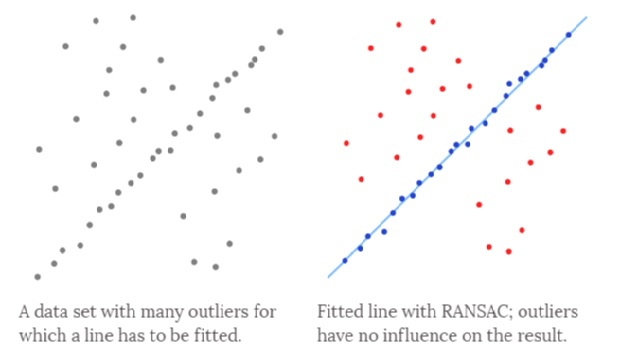
\includegraphics{Imagens/figura3-1.jpg}
	\caption{Exemplificação do tratamento do \textit{RANSAC} com os \textit{inliners} e \textit{outliners}. Imagem licenciada pela CC 3.0}
	\label{fig3:1}
\end{figure}
  

Por fim, as comparações entre as imagens eram retornadas, e seus \textit{keypoints} armazenados num banco de dados, para futuro processamento. A figura \ref{fig3:2} mostra um exemplo da execução do aplicativo:

\begin{figure}[H]
	\centering
		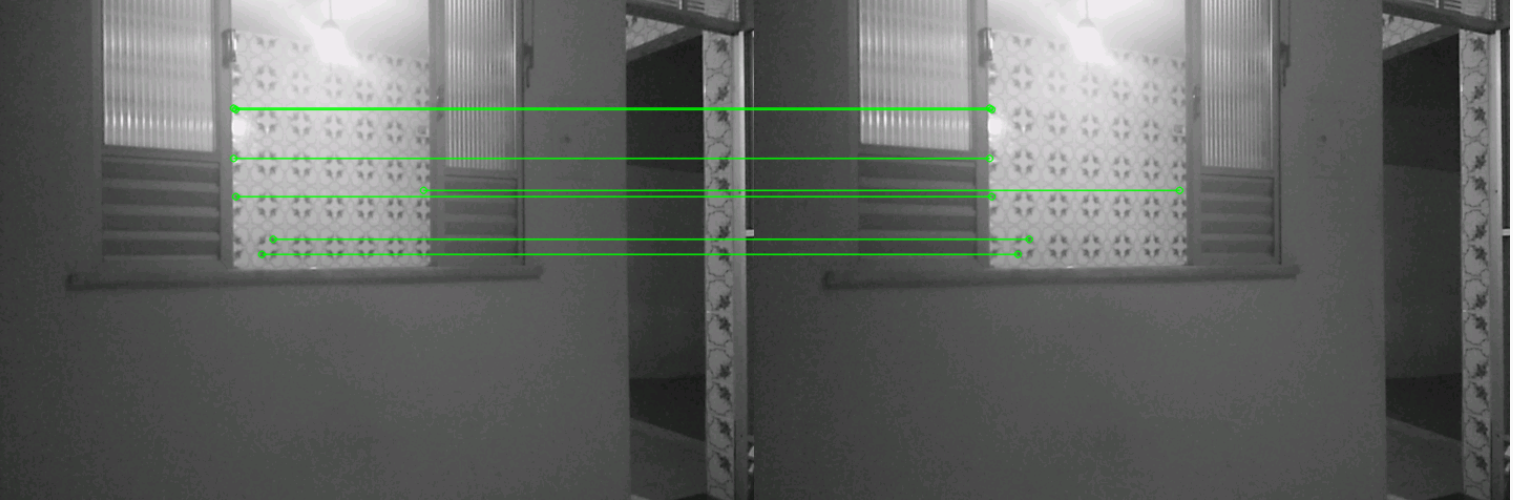
\includegraphics[width= \textwidth]{Imagens/figura3-2E4-4.png}
	\caption{\textit{Keypoints} encontrados e filtrados entre duas imagens.}
	\label{fig3:2}
\end{figure}

 
Foi adicionado ao aplicativo a opção de realizar a calibração da câmera com o auxílio da biblioteca \textit{OpenCV}, já que foi percebido que a distorção radial da câmera estava influenciando os resultados. A calibração da câmera, numa forma prática, consiste em fornecer um \textit{stream} da câmera ou sequência de fotos, contendo um padrão pré-definido. O \textit{OpenCV} fornece funções para calibrar a câmera de um dispositivo, necessitando das imagens capturadas do padrão, dentre as seguintes opções:

\begin{itemize}
	\item{Tabuleiro de xadrez em \ref{fig3:3}}
	\item{Círculos alinhados assimetricamente em \ref{fig3:4}}
	\item{Círculos alinhados simetricamente em \ref{fig3:5}}
\end{itemize}

\begin{figure}[H]
\minipage{0.32\textwidth}
  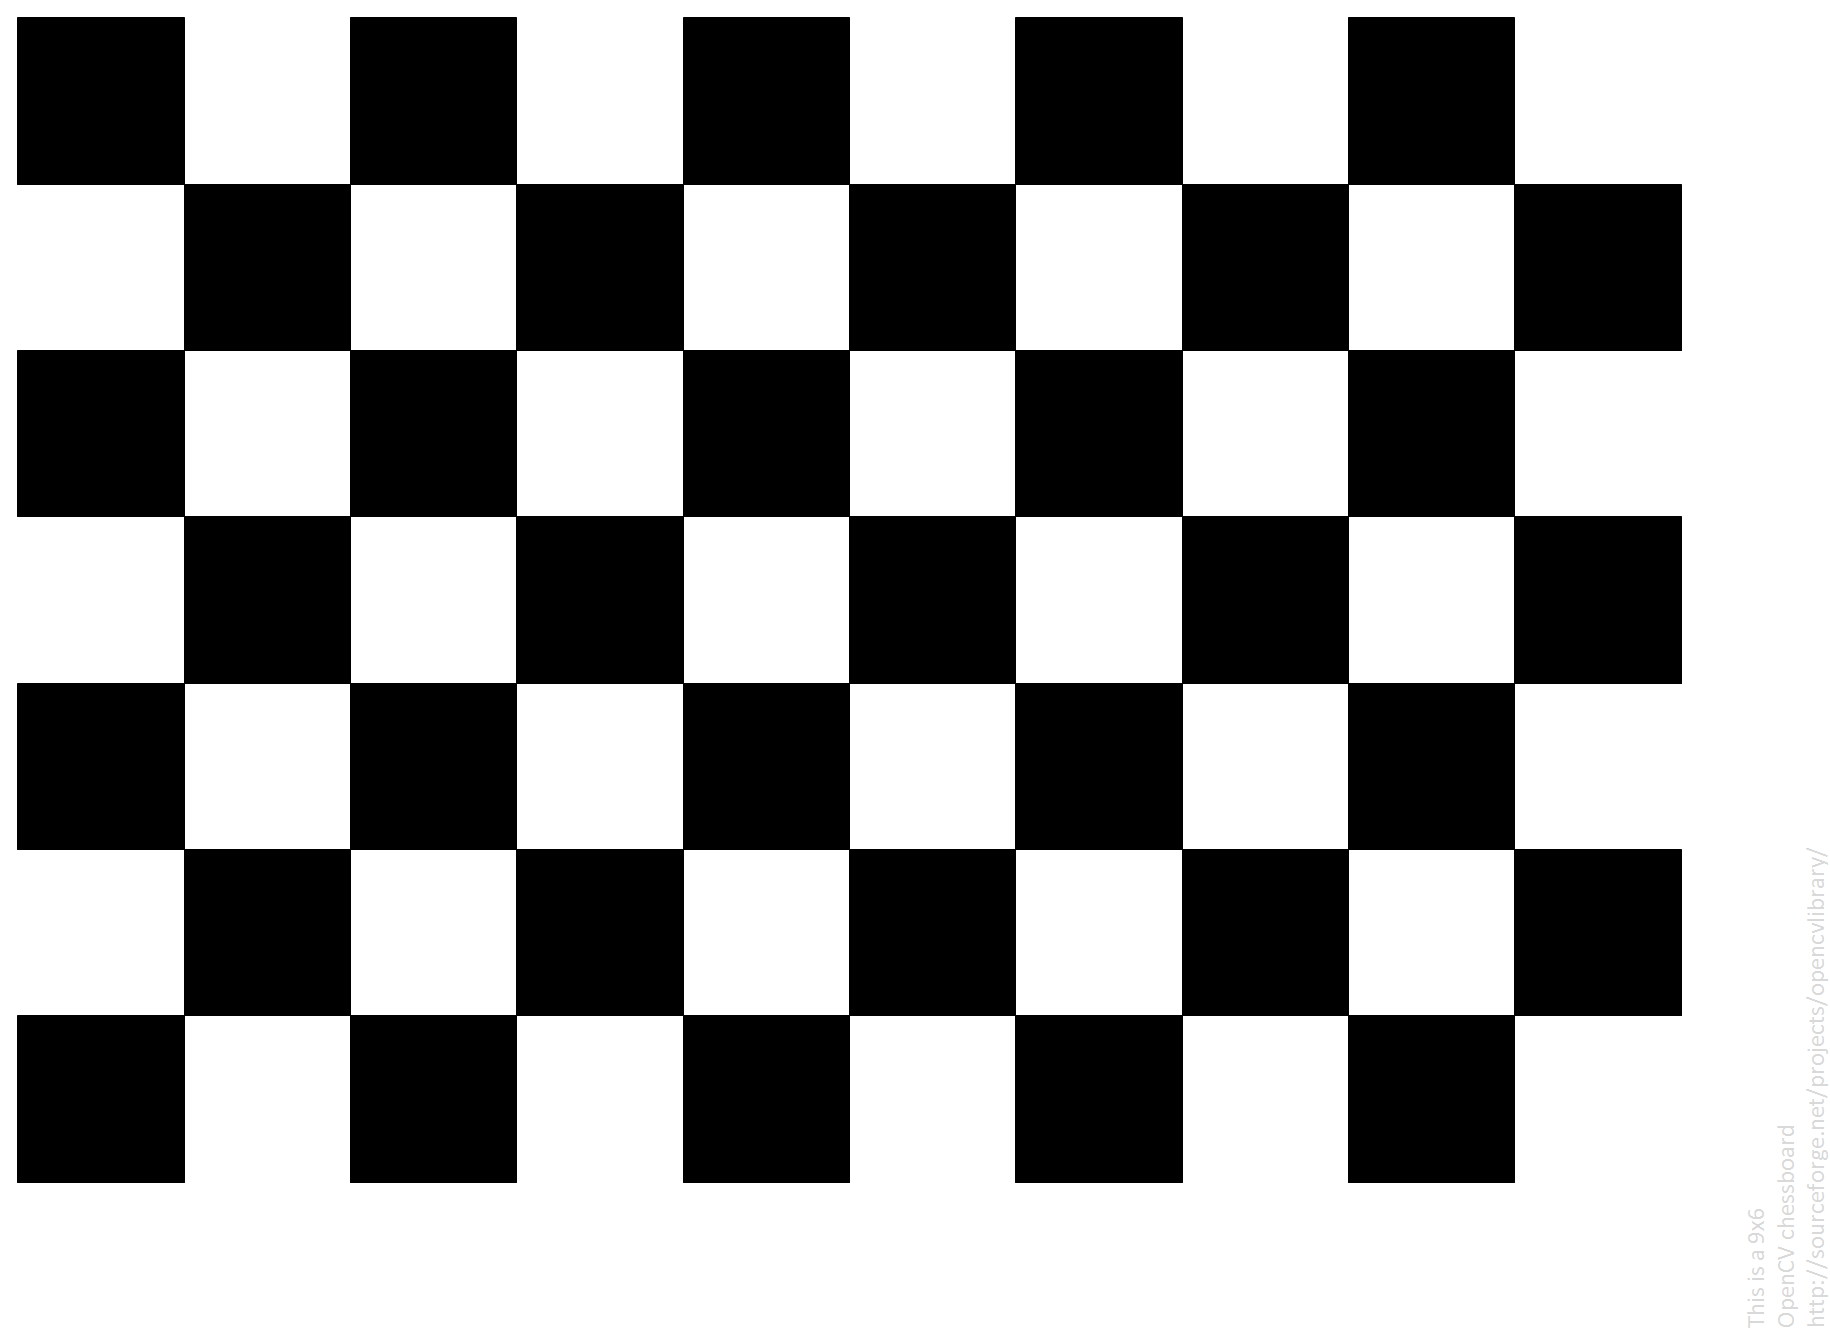
\includegraphics[width=\linewidth]{Imagens/figura3-3E3-12.png}
  \caption{Tabuleiro de xadrez}\label{fig3:3}
\endminipage\hfill
\minipage{0.32\textwidth}
  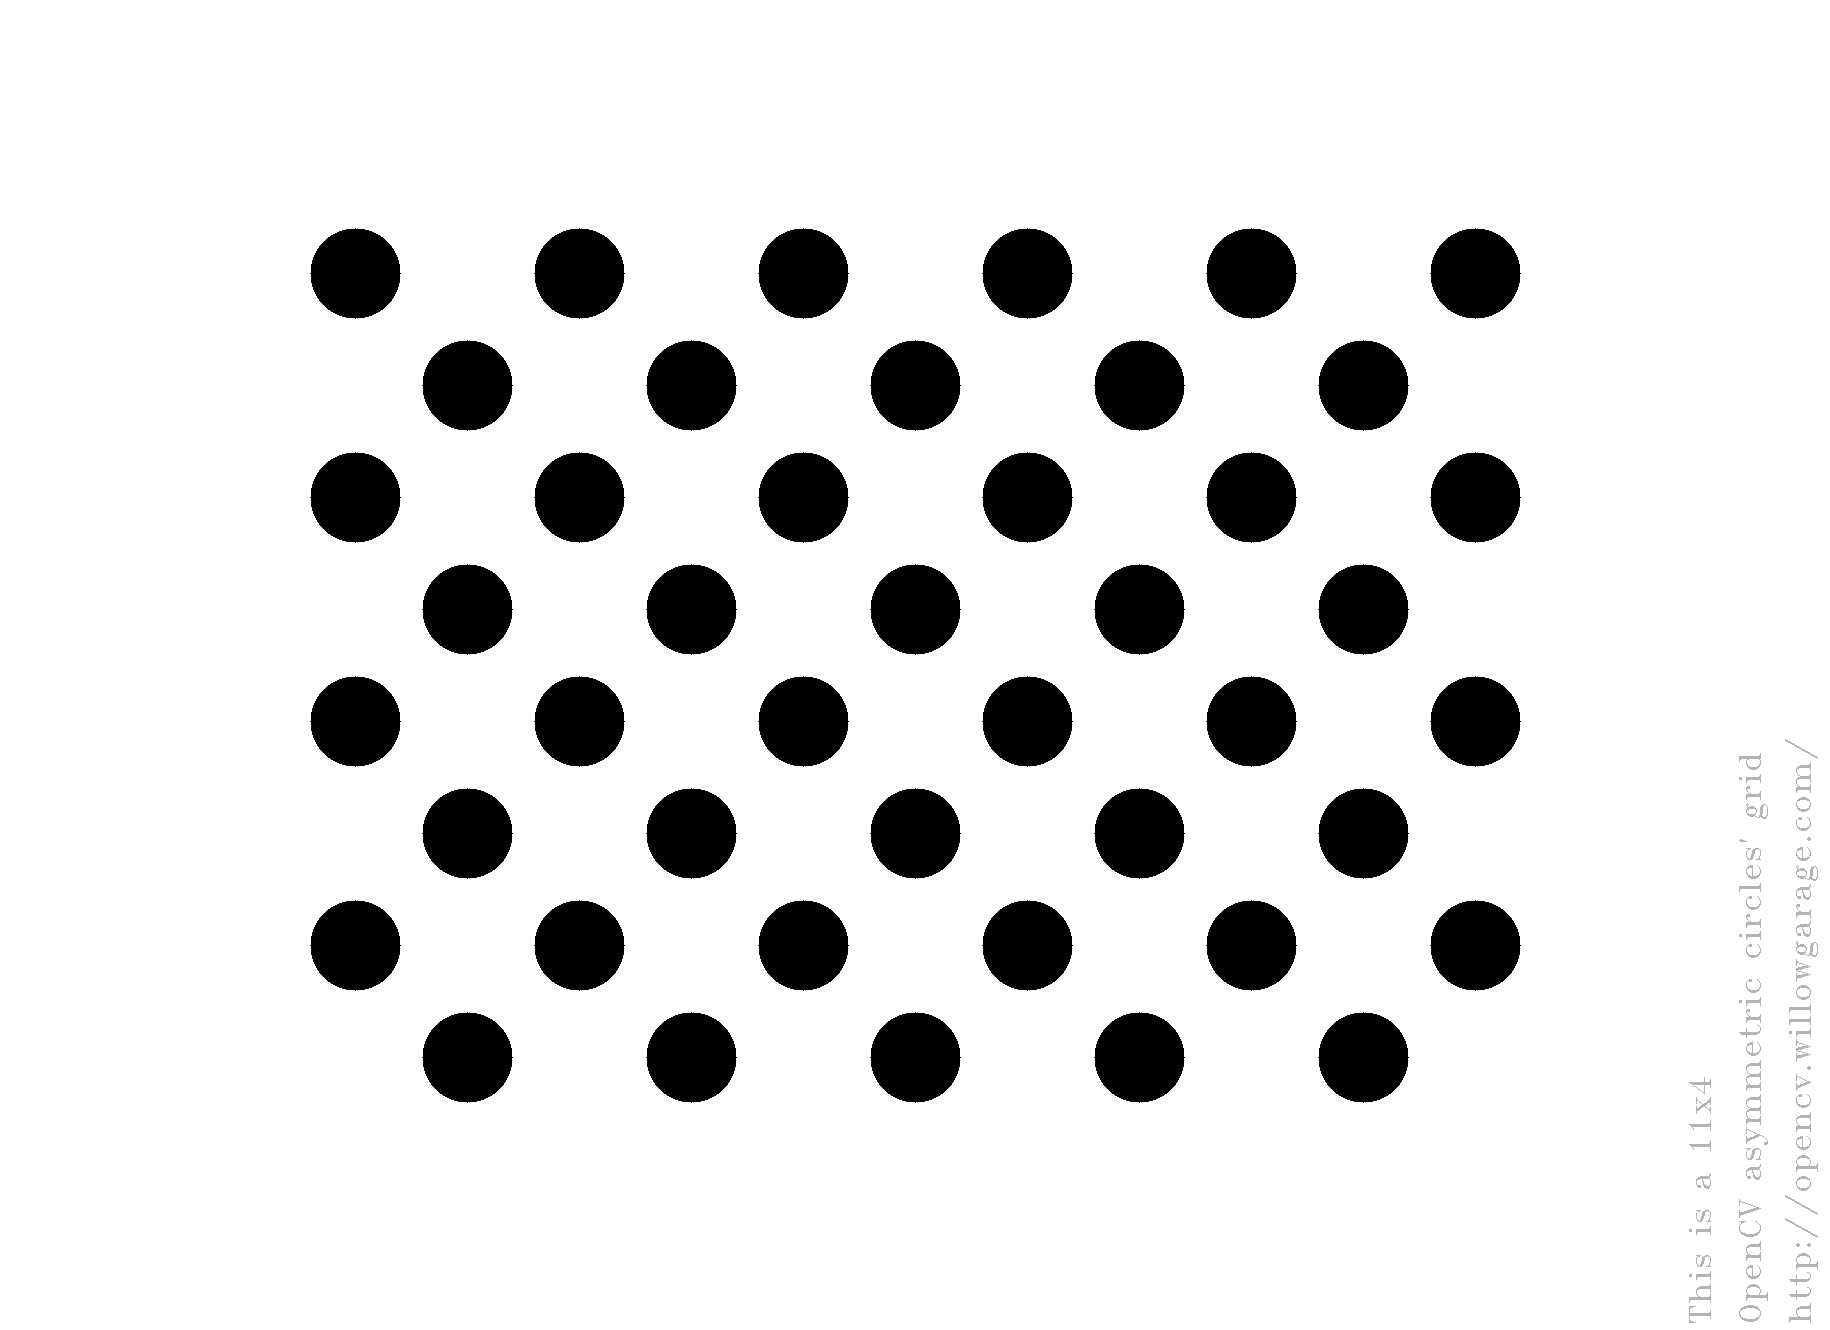
\includegraphics[width=\linewidth]{Imagens/figura3-4.png}
  \caption{Círculos alinhados assimetricamente}\label{fig3:4}
\endminipage\hfill
\minipage{0.32\textwidth}
  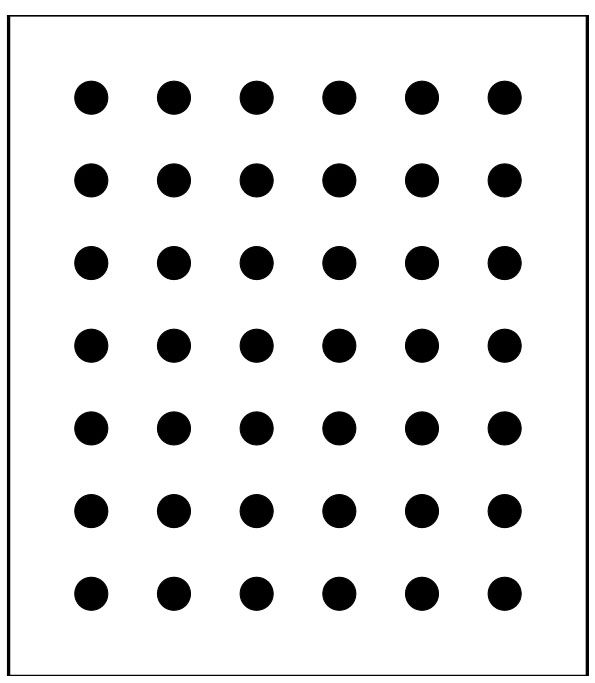
\includegraphics[width=\linewidth]{Imagens/figura3-5.jpg}
  \caption{Círculos alinhados simetricamente}\label{fig3:5}
\endminipage
\end{figure}


\begin{figure}[!hb]
\minipage{0.49\textwidth}
  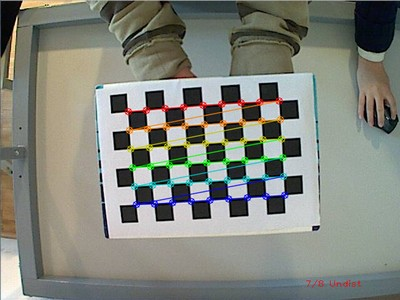
\includegraphics[width=\linewidth]{Imagens/figura3-6.jpg}
  \caption{Reconhecimento do tabuleiro de xadrez}\label{fig3:6}
\endminipage\hfill
\minipage{0.49\textwidth}
  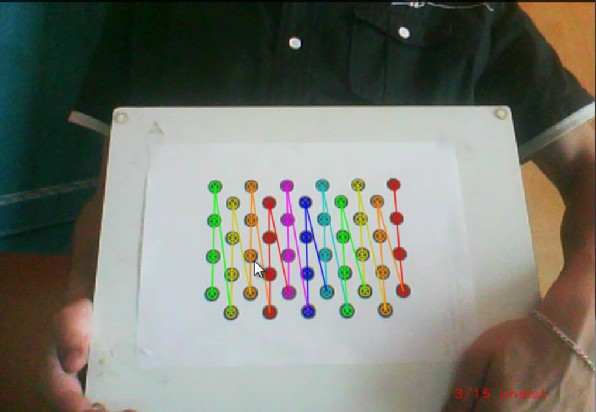
\includegraphics[width=\linewidth]{Imagens/figura3-7.jpg}
  \caption{Reconhecimento dos círculos alinhados assimetricamente}\label{fig3:7}
\endminipage
\end{figure}

Ao fim da calibração, o algoritmo retorna a matriz de calibração da câmera, que servirá para remover a distorção radial das imagens capturadas posteriormente; vale frisar que a distorção radial será removida somente se  a matriz de calibração tenha sido calculada corretamente. As figuras \ref{fig3:8},\ref{fig3:9},\ref{fig3:10} e\ref{fig3:11} mostram mais exemplos da execução do aplicativo para obter \textit{keypoints} bem como imagens da mesma cena sem filtragem de \textit{keypoints}

\begin{figure}[H]
	\centering
		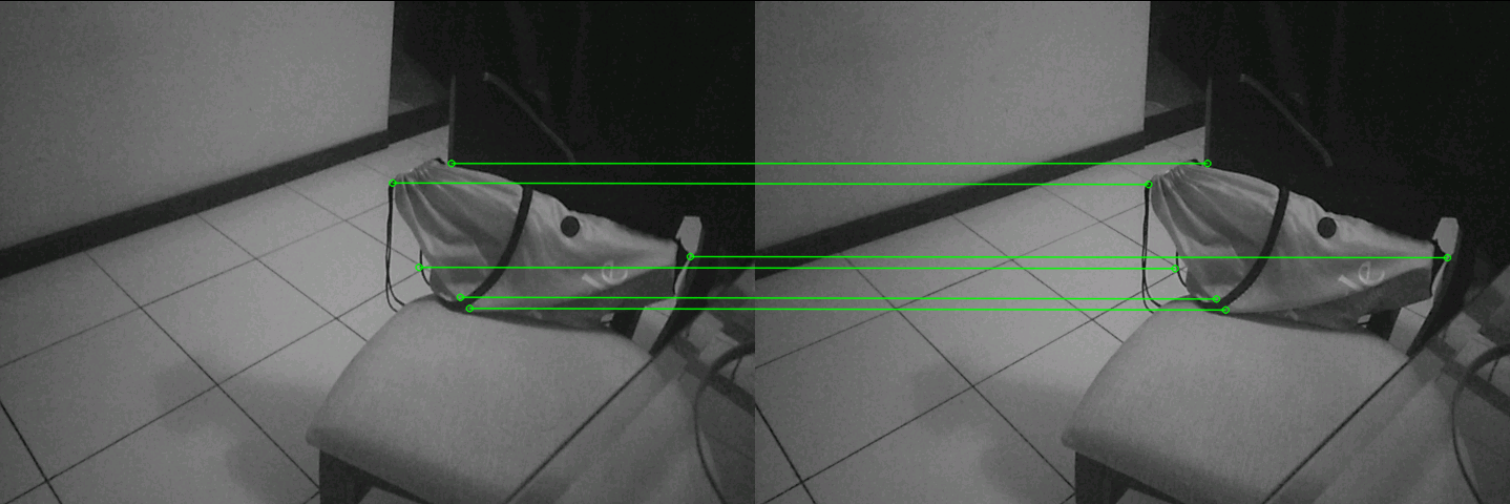
\includegraphics[width= \textwidth]{Imagens/figura3-8.png}
	\caption{Execução do \textit{PhotoGuide} e os \textit{keypoints} filtrados da cena \#1}
	\label{fig3:8}
\end{figure}

\begin{figure}[H]
	\centering
		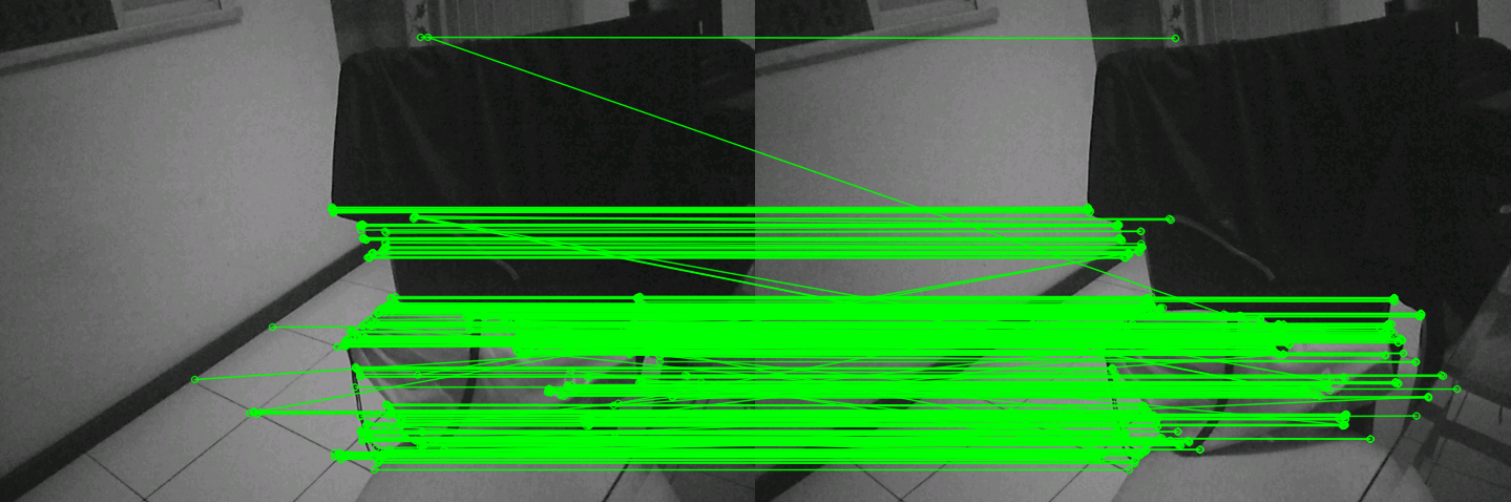
\includegraphics[width= \textwidth]{Imagens/figura3-10.png}
	\caption{\textit{Keypoints} não filtrados da cena \#1}
	\label{fig3:9}
\end{figure}

\begin{figure}[H]
	\centering
		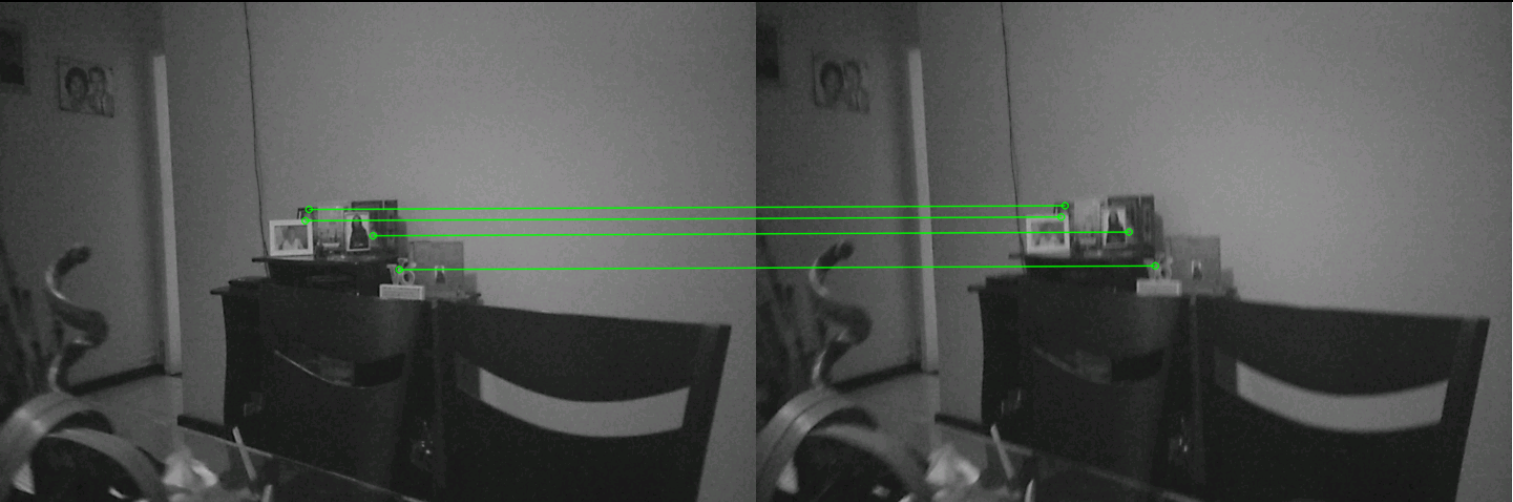
\includegraphics[width= \textwidth]{Imagens/figura3-9.png}
	\caption{Execução do \textit{PhotoGuide} e os \textit{keypoints} filtrados da cena \#2}
	\label{fig3:10}
\end{figure}

\begin{figure}[H]
	\centering
		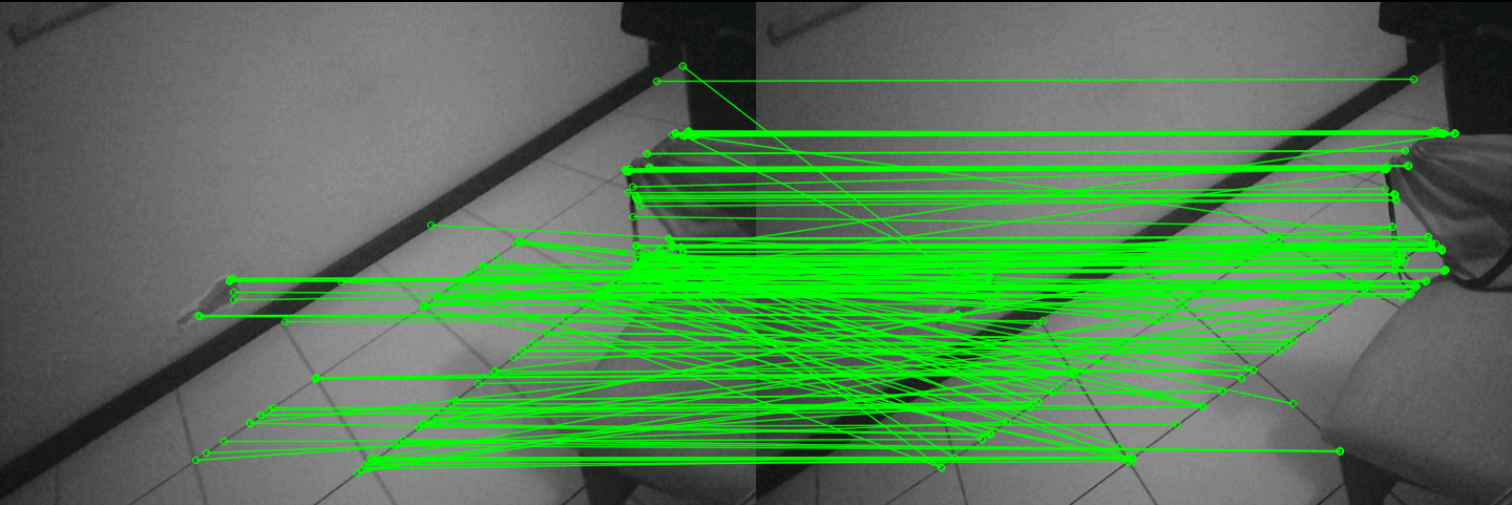
\includegraphics[width= \textwidth]{Imagens/figura3-11.png}
	\caption{\textit{Keypoints} não filtrados da cena \#2}
	\label{fig3:11}
\end{figure}


É possível perceber a importância de se detectar e remover falsos positivos, ou \textit{outliers}, já que essa quantidade de pontos errôneos afetaria drasticamente o processamento.

\subsection{Dificuldades Encontradas}

Durante o desenvolvimento do \textit{PhotoGuide}, certos problemas causaram grande dificuldade para a continuação de sua implementação. A ausência de documentação, bem como o tamanho pequeno da comunidade de desenvolvimento utilizando \textit{OpenCV} no \textit{Android} dificultam a pesquisa por casos semelhantes ou para a procura de auxílio com o código fonte, bem como a questão de que a maior parte dos resultados encontrados são escritos para a linguagem \textit{C++}, que é mais permissiva do que \textit{Java}®, a linguagem utilizada no desenvolvimento do \textit{PhotoGuide}. Outros problemas provenientes disso são as diferenças entre implementações, já que em \textit{C++}, é possível realizar diversas operações entre os tipos de \textit{Mat},  que é uma estrutura do \textit{OpenCV} para armazenar informações acerca de uma matriz, fato que não é possível em \textit{Java} já que os diferentes objetos \textit{Mat} na versão do \textit{OpenCV} para \textit{Java} são de classes diferentes e não possuem comportamento semelhante. Para certas tarefas, era possível utilizar o \textit{JNI (Java Native Interface)}\cite{JNI}, que permite que código escrito em \textit{Java }realize chamadas para códigos escritos em linguagens compiladas, como por exemplo C e C++, e neste deste trabalho, foi testado algumas implementações do \textit{OpenCV} em \textit{C++}. O \textit{JNI} é utilizado principalmente quando se é necessário utilizar uma biblioteca já implementada em outra linguagem que seja compilada, ou quando a complexidade do código na outra linguagem possui uma menor complexidade. No \textit{PhotoGuide}, não foram encontradas melhorias significativas utilizando \textit{JNI}. 

Outro problema encontrado foi o baixo desempenho, já que a captura constante de quadros junto ao processamento de pares se mostrou demasiadamente onerosa para serem executados num \textit{smartphone}. Tendo em vista esses problemas, optamos  apenas que a captura de quadros e vídeo fosse feita utilizando a \textit{PSEye}® e depois de um tempo usando vídeo capturado de \textit{smartphone} e extraído os seus quadros usado um \textit{software} a parte, e o processamento fosse feito numa máquina de maior poder de processamento, como um \textit{desktop} ou \textit{laptop}.

\section{\textit{LSD-SLAM}}

A abordagem seguinte adotada no projeto foi a reconstrução de ambientes utilizando o \textit{LSD-SLAM}. O \textit{LSD-SLAM} é uma ferramenta poderosa porém com pouca documentação, o uso dela se mostra trabalhoso devido ao número grande de parâmetros de configuração possíveis e condições de luz e posição, cada ambiente possui suas próprias configurações otimizadas. A capacidade dessa ferramenta de exportar seus mapas 3D em um tipo de arquivo de fácil leitura faz dela facilmente adaptável para qualquer projeto de navegação 3D e reconhecimento espacial. Aprimoramentos em usabilidade e documentação são desejáveis para futuras versões dessa ferramenta caso seus desenvolvedores continuem a atualizando. Nessa seção serão discutidos particularidades de configuração, uso, funcionamento e métodos da utilização dessa ferramenta.

\subsection{Configurações utilizadas}

O \textit{LSD-SLAM} foi testado nas seguintes configurações de máquina, um \textit{desktop} e um \textit{laptop}, respectivamente:

\begin{itemize}
	\item{Processador	\textit{AMD FX™-8350 Eight-Core Processor}, 4000 Mhz, 4 Núcleos, 8 Processadores Lógicos}
	\item{8GB de memória \textit{RAM}}
	\item{Placa gráfica \textit{AMD Radeon R2 260x}}
\end{itemize}

e:

\begin{itemize}
	\item{Processador \textit{Intel® Core™ i3 M370}, 2399 Mhz, 2 Núcleos, 4 Processadores Lógicos}
	\item{4GB de memória \textit{RAM}}
	\item{Placa gráfica integrada: \textit{Intel® HD Graphics}}
\end{itemize}	

Softwares e periféricos utilizados:

\begin{itemize}
	\item{\textit{Ubuntu} versão 14.04\cite{Ubuntu}}
	\item{Câmera \textit{PSEye®}, modelo para o \textit{console} \textit{PlayStation®} 3.}
	\item{Câmera embutida no \textit{smartphone Motorola® Moto X Play} 32GB em junção com o aplicativo \textit{OpenCamera} para \textit{Android}.}
	\item{\textit{Software VLC} para extrair os quadros dos vídeos capturados pela câmera.}
	\item{\textit{Software ROS Indigo}.\cite{ROS-Tutorial}}
	\item{\textit{Driver} para \textit{webcam} \texttt{usb\_cam}.\cite{Setup-USBCAM}}
\end{itemize}

No começo da utilização do \textit{LSD-SLAM} foi testada a câmera \textit{Logitech® HD Webcam c270}, porém essa câmera não oferecia a capacidade mínima recomendado pelo \textit{LSD-SLAM} para obter resultados decentes, que era ter taxa de quadros de pelo menos 30 \textit{FPS} e \textit{global shutter}, em que todos os \textit{pixels} do quadro são expostos ao mesmo tempo, a \textit{PSEye®} se enquadrava em ambos os requisitos e foi usada no lugar da \textit{Logitech}. No entanto usar a câmera \textit{PSEye®} apesar de permitir um resultado melhor, era uma câmera \textit{USB} que devido a mobilidade da câmera estava limitada ao cabo além do próprio tamanho e peso do \textit{notebook} limitava a captura de \textit{datasets} a ser feita usando um \textit{notebook} com a \textit{PSEye®} conectada. Após algum tempo usando a \textit{PSEye®}, os testes foram migrados para a câmera do \textit{smartphone Motorola® Moto X Play}, que tem como diferencial a sua captura de vídeos em mais de 30\textit{FPS} em alta taxa de \textit{bits}. Apesar da câmera não ser \textit{global shutter} e sim \textit{rolling shutter}, em que os \textit{pixels} são expostos sequencialmente em uma direção, que é mais comum entre câmeras \textit{smartphone}, o resultado for satisfatório para o objetivo do trabalho de oferecer o mapeamento 3D do ambiente a partir de um aparelho móvel. A calibração da câmera \textit{smartphone} foi obtida a partir da calibração do \textit{PhotoGuide} e usada como parâmetro para o \textit{LSD-SLAM} usando o método de conversão na seção 3.2.3.7.

\subsection{Captura dos \textit{datasets}}

Os \textit{datasets} capturados foram os seguintes:

\begin{itemize}
	\item{Fachada do DCOMP virada para o estacionamento usando a câmera \textit{PSEye®} - 6180 imagens - 119621 pontos}
	\item{Jardim de área residencial usando a câmera \textit{PSEye®} - 660 imagens - 87093 pontos}
	\item{Sala de Mestrado II usando a câmera \textit{PSEye®} - número de imagens desconhecido por ter sido feito usando o \texttt{live\_slam} sem salvar as imagens - 168915 pontos}
	\item{Fachada do DCOMP virada para o estacionamento usando a câmera do \textit{smartphone Motorola® Moto X Play} 32GB- 3280 imagens - 3680087 pontos}
	\item{Corredor interno do 1º andar do DCOMP usando a câmera do \textit{smartphone Motorola® Moto X Play} 32GB - 8319 imagens  - 5877083 pontos}
\end{itemize}

Todos os datasets foram capturados a 30\text{FPS} e resolução de 640x480.


\chapter{Instalação e uso do \textit{LSD-SLAM}}

\renewcommand{\tablename}{Listagem}

\section{Instalação da estação de trabalho}

Este capítulo foi incluído para servir de referência aos leitores que desejarem usar a ferramenta \textit{LSD-SLAM} no futuro. Contém algumas informações que consideramos úteis e soluções para alguns dos problemas encontrados.

Etapas para preparação:

\begin{enumerate}
	\item{Instalação do \textit{Ubuntu}: A instalação do \textit{Ubuntu} deve ser da versão 12 ou 14 obrigatoriamente, a versão usada no trabalho foi a 14.04.}
	\item{Instalação do  \textit{ROS}: O \textit{ROS} vai ser utilizado para a leitura dos quadros da câmera/\textit{dataset} além de ser onde a ferramenta é implementada.\cite{ROS-Tutorial}}
	\item{Instalação do \textit{LSD-SLAM}.\cite{GitHub-LSD-SLAM}}
	\item{Instalação do  \texttt{usb\_cam}: \texttt{usb\_cam} é um \textit{driver} \textit{ROS} para habilitar câmeras \textit{USB} a serem utilizadas como \textit{stream} de dados para o \textit{ROS} e consequentemente o \textit{LSD-SLAM}, se não há intenção de usar câmeras, como quando utilizando um \textit{dataset}, o \textit{driver} \textit{USB} não é necessário.}
	\item{Calibração da câmera: Será detalhado nas próximas sessões.}
\end{enumerate}

\section{Calibração da câmera}

Uma calibração da câmera do \textit{OpenCV} pode ser usada no \textit{LSD-SLAM} no entanto ele vem na sua instalação uma ferramenta de calibração mais intuitiva e confiável por oferecer um retorno ao usuário se as amostras tiradas são o suficiente ou não. Além disso câmeras \textit{USB} não podem ser configuradas usando o \textit{software} \textit{Android} \textit{PhotoGuide}.

\subsection{Imprimindo o padrão tabuleiro de xadrez}

Antes de utilizar a câmera deve-se calibrá-la a fim de eliminar a distorção radial que possa ocorrer ao se capturar quadros da mesma forma que no \textit{OpenCV}.
Primeiramente deve-se imprimir um tabuleiro de xadrez \cite{Setup-CalibrateMonocularCamera}, preferencialmente em uma folha ou cartolina A3 ou A4 e fixado em uma superfície rígida e plana. Essa folha não deve: 

\begin{itemize}
	\item{Estar amassada.}
	\item{Coberta com algum material refletor ou fita adesiva em qualquer parte do tabuleiro.}
	\item{Estar com alguma “casa” do tabuleiro cortada por impressão.}
	\item{Estar com tinta esmaecida ou borrada.}
\end{itemize}	

Todos esses fatores interferem no reconhecimento do padrão fazendo com que o resultado da calibração se torne falho. Com o tabuleiro em mãos, tomando cuidado para não cobrir as “casas” do tabuleiro, mova-se para um lugar espaçoso de pelo menos $5m^2$, livre de obstruções e bem iluminado.

\subsection{Compilando e construindo a ferramenta de calibração}

Começa-se obtendo as dependências necessárias e compilando o \textit{driver} usando os seguintes comandos respectivamente:

\begin{table}[H]\label{tb:1}
\begin{tabular}{| p{\textwidth}|}
\hline
\texttt{\$ rosdep install camera\_calibration} \\
\texttt{\$ rosmake camera\_calibration} \\ \hline
\end{tabular}
\caption{Comandos para inicializar a instalação do módulo que fará a calibração da câmera}
\end{table}


\subsection{Envio de quadros pela câmera}

Antes de começar a calibração deve-se concluir configuração do pacote usb\_cam e a câmera deve estar conectada e configurada pelo pacote. Para ter certeza que a câmera está de fato enviando seus dados para o \textit{ROS}, usa-se o seguinte comando:

\begin{table}[H]\label{tb:2}
\begin{tabular}{| p{\textwidth}|}
\hline
\texttt{\$ rostopic list}\\
\hline
\end{tabular}
\caption{Comandos para inicializar a instalação do módulo que fará a calibração da câmera}
\end{table}

Esse comando irá listar todos os \textit{topics} que são os nodos ativos no \textit{ROS}. A saída deve conter esses \textit{topics}:

\begin{table}[H]\label{tb:3}
\begin{tabular}{| p{\textwidth}|}
\hline
\texttt{/usb\_cam/camera\_info} \\
\texttt{/usb\_cam/image\_raw}\\
\hline
\end{tabular}
\caption{Resultado com os \textit{topics}}
\end{table}

Caso a saída não apresente erros, a câmera está pronta para ser calibrada.

\subsection{Rodando o nodo de calibração}

Para começar a calibração é necessário carregar os \textit{topics} com as imagens da câmera que será calibrada usando o seguinte comando:

\begin{table}[H]\label{tb:4}
\begin{tabular}{| p{\textwidth}|}
\hline
\texttt{\$ rosrun camera\_calibration cameracalibrator.py --size 9x6 --square 0.108 image:=/usb\_cam/image\_raw camera:=/usb\_cam}\\
\hline
\end{tabular}
\caption{Inicialização do módulo que calibrará a câmera}
\end{table}

Vale frisar a importância de que o parâmetro \texttt{--size} é o tamanho do tabuleiro, no entanto ele conta não as casas e sim as linhas entre as casas:

\begin{figure}[H]
	\centering
		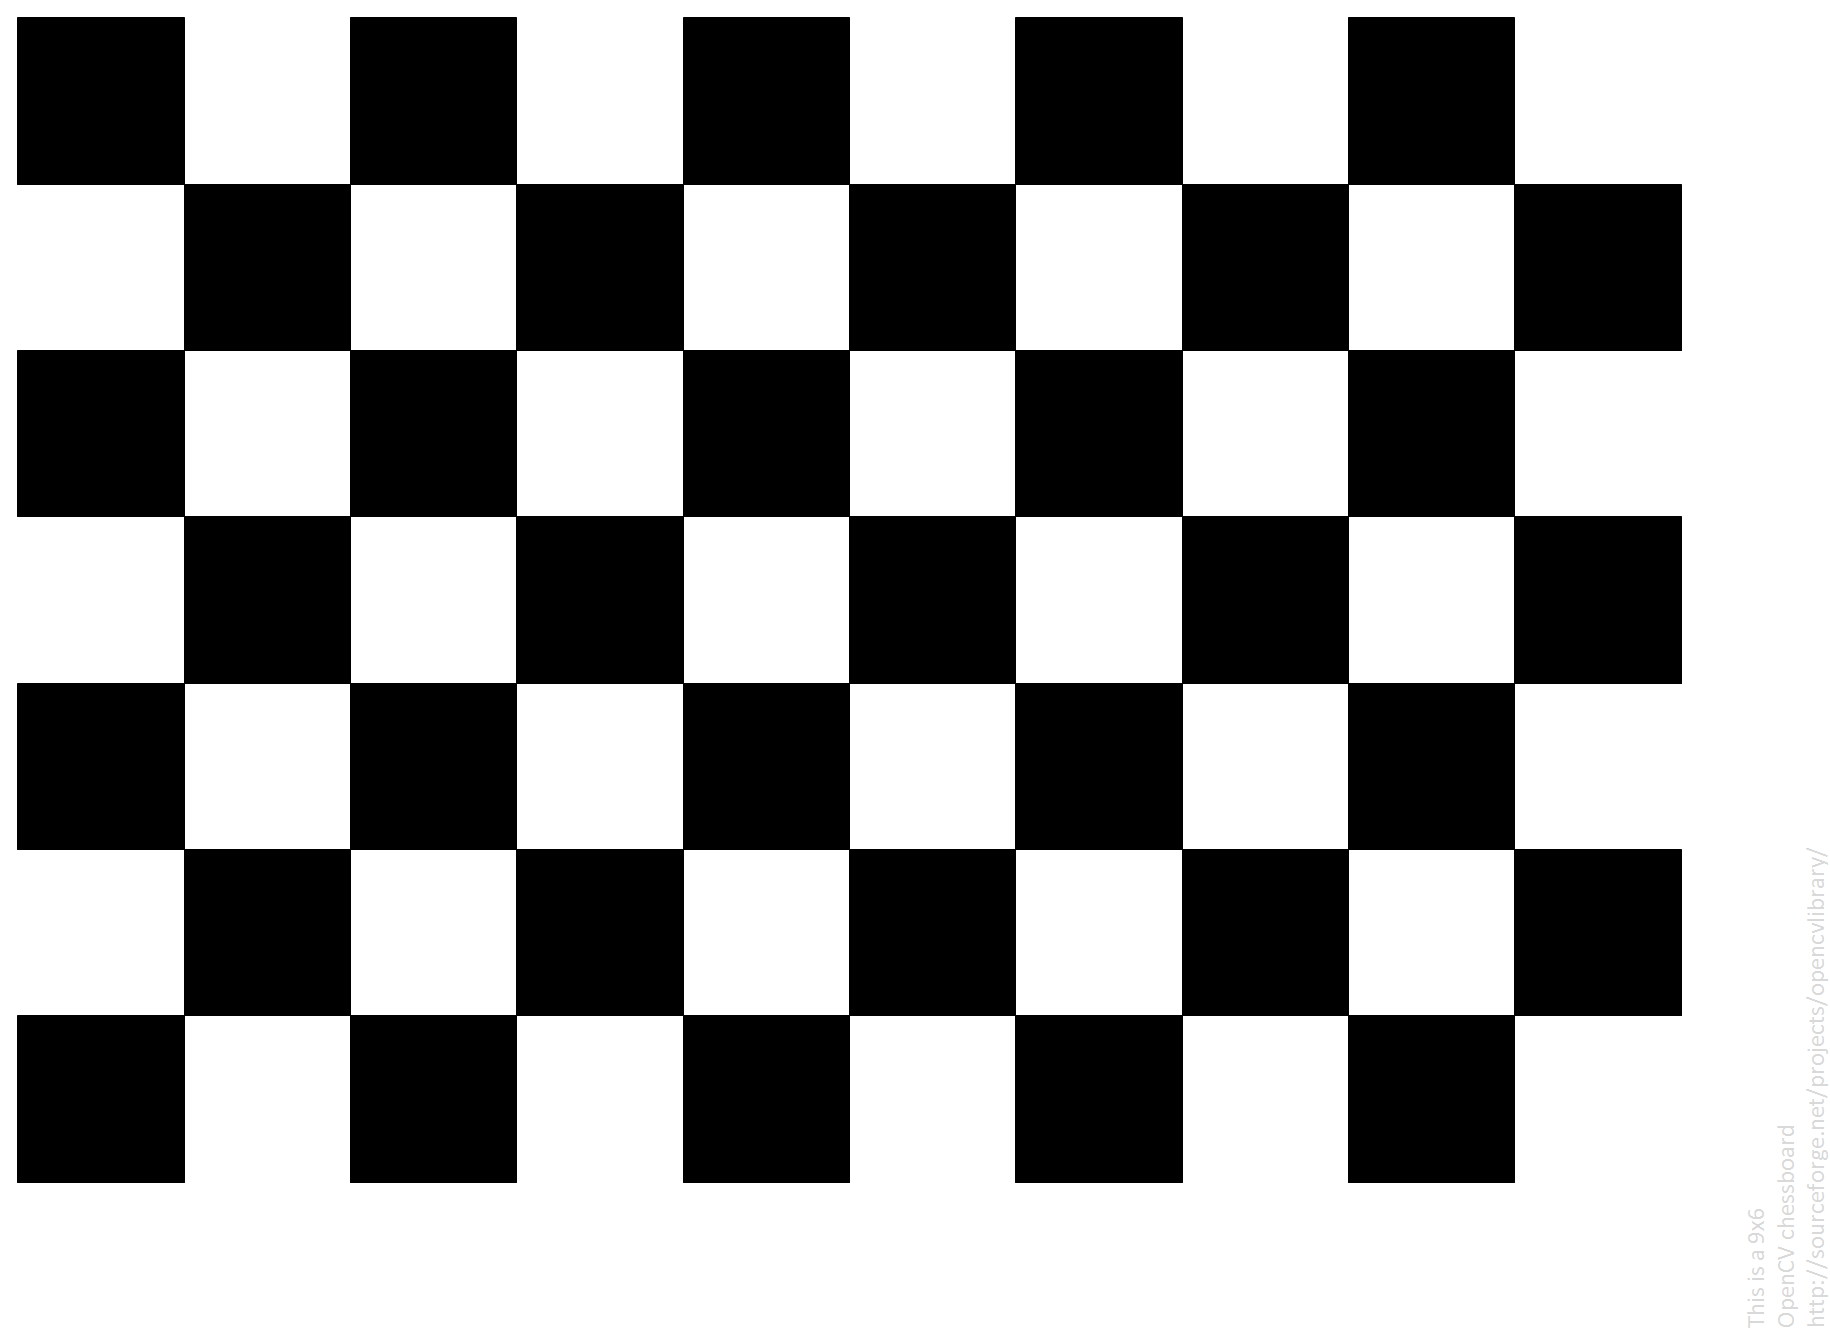
\includegraphics[width= \textwidth]{Imagens/figura3-3E3-12.png}
	\caption{Exemplo de padrão utilizado para a calibração}
	\label{fig3:12}
\end{figure}


Esse padrão por exemplo tem 10x7 casas, no entanto suas linhas são 9x6. Logo o parâmetro \texttt{--size} deve ser 9x6.
O parâmetro \texttt{--square} é o tamanho real do lado das casas do tabuleiro que imprimimos em metros. O comando acima indica que cada casa do tabuleiro possui 0,108 metros ou 10,8 centímetros. É recomendado que o usuário que reproduza estes passos use uma régua para medir o seu tabuleiro.
Após executar o comando, a janela de calibração será aberta, como mostra a figura 3.13:

\begin{figure}[H]
	\centering
		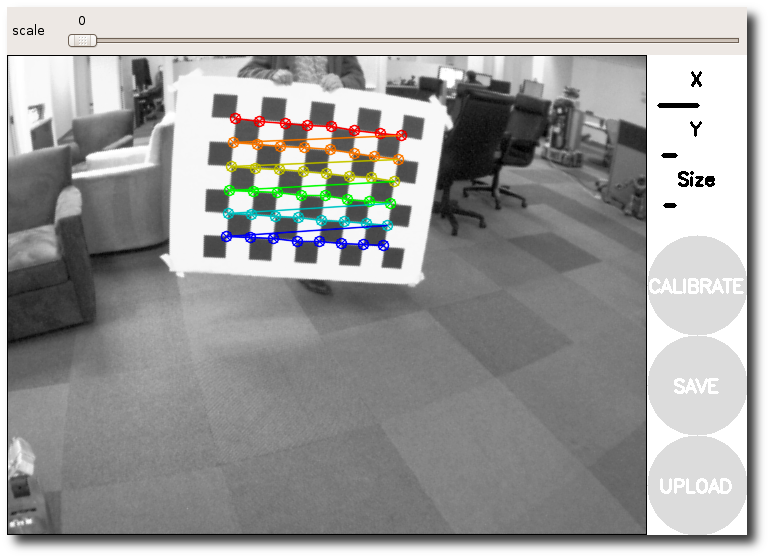
\includegraphics[width= \textwidth]{Imagens/figura3-13.png}
	\caption{Janela de configuração reconhecendo do tabuleiro}
	\label{fig3:13}
\end{figure}

\subsection{Movendo o tabuleiro}

Para se obter uma boa calibração é necessário mover o tabuleiro pelo quadro da câmera de modo que:

\begin{itemize}
	\item{O tabuleiro se encontre nas partes esquerda, direita, superior e inferior do campo de vista da câmera.}
	\begin{itemize}
		\item{Barra X - Campo de vista esquerda/direita.}
		\item{Barra Y - Campo de vista topo/baixo.}
		\item{Barra \textit{Size} - Aproximando/Afastando e Rotação da câmera.}
	\end{itemize}
	\item{O tabuleiro preencha todo o campo de vista.}
	\item{O tabuleiro inclinado para a esquerda,direita,topo,baixo (Barra \textit{Skew})}
\end{itemize}

A cada passo segure o tabuleiro até que que apareça na imagem o destaque do padrão.

\begin{figure}[H]
\minipage{0.32\textwidth}
  \caption{Desmonstração de posição para calibração \#1 \cite{Documentacao-CalibrateMonocularCamera}}\label{fig3:14}
  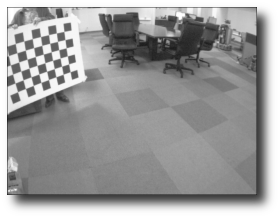
\includegraphics[width=\linewidth]{Imagens/figura3-14.png}
\endminipage\hfill
\minipage{0.32\textwidth}
  \caption{Desmonstração de posição para calibração \#2 \cite{Documentacao-CalibrateMonocularCamera}}\label{fig3:15}
  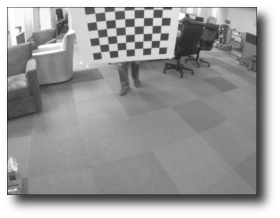
\includegraphics[width=\linewidth]{Imagens/figura3-15.png}
\endminipage\hfill
\minipage{0.32\textwidth}
  \caption{Desmonstração de posição para calibração \#3 \cite{Documentacao-CalibrateMonocularCamera}}\label{fig3:16}
  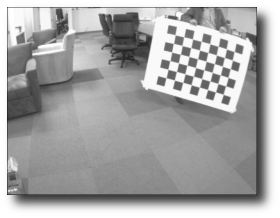
\includegraphics[width=\linewidth]{Imagens/figura3-16.png}
\endminipage
\end{figure}

\begin{figure}[H]
\minipage{0.32\textwidth}
  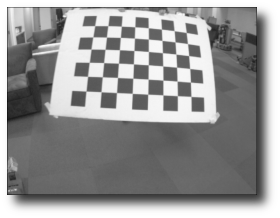
\includegraphics[width=\linewidth]{Imagens/figura3-17.png}
  \caption{Desmonstração de posição para calibração \#4 \cite{Documentacao-CalibrateMonocularCamera}}\label{fig3:17}
\endminipage\hfill
\minipage{0.32\textwidth}
  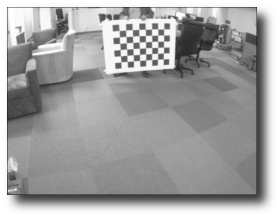
\includegraphics[width=\linewidth]{Imagens/figura3-18.png}
  \caption{Desmonstração de posição para calibração \#5 \cite{Documentacao-CalibrateMonocularCamera}}\label{fig3:18}
\endminipage\hfill
\minipage{0.32\textwidth}
  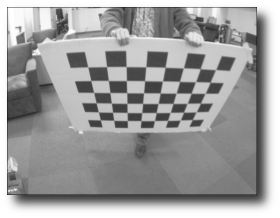
\includegraphics[width=\linewidth]{Imagens/figura3-19.png}
  \caption{Desmonstração de posição para calibração \#6 \cite{Documentacao-CalibrateMonocularCamera}}\label{fig3:19}
\endminipage
\end{figure}

Ao mover o tabuleiro, podem ser percebidas 4 Barras: X,Y,\textit{Size},\textit{Skew}; na barra lateral que aumentam de tamanho conforme ele vai capturando amostras. Quando o botão \textit{CALIBRATE} estiver iluminado quer dizer que há dados suficientes para calibrar. Um clique no botão inicia o processo de calibração.
A calibração dura em média um minuto. A janela estará cinza e inativa durante esse tempo. Isso indica que a calibração está ocorrendo e o programa não travou, bastando apenas aguardar.

\subsection{Resultados da calibração}

Depois de concluída a calibração os resultados dessa calibração podem ser vistos no terminal como demonstra a listagem \ref{tb:5}. Os valores poderão diferir dos apresentados, dependendo da câmera utilizada:


%{\setlength{\parindent}{0cm}
\begin{table}[H]\label{tb:5}
\begin{tabular}{| p{\textwidth}|}
\hline
\textcolor{orange}{\texttt{D = [-0.33758562758914146, 0.11161239414304096, -0.00021819272592442094, -3.029195446330518e-05]}}\\
\textcolor{orange}{\texttt{K = [430.21554970319971, 0.0, 306.6913434743704, 0.0, 430.53169252696676, 227.22480030078816, 0.0, 0.0, 1.0]}}\\
\texttt{R = [1.0, 0.0, 0.0, 0.0, 1.0, 0.0, 0.0, 0.0, 1.0]}\\
\texttt{P = [1.0, 0.0, 0.0, 0.0, 0.0, 1.0, 0.0, 0.0, 0.0, 0.0, 1.0, 0.0]}\\
 \texttt{\# oST version 5.0 parameters}\\
\\
 \texttt{[image]}\\
\\
\textcolor{orange}{\texttt{width}}\\
\textcolor{orange}{\texttt{640}}\\
\\
\textcolor{orange}{\texttt{height}}\\
\textcolor{orange}{\texttt{480}}\\
\\
 \texttt{[narrow\_stereo/left]}\\
\\
\texttt{camera matrix}\\
\texttt{430.215550 0.000000 306.691343}\\
\texttt{0.000000 430.531693 227.224800}\\
\texttt{0.000000 0.000000 1.000000}\\
\\
 \texttt{distortion}\\
 \texttt{-0.337586 0.111612 -0.000218 -0.000030 0.0000}\\
\\
 \texttt{rectification}\\
 \texttt{1.000000 0.000000 0.000000}\\
 \texttt{0.000000 1.000000 0.000000}\\
 \texttt{0.000000 0.000000 1.000000}\\
\\
 \texttt{projection}\\
 \texttt{1.000000 0.000000 0.000000 0.000000}\\
\\
 \texttt{0.000000 1.000000 0.000000 0.000000}\\
 \texttt{0.000000 0.000000 1.000000 0.000000}\\
\hline
\end{tabular}
\caption{Resultados da calibração impressos no console}
\end{table}

%}


 
Os valores destacados serão utilizados em breve. Uma calibração bem sucedida resultará em linhas retas no mundo real aparecerem como linhas retas na imagem corrigida. Uma calibração falha normalmente resulta em imagens em branco, irreconhecíveis ou que não preservam as linhas retas.
Após uma calibração bem sucedida pode-se ajustar o \textit{slider} \textit{SCALE} no topo da janela de calibração para mudar o tamanho da imagem retificada. Uma escala de 0.0 significa que a imagem está formatada de modo que os \textit{pixels} pretos criados para a preencher os espaços deixados pelos \textit{pixels} movidos não estejam presentes. A imagem não terá as curvas pretas de correção mas alguns \textit{pixels} da imagem original serão descartados. A escala de 1.0 significa que todos os \textit{pixels} da imagem original são visíveis mas a imagem corrigida tem bordas pretas onde não há \textit{pixels} de entrada da imagem original.
Se a calibração for satisfatória, o botão \textit{COMMIT} deve ser clicado para enviar os parâmetros de calibração para o armazenamento permanente. A \textit{GUI} fechará e a seguinte mensagem será impressa no console \textit{“writing calibration data to...”}.

\subsection{Criação do arquivo de calibração}

Do modo que está, o \textit{LSD-SLAM} irá utilizar a calibração salva, no entanto é interessante criar um arquivo de configuração para ser facilmente reutilizado caso se queira usar essa configuração em outra máquina ou salvar a calibração em um local mais seguro. Esse arquivo de calibração também é importante pois o \texttt{dataset\_slam} necessita dele para executar, ou seja, ele não usa a calibração salva pelo calibrador em disco. Na seção anterior foram destacadas em laranja alguns valores:

%{\setlength{\parindent}{0cm}
\begin{table}[H]\label{tb:6}
\begin{tabular}{| p{\textwidth}|}
\hline
\texttt{D = [\textcolor{orange}{-0.33758562758914146}, \textcolor{orange}{0.11161239414304096}, \textcolor{orange}{-0.00021819272592442094}, \textcolor{orange}{-3.029195446330518e-05}]}\\
\texttt{K = [\textcolor{red}{430.21554970319971}, 0.0, \textcolor{purple}{306.6913434743704}, 0.0, \textcolor{blue}{430.53169252696676}, \textcolor{brown}{227.22480030078816}, 0.0, 0.0, 1.0]}\\
\\
\texttt{width}\\
\texttt{\textcolor{OliveGreen}{640}}\\
\\
\texttt{height}\\
\texttt{\textcolor{WildStrawberry}{480}}\\
\\
\hline
\end{tabular}
\caption{Informações relevantes extraídas da listagem \ref{tb:5}}
\end{table}


Esses valores serão usados para compor o arquivo. Em um novo documento de texto insira o seguinte modelo:

\begin{table}[H]\label{tb:7}
\begin{tabular}{| p{\textwidth}|}
\hline
\texttt{\textcolor{red}{fx}/\textcolor{OliveGreen}{width} \textcolor{blue}{fy}/\textcolor{WildStrawberry}{height} \textcolor{purple}{cx}/\textcolor{OliveGreen}{width} \textcolor{brown}{cy}/\textcolor{WildStrawberry}{height} \textcolor{orange}{d}}\\
\texttt{\textcolor{OliveGreen}{in\_width} \textcolor{WildStrawberry}{in\_height}}\\
\texttt{"crop" / "full" / "none"}\\
\texttt{\textcolor{OliveGreen}{out\_width} \textcolor{WildStrawberry}{out\_height}}\\
\hline
\end{tabular}
\caption{Modelo de arquivo de configuração com legenda}
\end{table}

Dessa forma deve-se fazer os cálculos substituindo os valores do modelo com os da suas cores respondentes acima, quanto mais casas decimais, melhor, pois isso potencialmente reduz o erro. Na terceira linha:

\begin{description}
\item[\texttt{crop}]{Corta a imagem para o tamanho máximo enquanto inclui apenas \textit{pixels} válidos.}
\item[\texttt{full}]{Não corta a imagem mas pode incluir \textit{pixels} inválidos}
\item[\texttt{none}]{Não realiza a operação de correção de distorção radial}
\end{description}

Recomenda-se o uso do valor \texttt{crop}. O resultado final deve ficar à listagem \ref{tb:8}:

\begin{table}[H]\label{tb:8}
\begin{tabular}{| p{\textwidth}|}
\hline
\texttt{
0,672211796411249546875 0,89694102609784741666666666666667 0,47920522417870375 0,473385000626642 -0.33758562758914146 0.11161239414304096 -0.00021819272592442094 -0.00003.029195446330518}\\
\texttt{640 480}\\
\texttt{crop}\\
\texttt{640 480}\\
\hline
\end{tabular}
\caption{Exemplo de arquivo de configuração final}
\end{table}

Uma observação é que ao inserir os resultados no arquivo, deve-se certificar que o ponto flutuante é ‘.’(ponto) e não ‘,’(vírgula) pois isso fará com que o arquivo não funcione corretamente. Depois disso arquivo deve ser salvo como \texttt{nome\_do\_arquivo\_de\_calibração.cfg} e estará pronto para ser usado. Se estiver usando um arquivo de calibração do \textit{OpenCV}, que foi o usado no \textit{PhotoGuide}, a transformação é similar ao resultado da calibração do \textit{LSD-SLAM}. Considerando a seguinte saída da calibração do \textit{OpenCV}:

\begin{table}[H]\label{tb:9}
\begin{tabular}{| p{\textwidth}|}
\hline
\texttt{<Camera\_Matrix type\_id="opencv-matrix">}\\
\texttt{<rows>3</rows>}\\
\texttt{<cols>3</cols>}\\
\texttt{<dt>d</dt>}\\
\texttt{<data>}\\
\texttt{ \textcolor{red}{6.5746697944293521e+002} 0. \textcolor{purple}{3.1950000000000000e+002}}\\
\texttt{ 0. \textcolor{blue}{6.5746697944293521e+002} \textcolor{brown}{2.3950000000000000e+002}}\
\texttt{ 0. 0. 1.}\\
\texttt{</data></Camera\_Matrix>}\\
\texttt{<Distortion\_Coefficients type\_id="opencv-matrix">}\\
\texttt{<rows>5</rows>}\\
\texttt{<cols>1</cols>}\\
\texttt{<dt>d</dt>}\\
\texttt{<data>}\\
\texttt{ \textcolor{orange}{-4.1802327176423804e-001 5.0715244063187526e-001 0. 0.} -5.7843597214487474e-001</data></Distortion\_Coefficients>}\\
 \hline
\end{tabular}
\caption{Exemplo de arquivo de calibração do \textit{OpenCV}}
\end{table}

Deve ser convertido para um arquivo no formato \textit{.cfg} de modo que:

\begin{table}[H]\label{tb:10}
\begin{tabular}{| p{\textwidth}|}
\hline
\texttt{\textcolor{red}{fx} \textcolor{purple}{fy} \textcolor{blue}{cx} \textcolor{brown}{cy} \textcolor{orange}{k1 k2 p1 p2}}\\
\texttt{640 480}\\
\texttt{"crop" / "full" / "none"}\\
\texttt{640 480}\\
 \hline
\end{tabular}
\caption{Modelo de arquivo de configuração usando a calibração do \textit{OpenCV}}
\end{table}

Lembrando que o \textit{LSD-SLAM} não suporta notação científica, nesse exemplo o arquivo final ficará dessa forma:

\begin{table}[H]\label{tb:11}
\begin{tabular}{| p{\textwidth}|}
\hline
\texttt{0.065746697944293521 0.03195 0.065746697944293521 0.02395 -0.41802327176423804 0.50715244063187526 0 0}\\
\texttt{640 480}\\
\texttt{crop}\\
\texttt{640 480}\\
 \hline
\end{tabular}
\caption{Exemplo de arquivo de configuração final usando a calibração do \textit{OpenCV}}
\end{table}

\section{Utilização da ferramenta}

Com a câmera calibrada pode-se agora começar a usar de fato a ferramenta. O \textit{LSD-SLAM} é dividido em dois pacotes \textit{ROS}, \texttt{lsd\_slam\_core} e \texttt{lsd\_slam\_viewer}. \texttt{lsd\_slam\_core} contém o sistema \textit{SLAM} completo, enquanto o \texttt{lsd\_slam\_viewer} é opcionalmente usado para a visualização 3D.
Para inicializar o sistema do \textit{LSD-SLAM} é o suficiente começar com um primeiro quadro-chave com uma imagem de alta variância de profundidade e grande quantidade de detalhes. Com suficientes movimentos translacionais da câmera nos primeiros segundos o algoritmo “trava” em uma certa configuração, e após algumas propagações de quadros-chaves ela converge para a configuração correta de profundidade.

\subsection{\texttt{lsd\_slam\_viewer} - Visualizador 3D}

O visualizador, além de ser usado para visualizar, também pode ser usado para exportar a nuvem de pontos como .ply. Para abrir o visualizador, o seguinte comando é executado:

\begin{table}[H]\label{tb:12}
\begin{tabular}{| p{\textwidth}|}
\hline
\texttt{rosrun lsd\_slam\_viewer viewer}\\
\hline
\end{tabular}
\caption{Comando para executar o visualizador 3D}
\end{table}

Esse comando irá abrir a tela de \textit{PointCloudViewer}, nela é possível ver em tempo real como está a reconstrução do ambiente. Também é possível gravar e reproduzir a saída gerada pelas trajetórias usando respectivamente os comandos para gravar e reproduzir:

\begin{table}[H]\label{tb:13}
\begin{tabular}{| p{\textwidth}|}
\hline
\texttt{rosbag record /lsd\_slam/graph /lsd\_slam/keyframes /lsd\_slam/liveframes -o file\_pc.bag}\\
\texttt{rosbag play file\_pc.bag}\\
\hline
\end{tabular}
\caption{Dois comandos, um para gravar e outro para reproduzir a saída do visualizador no formato .bag}
\end{table}

Não haverá necessidade de reiniciar o visualizador, ele irá reiniciar automaticamente ao se carregar uma entrada diferente. Alguns atalhos úteis para usar na janela:

\begin{description}
	\item[r :]{Reset, limpa todos os dados mostrados.}
	\item[w :]{Imprime o número de total de pontos, pontos sendo mostrados no momento, \textit{Keyframes} (Quadros-chave) e restrições no console.}
	\item[p :]{Escreve os pontos atualmente mostras como nuvem de pontos para o arquivo: lsd\_slam\_viewer/pc.ply, que pode ser aberto, por exemplo, no \textit{Meshlab}. Use  em combinação com o \textit{sparsityFactor}  para reduzir o número de pontos escritos.}
\end{description}	

\subsection{Obtendo o mapa 3D usando o \texttt{live\_slam}}

Para visualizar a nuvem de pontos em tempo real, usando uma câmera, o seguinte comando deve ser executado:

\begin{table}[H]\label{tb:14}
\begin{tabular}{| p{\textwidth}|}
\hline
\texttt{rosrun lsd\_slam\_core live\_slam /image:=\textcolor{red}{usb\_cam/image\_raw} /camera\_info:=\textcolor{red}{usb\_cam}}\\
\hline
\end{tabular}
\caption{Comando para executar o \texttt{live\_slam} com calibração salva no \textit{ROS}}
\end{table}

Os parâmetros destacados em vermelhos estão preenchidos com os que o usuário configurou em sua máquina, nesse trabalho optamos pelas nomenclaturas padrão de instalação. Ao se usar esse comando, apenas as dimensões da imagem e a matriz $K$ das mensagens de \texttt{camera\_info} serão usadas, isto é, o vídeo tem que estar corrigido.

Alternativamente, pode-se especificar um arquivo de calibração usando o seguinte comando:

\begin{table}[H]\label{tb:15}
\begin{tabular}{| p{\textwidth}|}
\hline
\texttt{rosrun lsd\_slam\_core live\_slam /image:=\textcolor{red}{usb\_cam/image\_raw} \_calib:=\textcolor{blue}{/caminho/para/seu/arquivodeccalibracao}}\\
\hline
\end{tabular}
\caption{Comando para executar o \texttt{live\_slam} com arquivo de calibração externo}
\end{table}

Novamente, o texto em vermelho corresponde ao que foi configurado pelo usuário anteriormente. O texto \texttt{\textcolor{blue}{/caminho/para/seu/arquivodeccalibracao}} deve ser trocado para o caminho do arquivo de calibração criado.

As telas a seguir mostram exemplos da ferramenta rodando, durante a captura dessas telas as nuvem de pontos não foi rotacionada portanto está na sua posição inicial que é de cabeça para baixo. 

\begin{figure}[H]
	\centering
		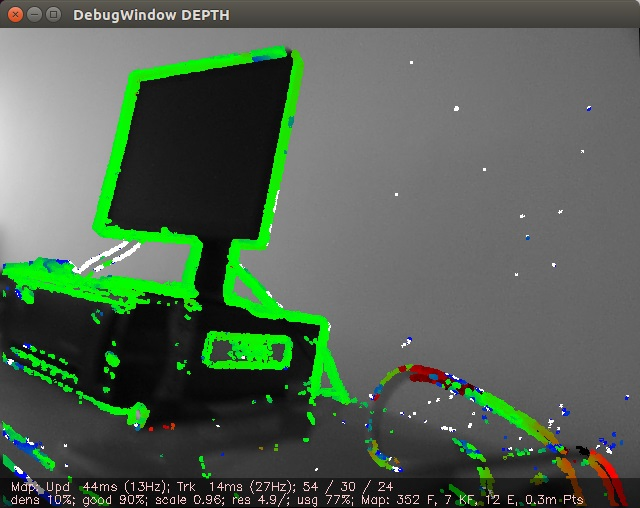
\includegraphics[width= \textwidth]{Imagens/figura3-20.jpg}
	\caption{\textit{DebugWindow DEPTH} do \texttt{live\_slam} \#1}
	\label{fig3:20}
\end{figure}

\begin{figure}[H]
	\centering
		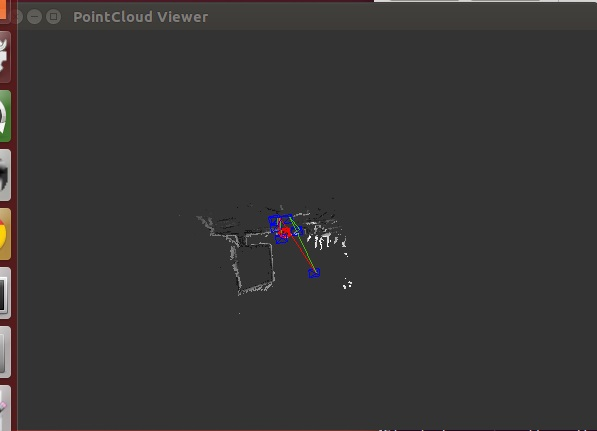
\includegraphics[width= \textwidth]{Imagens/figura3-21.jpg}
	\caption{\textit{PointCloud} referente à figura \ref{fig3:20}}
	\label{fig3:21}
\end{figure}

\begin{figure}[H]
	\centering
		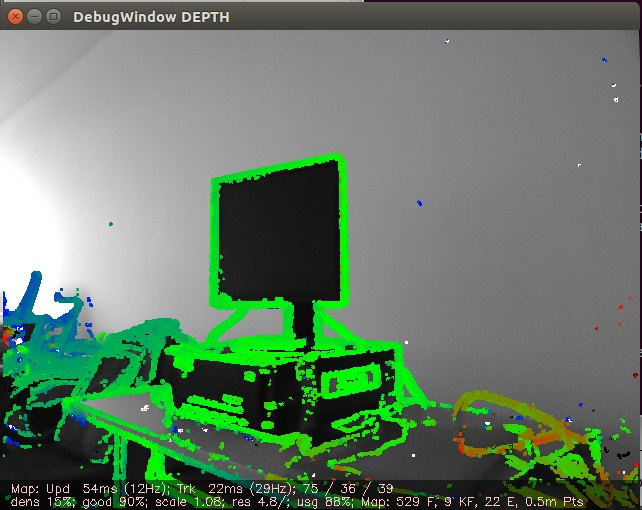
\includegraphics[width= \textwidth]{Imagens/figura3-22.jpg}
	\caption{\textit{DebugWindow DEPTH} do\texttt{ live\_slam} \#2}
	\label{fig3:22}
\end{figure}

\begin{figure}[H]
	\centering
		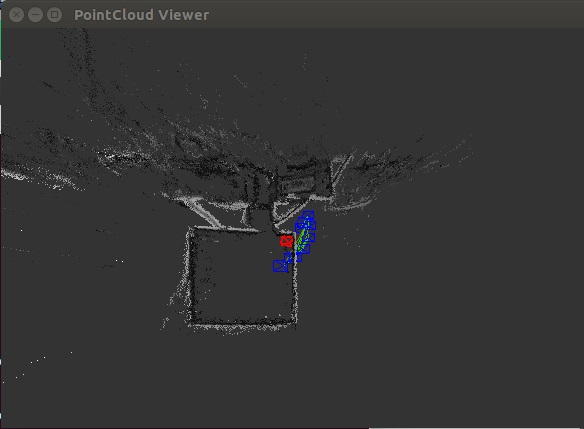
\includegraphics[width= \textwidth]{Imagens/figura3-23.jpg}
	\caption{\textit{PointCloud} referente à figura \ref{fig3:22}}
	\label{fig3:23}
\end{figure}

\begin{figure}[H]
	\centering
		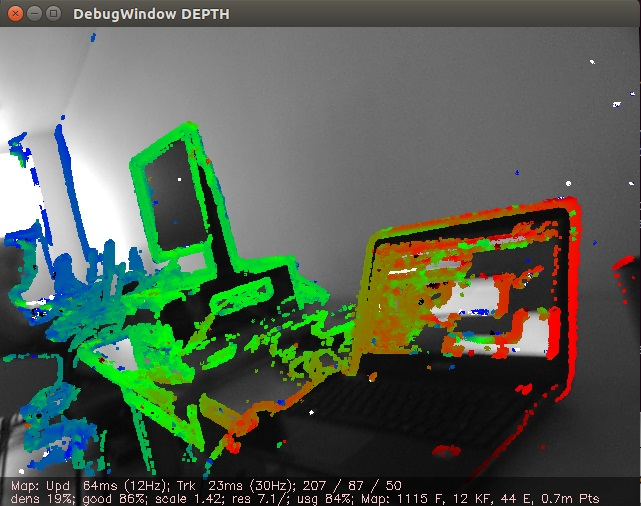
\includegraphics[width= \textwidth]{Imagens/figura3-24.jpg}
	\caption{\textit{DebugWindow DEPTH} do \texttt{live\_slam} \#3}
	\label{fig3:24}
\end{figure}

\begin{figure}[H]
	\centering
		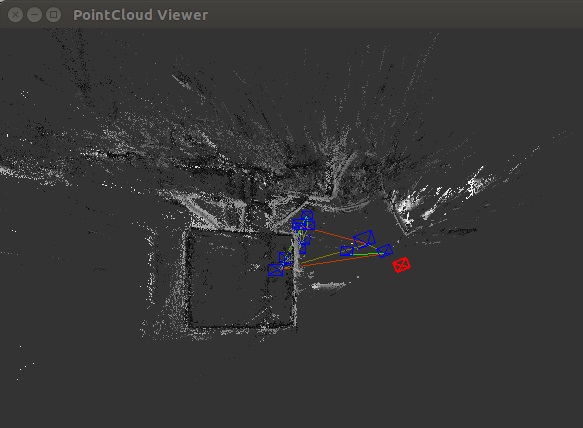
\includegraphics[width= \textwidth]{Imagens/figura3-25.jpg}
	\caption{\textit{PointCloud} referente à figura \ref{fig3:24}}
	\label{fig3:25}
\end{figure}

A saída do \texttt{lsd\_slam\_core} está sendo transferida para o visualizador na janela \textit{PointCloud Viewer} no formato de nuvem de pontos que podem ser rotacionados e observados em qualquer ângulo. A janela \textit{DebugWindow DEPTH} é a janela que oferece informações sobre a execução do algoritmo incluindo:

\begin{description}
	\item[Map upd :]{A taxa em que os quadros estão sendo computados.}
	\item[Trk :]{A taxa de quadros do \textit{dataset}/câmera.}
	\item[X/Y/Z :]{O terceiro parâmetro não possui identificação mas se encontra no formato X/Y/Z e significa rotação do quadro atual com o quadro original nos 3 eixos.}
	\item[Dens X\% :]{A densidade média dos pontos.}
	\item[Good X\% :]{ A quantidade de pontos pontos bons que podem ser utilizados pelo algoritmo, importante para verificar condições de distorção na imagem da câmera como: iluminação, foco, movimentação, taxa de bits insuficiente na compressão ou similaridade daquele quadro atual com os feitos anteriormente.}
	\item[Scale X\% :]{Escala entre os pontos.}
	\item{Número de pontos utilizados pelo algoritmo.}
	\item{Quadro atual.}
	\item{Numeração de quadro refinador por \textit{keyframe}.}
\end{description}

Além disso as cores representam o grau de proximidade de cada ponto à câmera. Pontos vermelhos são os mais próximos, pontos verdes estão à meia distância e pontos azuis são os mais distantes. Pontos e gradientes brancos foram reconhecidos pelo detecção de gradiente mas não conseguiu ser reconhecido em escala considerando o \textit{keyframe} atual, normalmente isso ocorre quando há uma diferença de escala inesperada como um objeto que se move ou se a iluminação ou foco da câmera atrapalhar no reconhecimento.

Essas informações são comuns tanto ao \texttt{live\_slam} quanto ao \texttt{dataset\_slam}. O método \texttt{live\_slam} se caracteriza por servir de teste do ambiente para se fazer o \textit{dataset}. Ele possui suas vantagens e desvantagens:

Vantagens:

\begin{itemize}
	\item{O funcionamento do algoritmo pode ser visto em tempo real.}
	\item{A condição de iluminação pode ser testada usando esse modo mais rapidamente.}
\end{itemize}

Desvantagens:

\begin{itemize}
	\item{É necessário utilizar em um computador portátil para que se possa mover com a câmera.}
	\item{A mobilidade enquanto se usa esse método é prejudicada.}
	\item{É mais difícil mudar os parâmetros enquanto roda o algoritmo.}
	\item{Baixa reproducibilidade.}
	\item{Alto consumo de recursos do computador.}
\end{itemize}	

Também é possível salvar o vídeo capturado usando o parâmetro do \texttt{lsd\_slam\_viewer} \textit{saveAllVideo}, no entanto essa operação é ainda mais custosa. Nas máquinas usadas para os testes, não foi possível usar essa opção.

\subsection{Obtendo o mapa 3D usando o \texttt{dataset\_slam}}

Para obter o mapa utilizando um \textit{dataset}, execute o seguinte comando:

\begin{table}[H]\label{tb:16}
\begin{tabular}{| p{\textwidth}|}
\hline
\texttt{rosrun lsd\_slam\_core dataset\_slam \_files:=/caminho/para/seu/dataset \_hz:=<hz> \_calib:=/caminho/para/seu/arquivodeccalibracao}\\
\hline
\end{tabular}
\caption{Comando para executar o \texttt{dataset\_slam} com um arquivo de calibração externo}
\end{table}

Troque \texttt{/caminho/para/seu/dataset} pelo caminho do seu \textit{dataset}, \texttt{<hz>} idealmente deverá ser trocado para 0, o que permite o rastreamento e mapeamento sequencial, mas haverá uma queda de desempenho do que a contrapartida em tempo real. Por fim, troque \texttt{/caminho/para}\texttt{/seu/arquivodeccalibracao} pelo caminho do seu arquivo de configuração resultante na seção 3.2.3.6. Segue abaixo algumas capturas de tela com o comando sendo executado:

\begin{figure}[H]
	\centering
		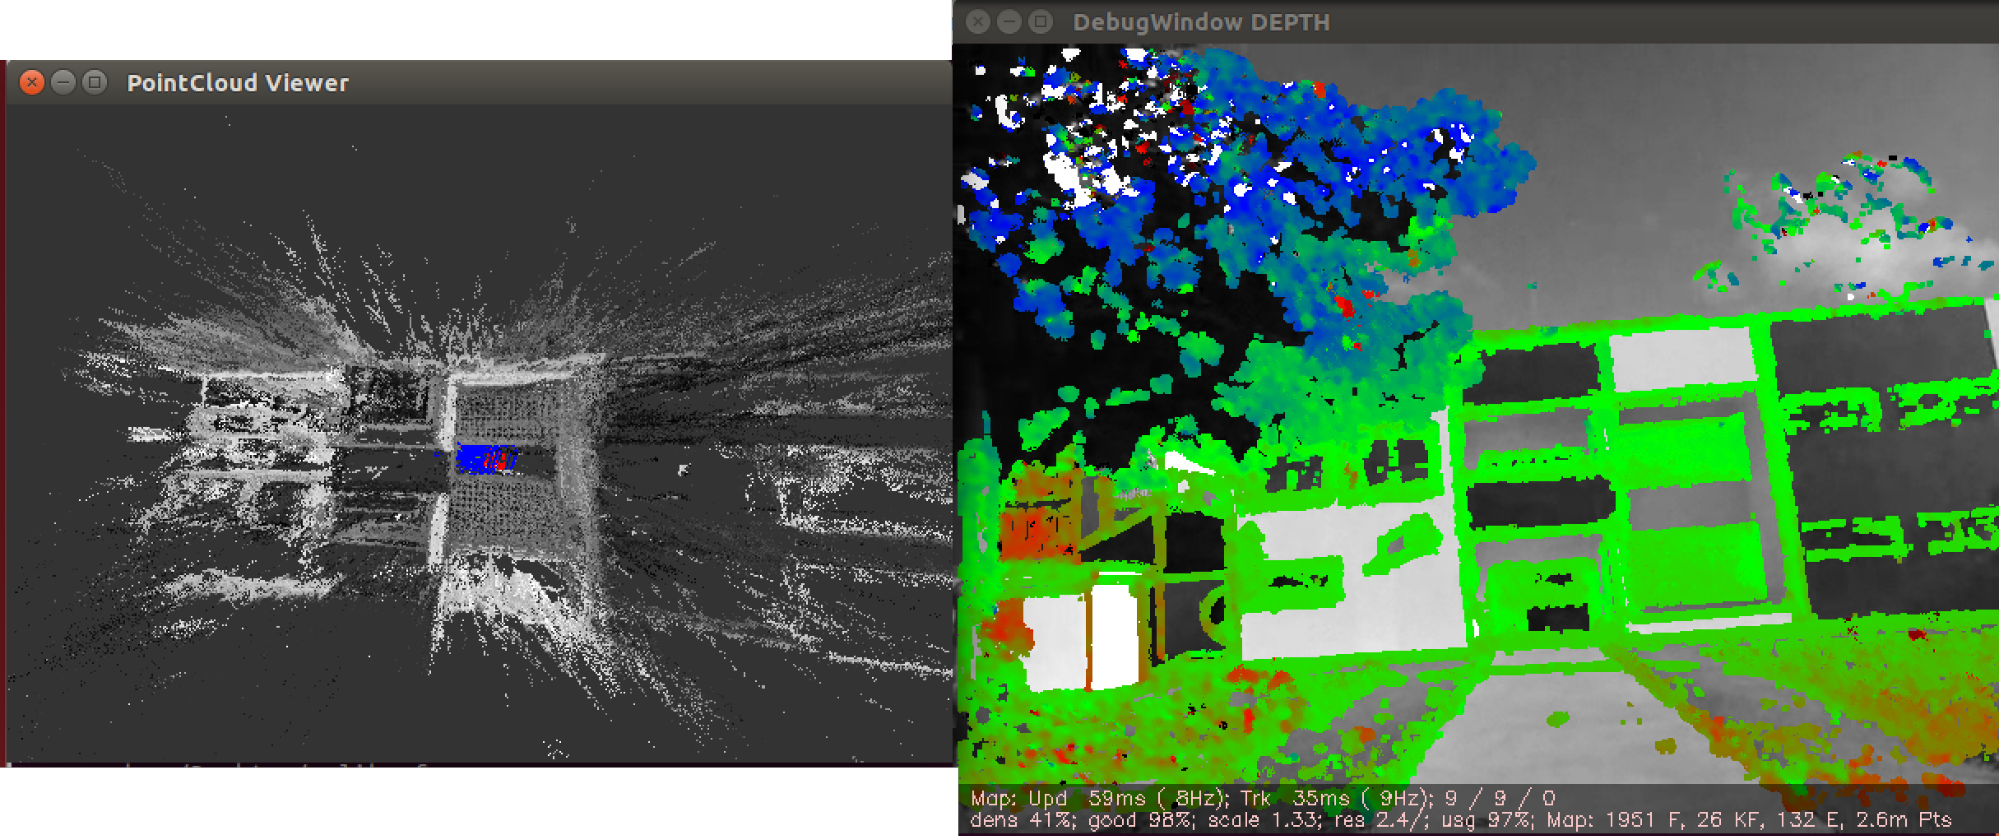
\includegraphics[width= \textwidth]{Imagens/figura3-26E3-27.png}
	\caption{\textit{PointCloud} e \textit{DebugWindow DEPTH} do \texttt{dataset\_slam} \#1}
	\label{fig3:26}
\end{figure}





\begin{figure}[H]
	\centering
		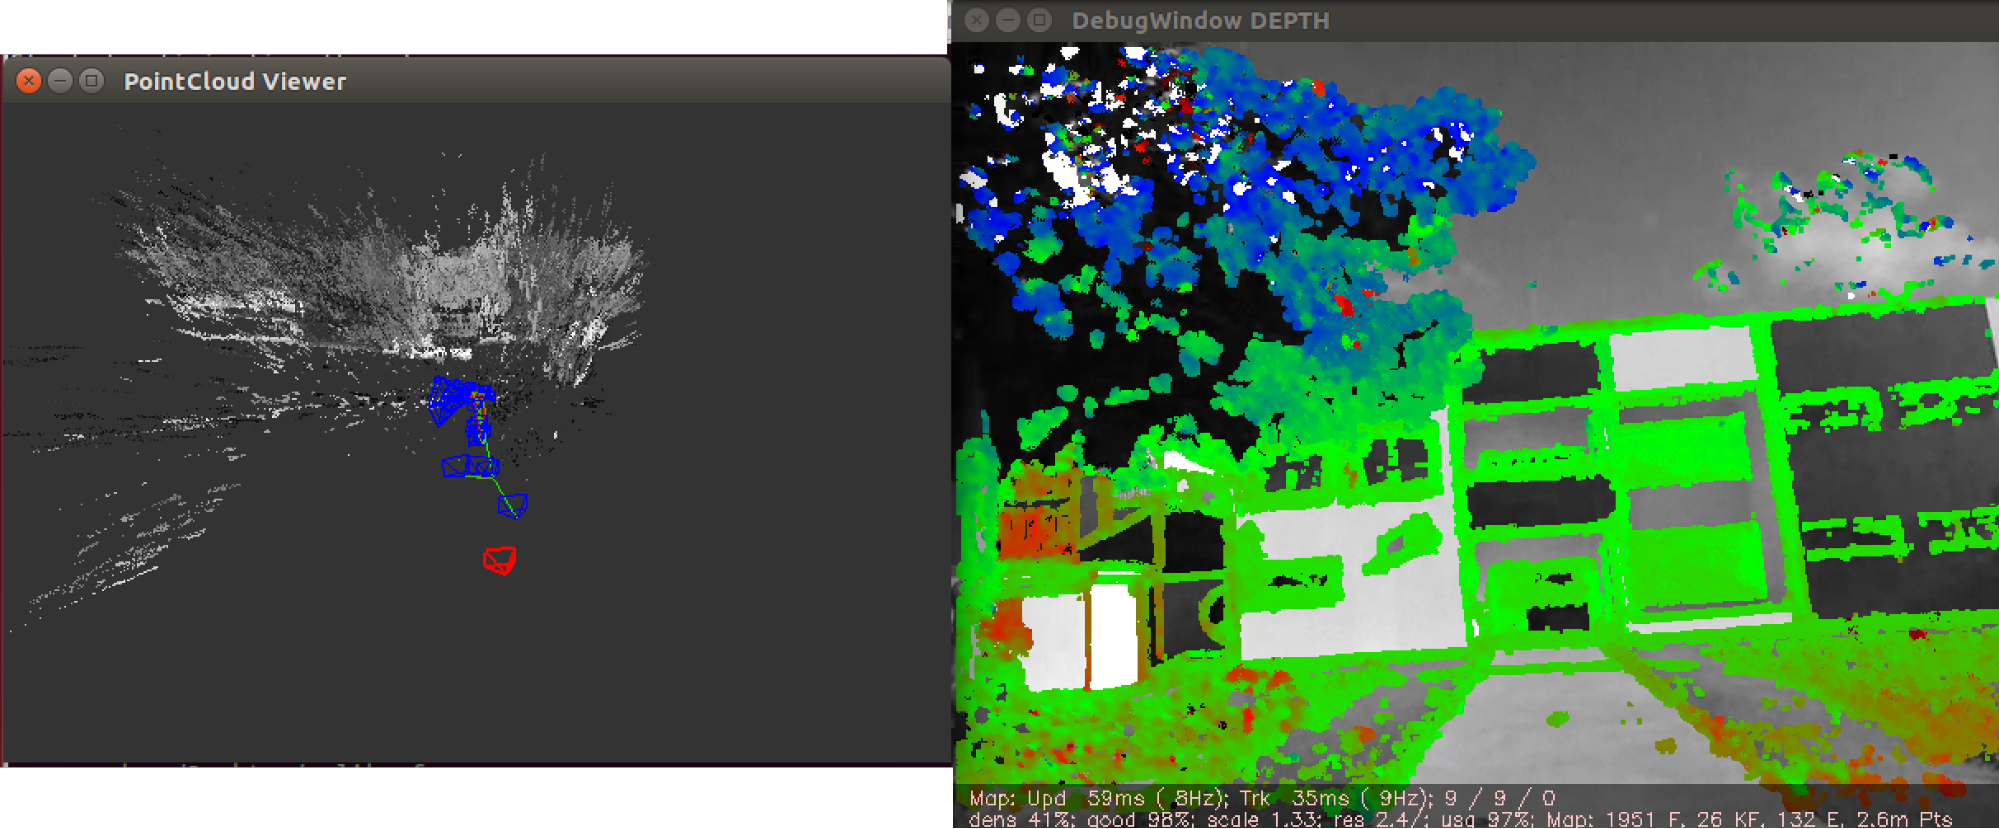
\includegraphics[width= \textwidth]{Imagens/figura3-28E3-29.png}
	\caption{\textit{PointCloud} e \textit{DebugWindow DEPTH} do \texttt{dataset\_slam} \#4}
	\label{fig3:27}
\end{figure}

É necessário também, dependendo do \textit{dataset} usado, um refinamento dos parâmetros de visualização e também da forma que o \texttt{lsd\_slam\_core} opera, pois com os parâmetros padrão é possível perceber que a grama em frente ao prédio atrapalhou a captura dos gradientes.

\subsection{Parâmetros \texttt{rqt\_reconfigure}}

Uma característica fundamental da ferramenta é a capacidade de modificar alguns parâmetros do algoritmo, esses parâmetros podem ser modificados usando a ferramenta \texttt{rqt\_reconfigure} que vem junto com o pacote do \textit{LSD-SLAM} que pode ser chamado usando o seguinte comando:

\begin{table}[H]\label{tb:17}
\begin{tabular}{| p{\textwidth}|}
\hline
\texttt{rosrun rqt\_reconfigure rqt\_reconfigure}\\
\hline
\end{tabular}
\caption{Comando para inicialização do \texttt{rqt\_reconfigure}}
\end{table}

E então será aberta uma janela com vários parâmetros dependendo de quais janelas do \textit{LSD-SLAM} estão abertas, isto é, o \texttt{lsd\_slam\_core} e o \texttt{lsd\_slam\_viewer}. Para cada uma das janelas os parâmetros podem ser modificados em tempo real. A figura 3.30 mostra alguns parâmetros de configuração.

\begin{figure}[H]
	\centering
		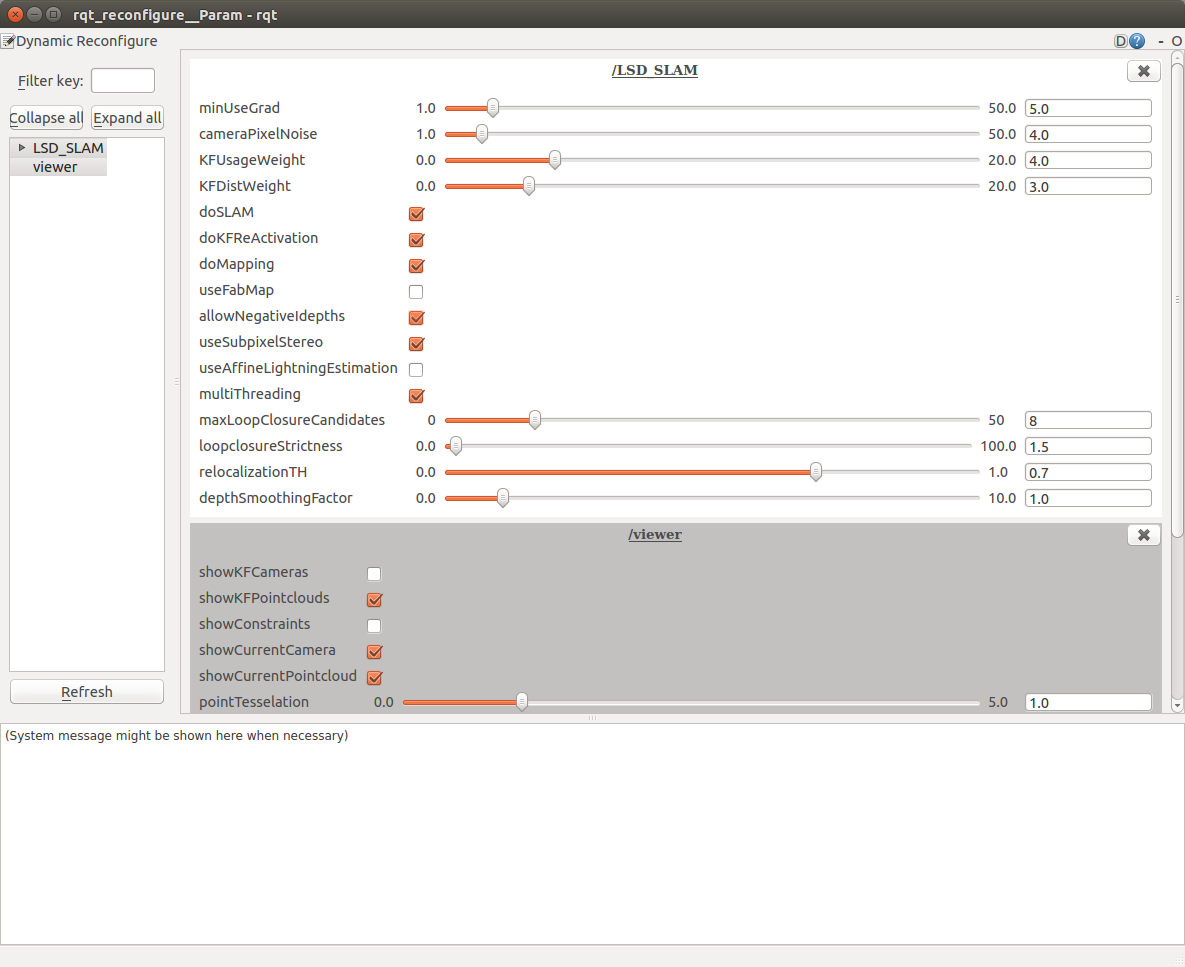
\includegraphics[width= \textwidth]{Imagens/figura3-30.png}
	\caption{Tela do \texttt{rqt\_reconfigure}}
	\label{fig3:28}
\end{figure}



\subsubsection{\textit{minUseGrad}}

Esse parâmetro indica a extensão mínima do gradiente para que o algoritmo o reconheça. Em outras palavras, quanto maior esse valor, mais restritiva será a captura de gradientes. Diminuindo esse parâmetro, gradientes pequenos como texturas irregulares, grama e outros gradientes não uniformes serão reconhecidos. Deve-se analisar cuidadosamente o quanto do ambiente deseja-se capturar e ajustar esse parâmetro de acordo, assim como o exemplo a seguir:

\begin{figure}[H]
	\centering
		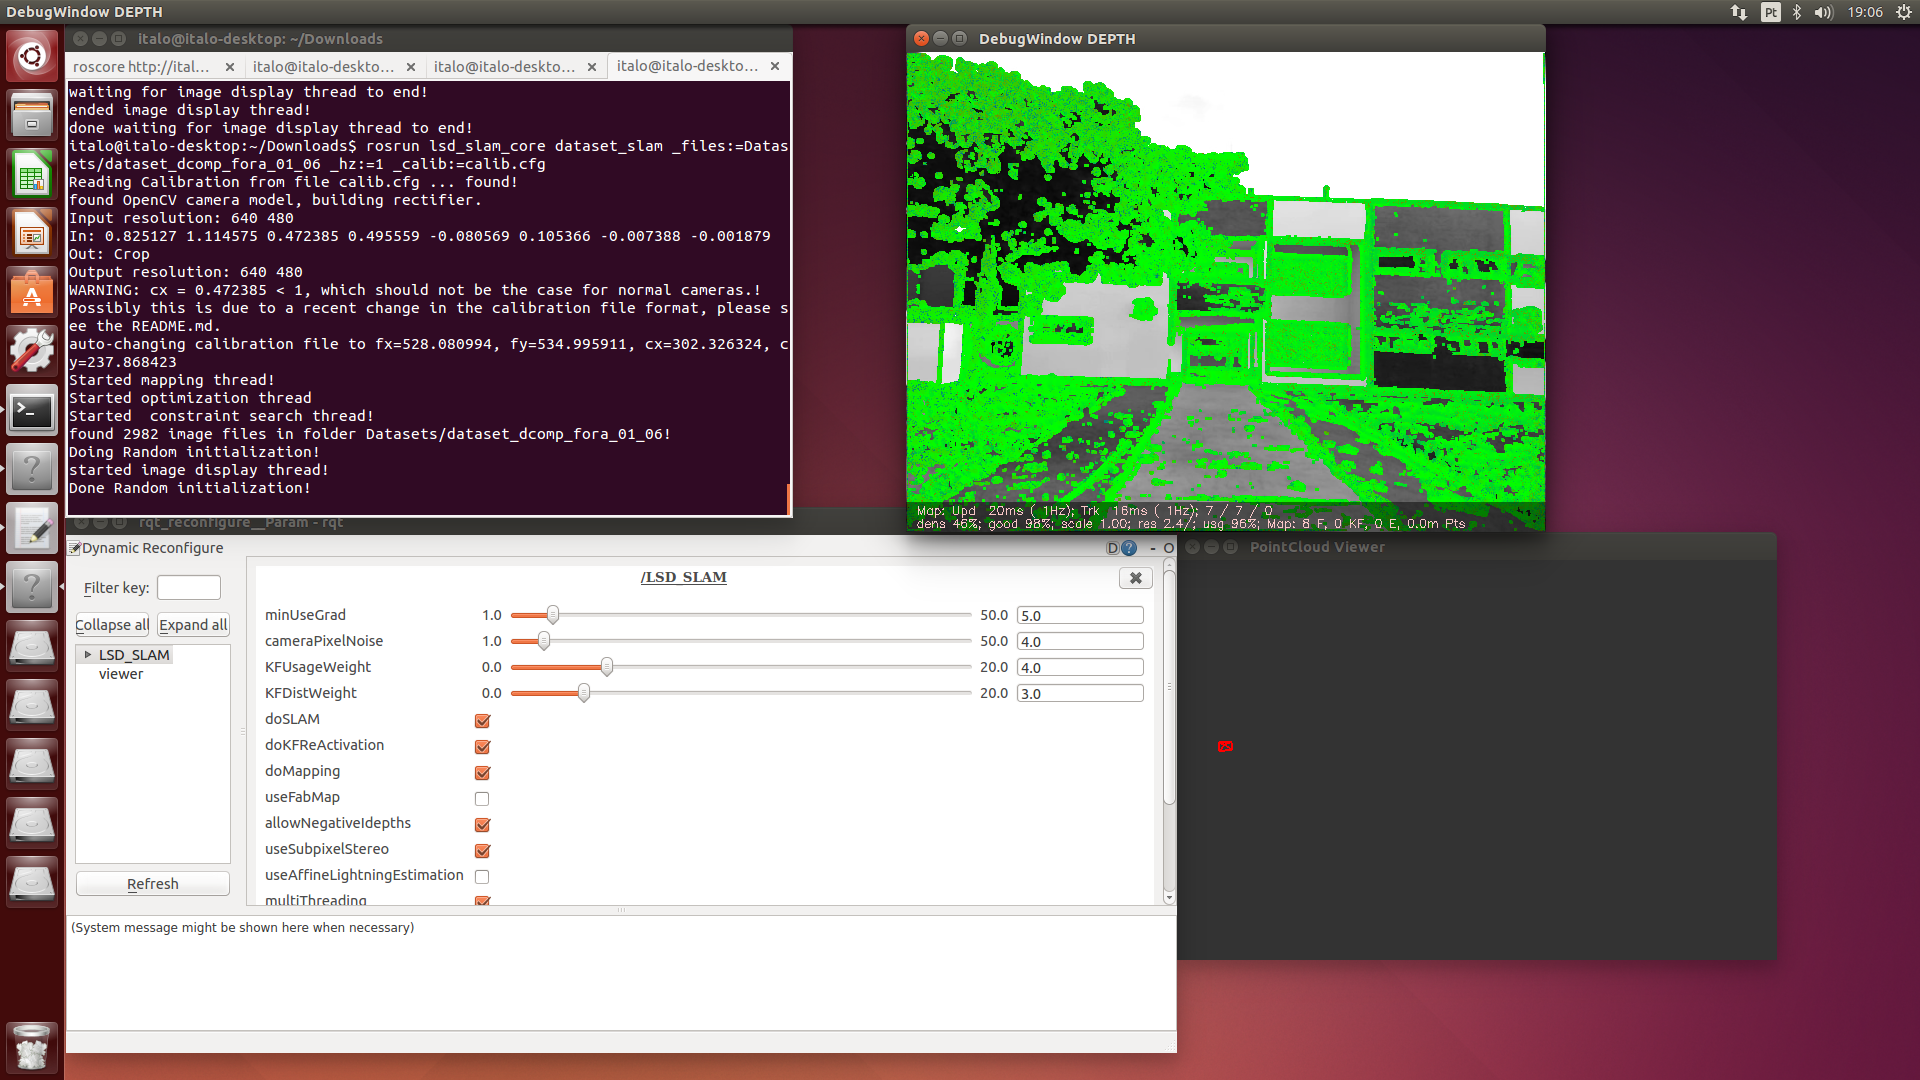
\includegraphics[width= \textwidth]{Imagens/figura3-31.png}
	\caption{\textit{minUseGrad} no seu valor padrão de 5.0}
	\label{fig3:29}
\end{figure}

\begin{figure}[H]
	\centering
		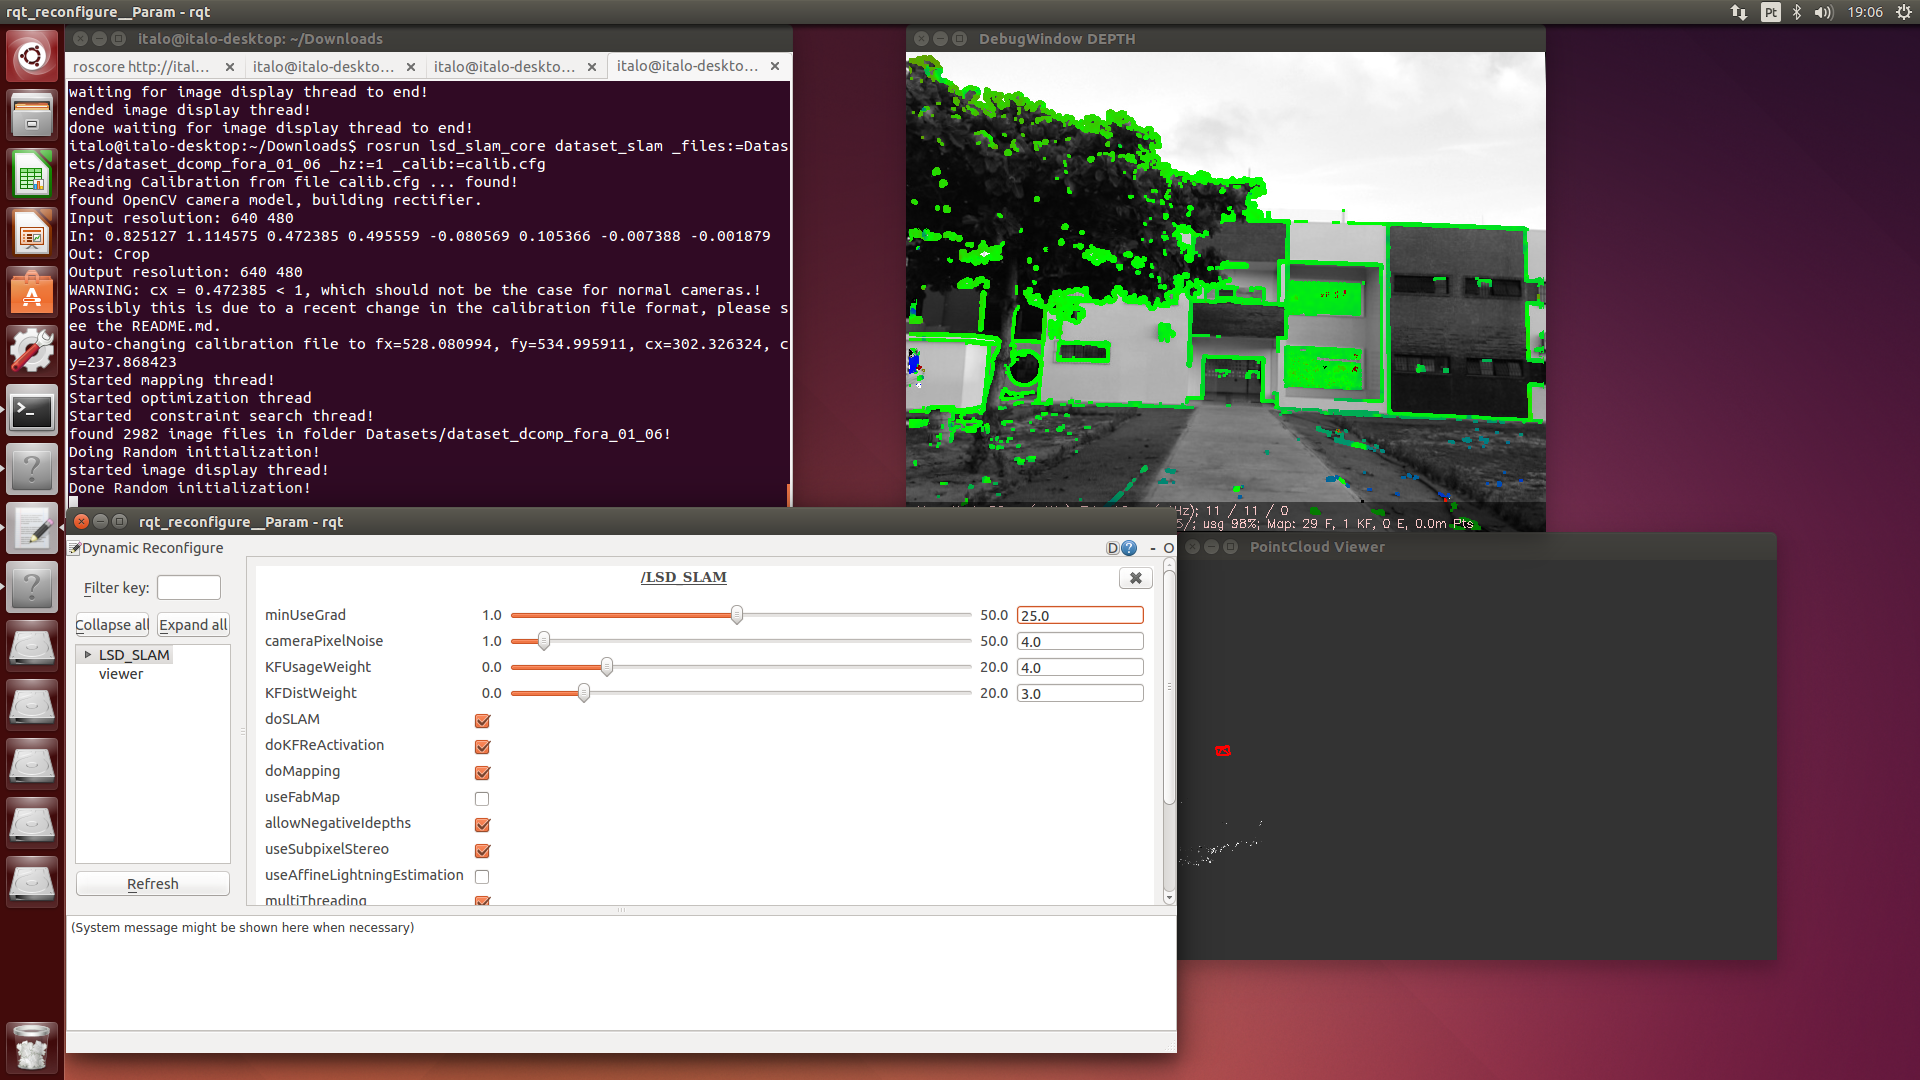
\includegraphics[width= \textwidth]{Imagens/figura3-32.png}
	\caption{\textit{minUseGrad} em 25.0}
	\label{fig3:30}
\end{figure}

Pelos exemplos pode-se perceber que usar o \textit{minUseGrad} no seu valor padrão de 5.0 acrescenta muito ruído devido à grama, além da própria grama ser uma textura que pode ser facilmente confundida gerando erros de relocalização mais à frente na execução. Ao diminuir o parâmetro, a continuidade do gradiente precisa ser mais uniforme para poder ser aceito pelo algoritmo. Não há heurística para a escolha desse valor e ele deve ser testado para cada ambiente. Também vale frisar que aumentar demais esse valor pode cortar alguns gradientes perfeitamente utilizáveis mas que são menos uniformes como por exemplo a passarela até o prédio na imagem.

\subsubsection{\textit{KFUsageWeight e KFDistanceWeight}}


Esses parâmetros influenciam na frequência em que novos \textit{keyframes} são obtidos. O \textit{KFUsageWeight} é em razão da quantidade de quadros usados para refinar, de forma que um número maior faz com que o algoritmo capture novos \textit{keyframes} diminuindo a quantidade de refinamento em cada um consequentemente, como no exemplo a seguir:

\begin{figure}[H]
	\centering
		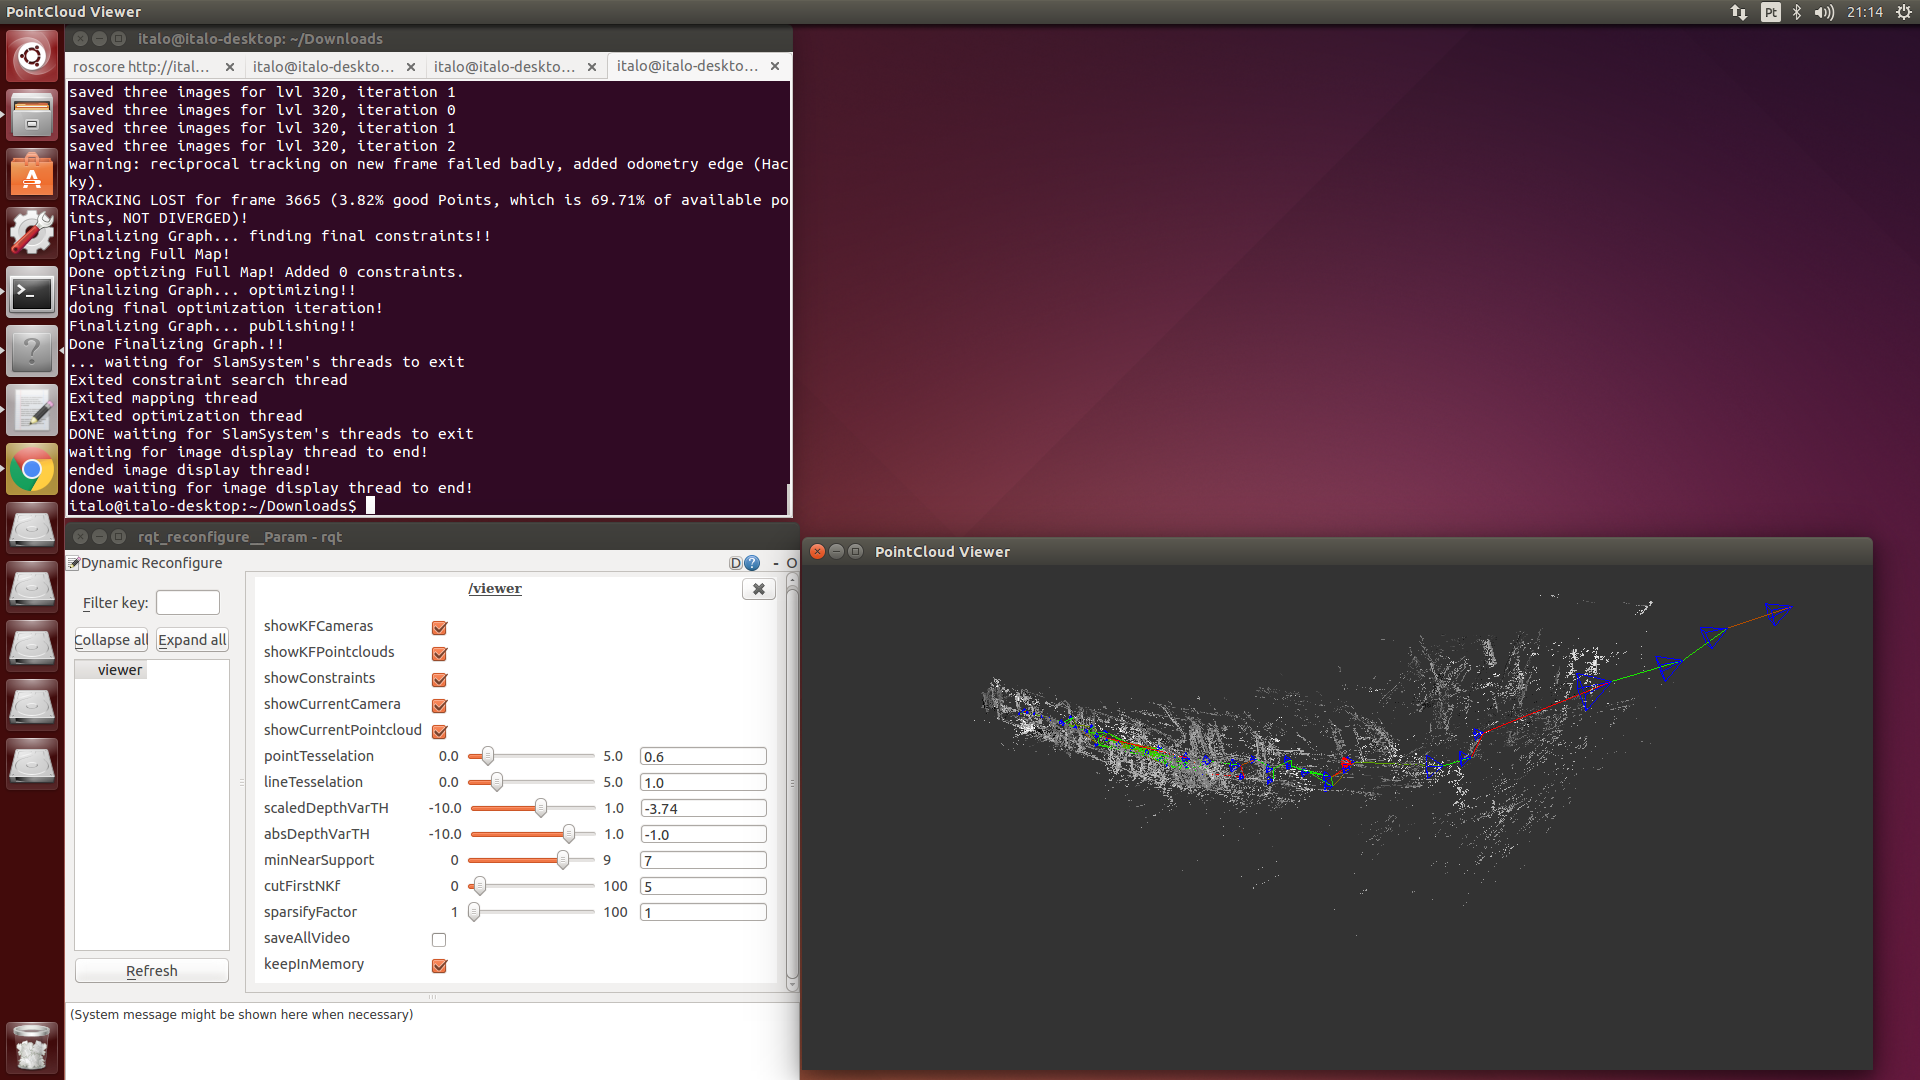
\includegraphics[width= \textwidth]{Imagens/figura3-33.png}
	\caption{\textit{PointCloud} e \textit{keyframes} do corredor do 1º andar do DCOMP usando o \textit{KFUsageWeight} padrão de 4.0 e \textit{KFDistWeight} padrão de 3.0}
	\label{fig3:31}
\end{figure}

\begin{figure}[H]
	\centering
		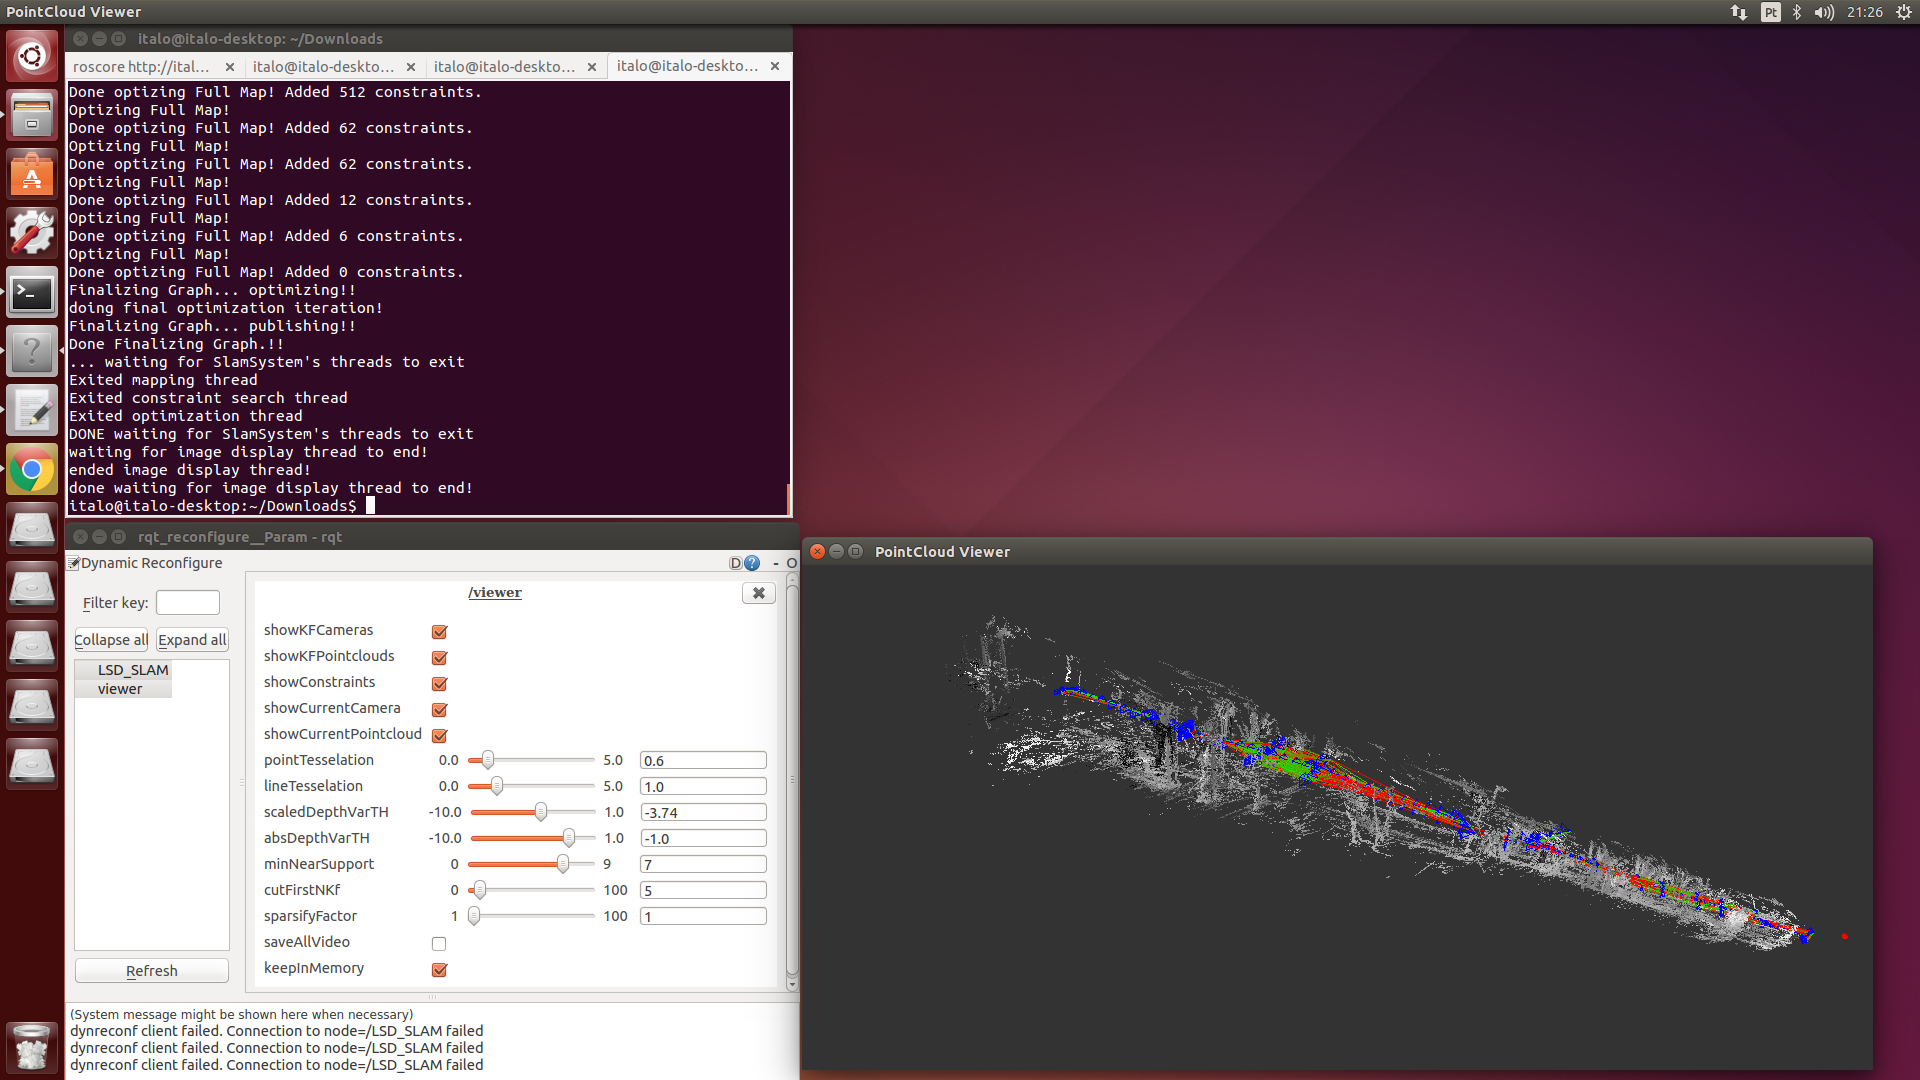
\includegraphics[width= \textwidth]{Imagens/figura3-34.png}
	\caption{\textit{PointCloud} e \textit{keyframes} do corredor do 1º andar do DCOMP usando o \textit{KFUsageWeight} máximo de 20.0 \#1}
	\label{fig3:32}
\end{figure}

\begin{figure}[H]
	\centering
		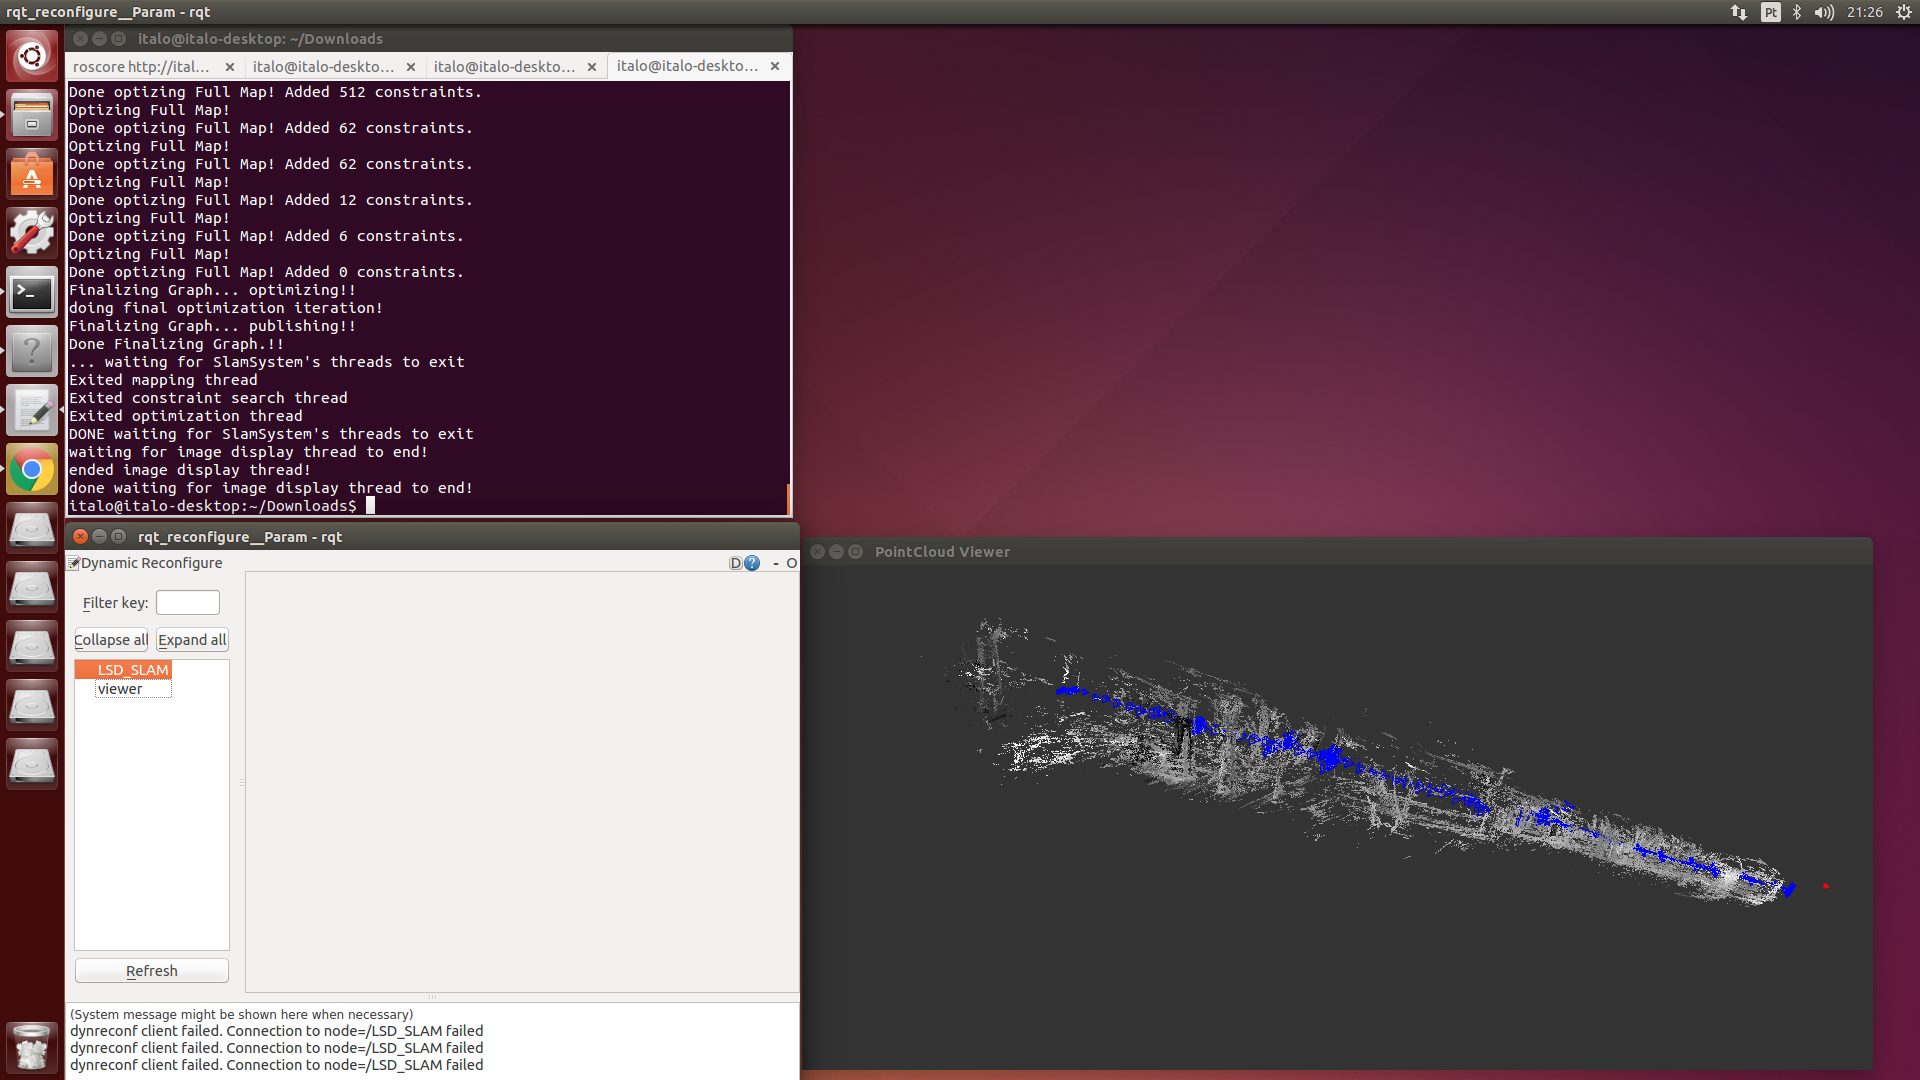
\includegraphics[width= \textwidth]{Imagens/figura3-35}
	\caption{\textit{PointCloud} e \textit{keyframes} do corredor do 1º andar do DCOMP usando o \textit{KFUsageWeight} máximo de 20.0 \#2}
	\label{fig3:33}
\end{figure}


\begin{figure}[H]
	\centering
		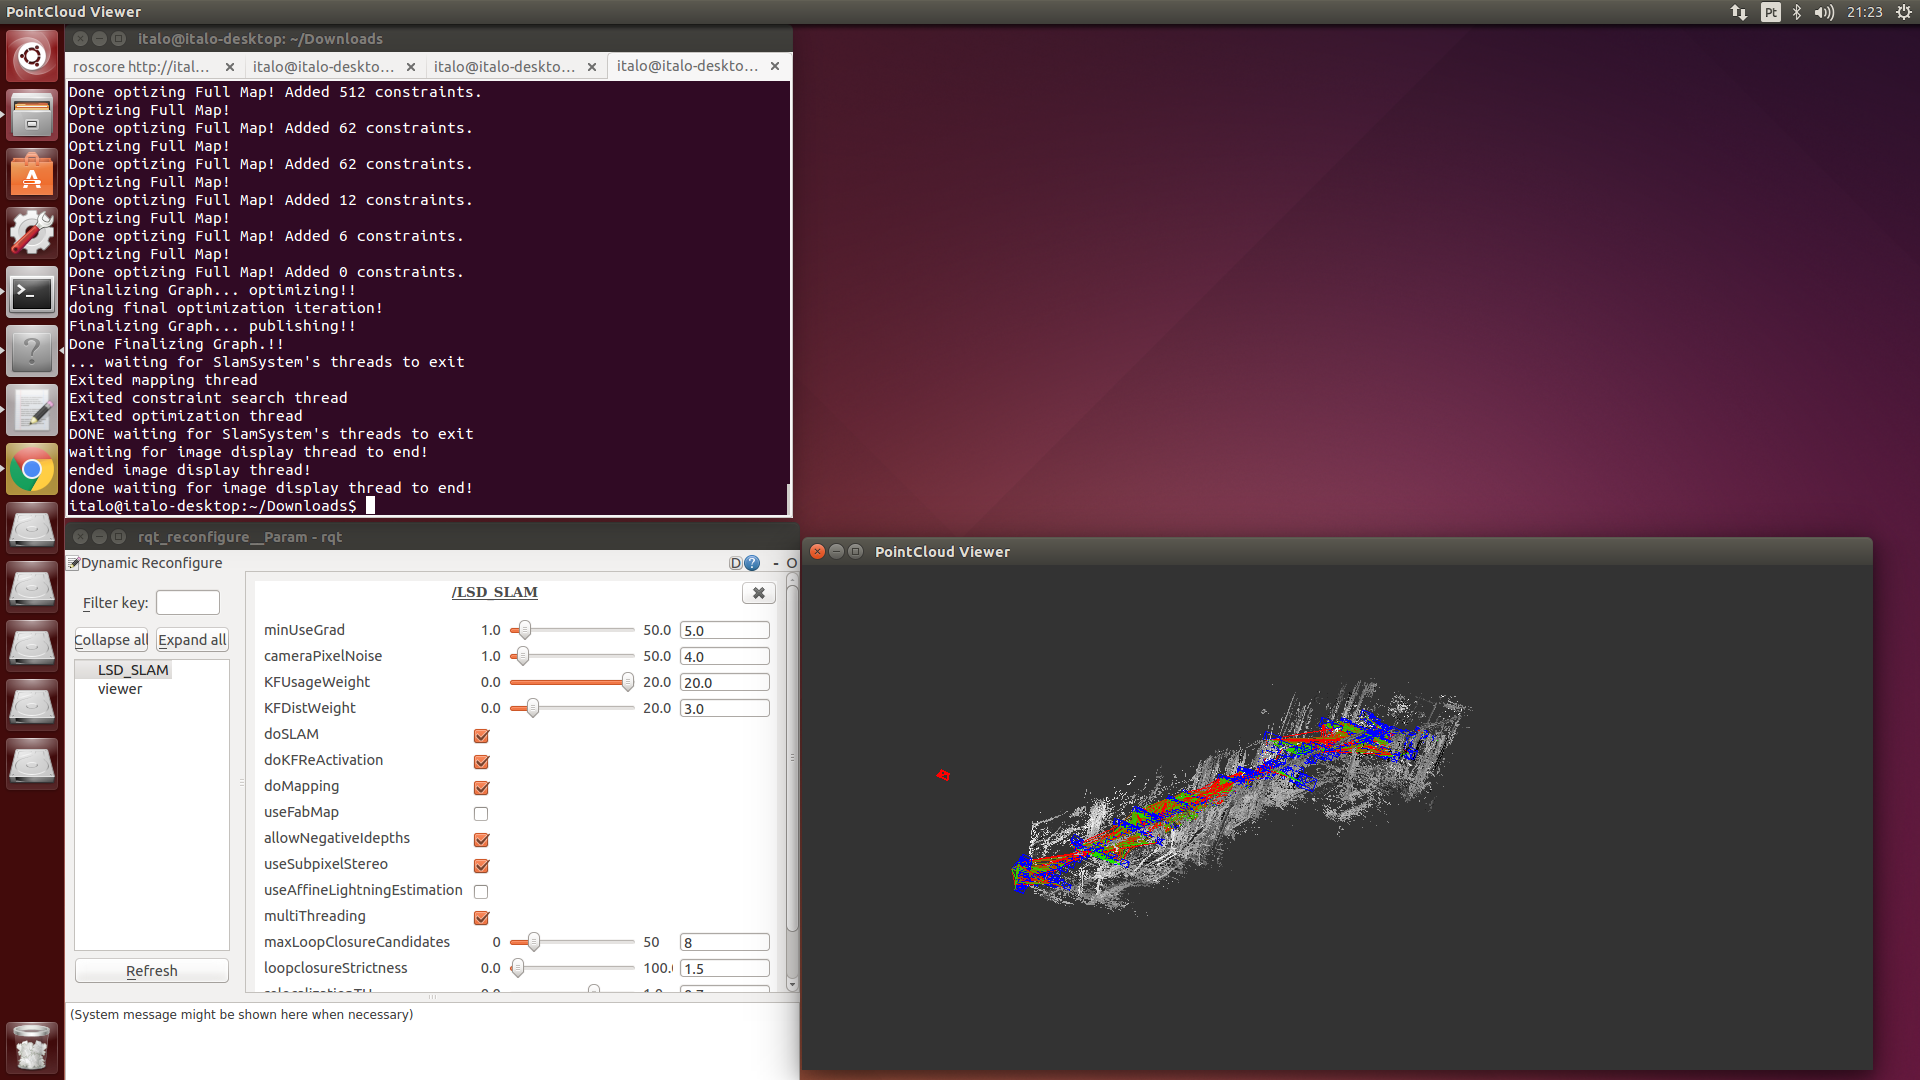
\includegraphics[width= \textwidth]{Imagens/figura3-36.png}
	\caption{\textit{PointCloud} e \textit{keyframes} do corredor do 1º andar do DCOMP usando o \textit{KFUsageWeight} máximo de 20.0 \#3}
	\label{fig3:34}
\end{figure}


\begin{figure}[H]
	\centering
		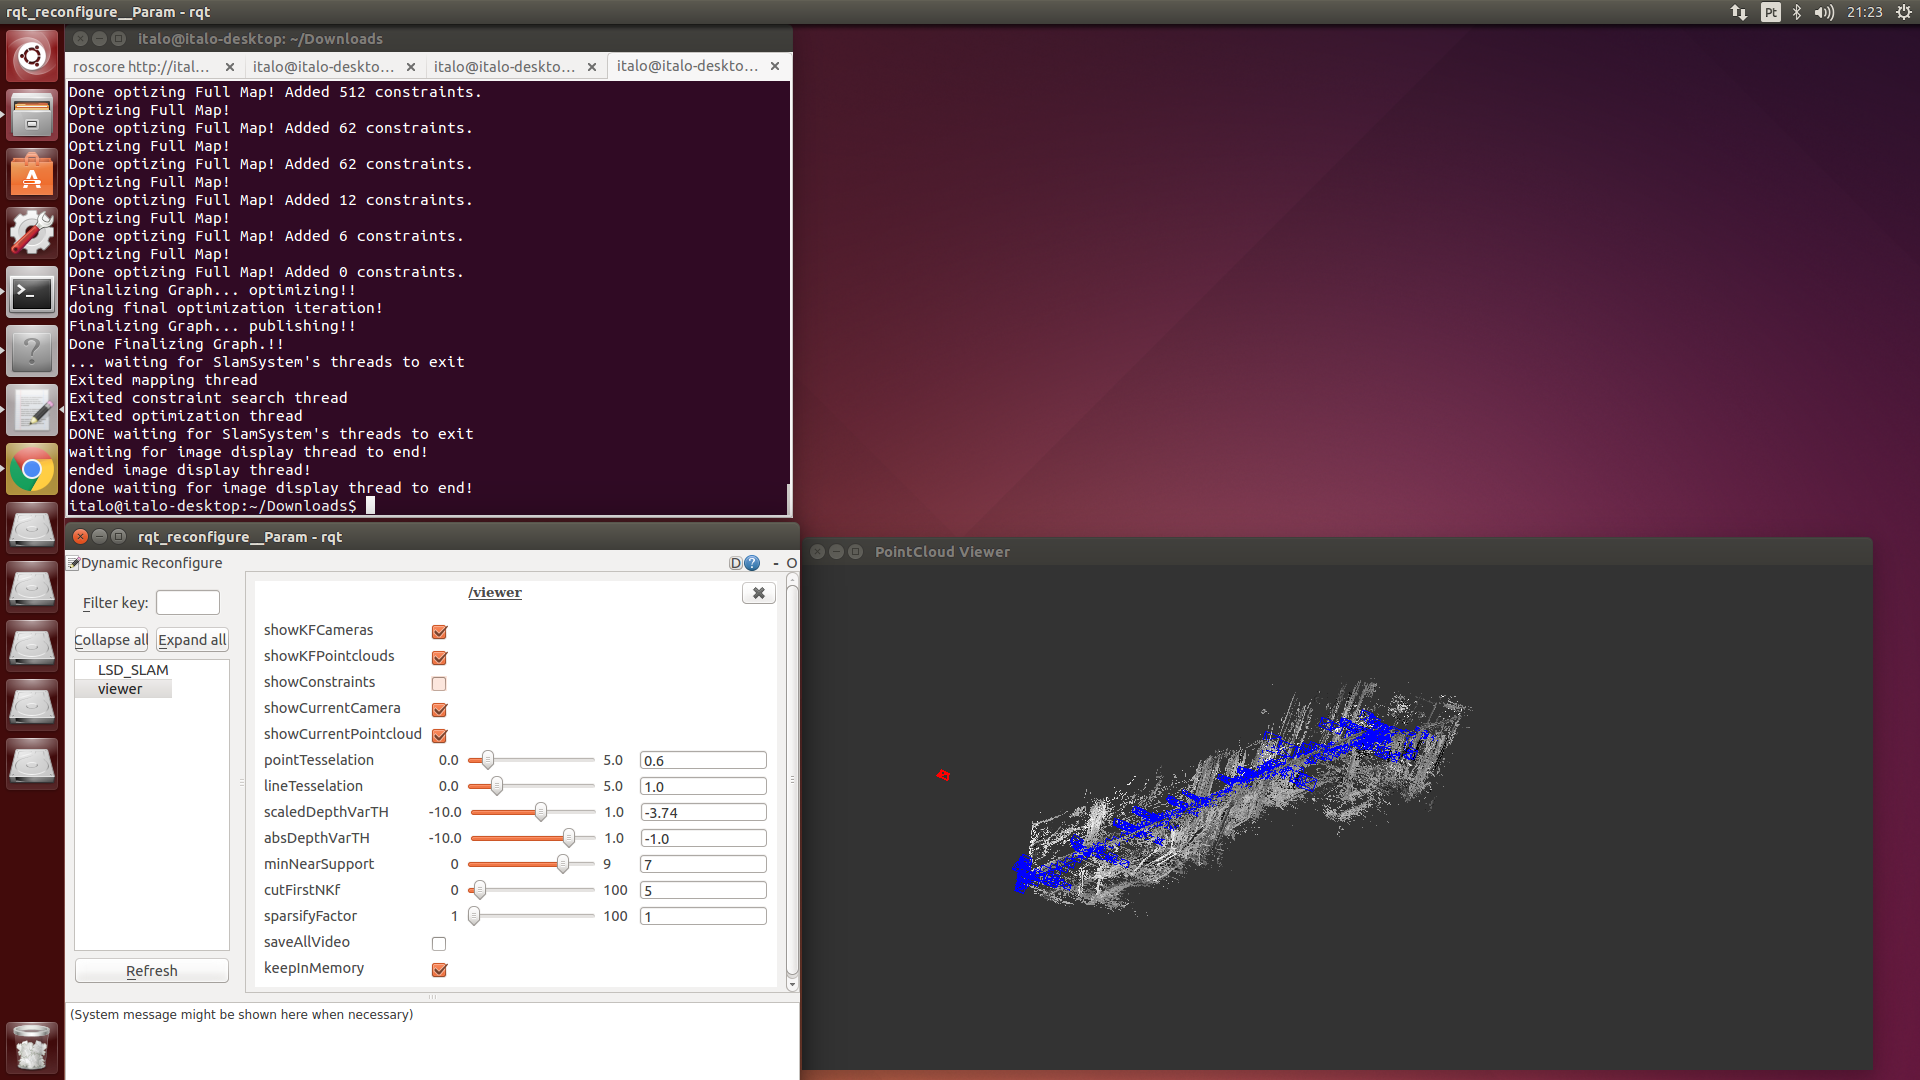
\includegraphics[width= \textwidth]{Imagens/figura3-37.png}
	\caption{\textit{PointCloud} e \textit{keyframes} do corredor do 1º andar do DCOMP usando o \textit{KFUsageWeight} máximo de 20.0 \#4}
	\label{fig3:35}
\end{figure}


Nas janelas do \textit{PointCloud}, as linhas verdes e vermelhas representam \textit{constraints} entre \textit{keyframes} e as pirâmides azuis são \textit{keyframes} e a posição da câmera em relação ao modelo total. Percebe-se que o valor padrão não reproduziu um resultado tão bom quanto o valor máximo, e também pode-se ver que há muito mais \textit{constraints} e \textit{keyframes} nas imagem com o valor máximo. Mas apesar de se ter obtido um resultado melhor dessa forma, há uma carga muito maior de processamento do que pelo valor padrão, fazendo o computador demorar muito mais para executar essa operação devido a quantidade maior de \textit{keyframes} que o algoritmo tem que rastrear e interligar, a ponto dela não ser bem aplicada no \texttt{live\_slam}, e nem em computadores mais lentos/com menor capacidade de processamento. Da mesma forma o \textit{KFDistWeight} também modifica a quantidade de \textit{keyframes}, mas ao contrário do \textit{KFUsageWeight}, ele faz a partir da distância, ou seja, caso o \textit{dataset} possua vários quadros bem próximos fisicamente um do outro e outros quadros mais afastados poderá haver diminuição de \textit{keyframes} no primeiro caso e o aumento de \textit{keyframes} no segundo caso. Isso faz com que o refinamento dos \textit{keyframes} seja mais dependente do \textit{dataset} fazendo com que seja necessário um cuidado maior na hora de movimentar a câmera para não acabar coletando uma quantidade insuficiente de quadros naquela localização. Segue abaixo o mesmo \textit{dataset} usado acima só que com o valor máximo do \textit{KFDistWeight}.

\begin{figure}[H]
	\centering
		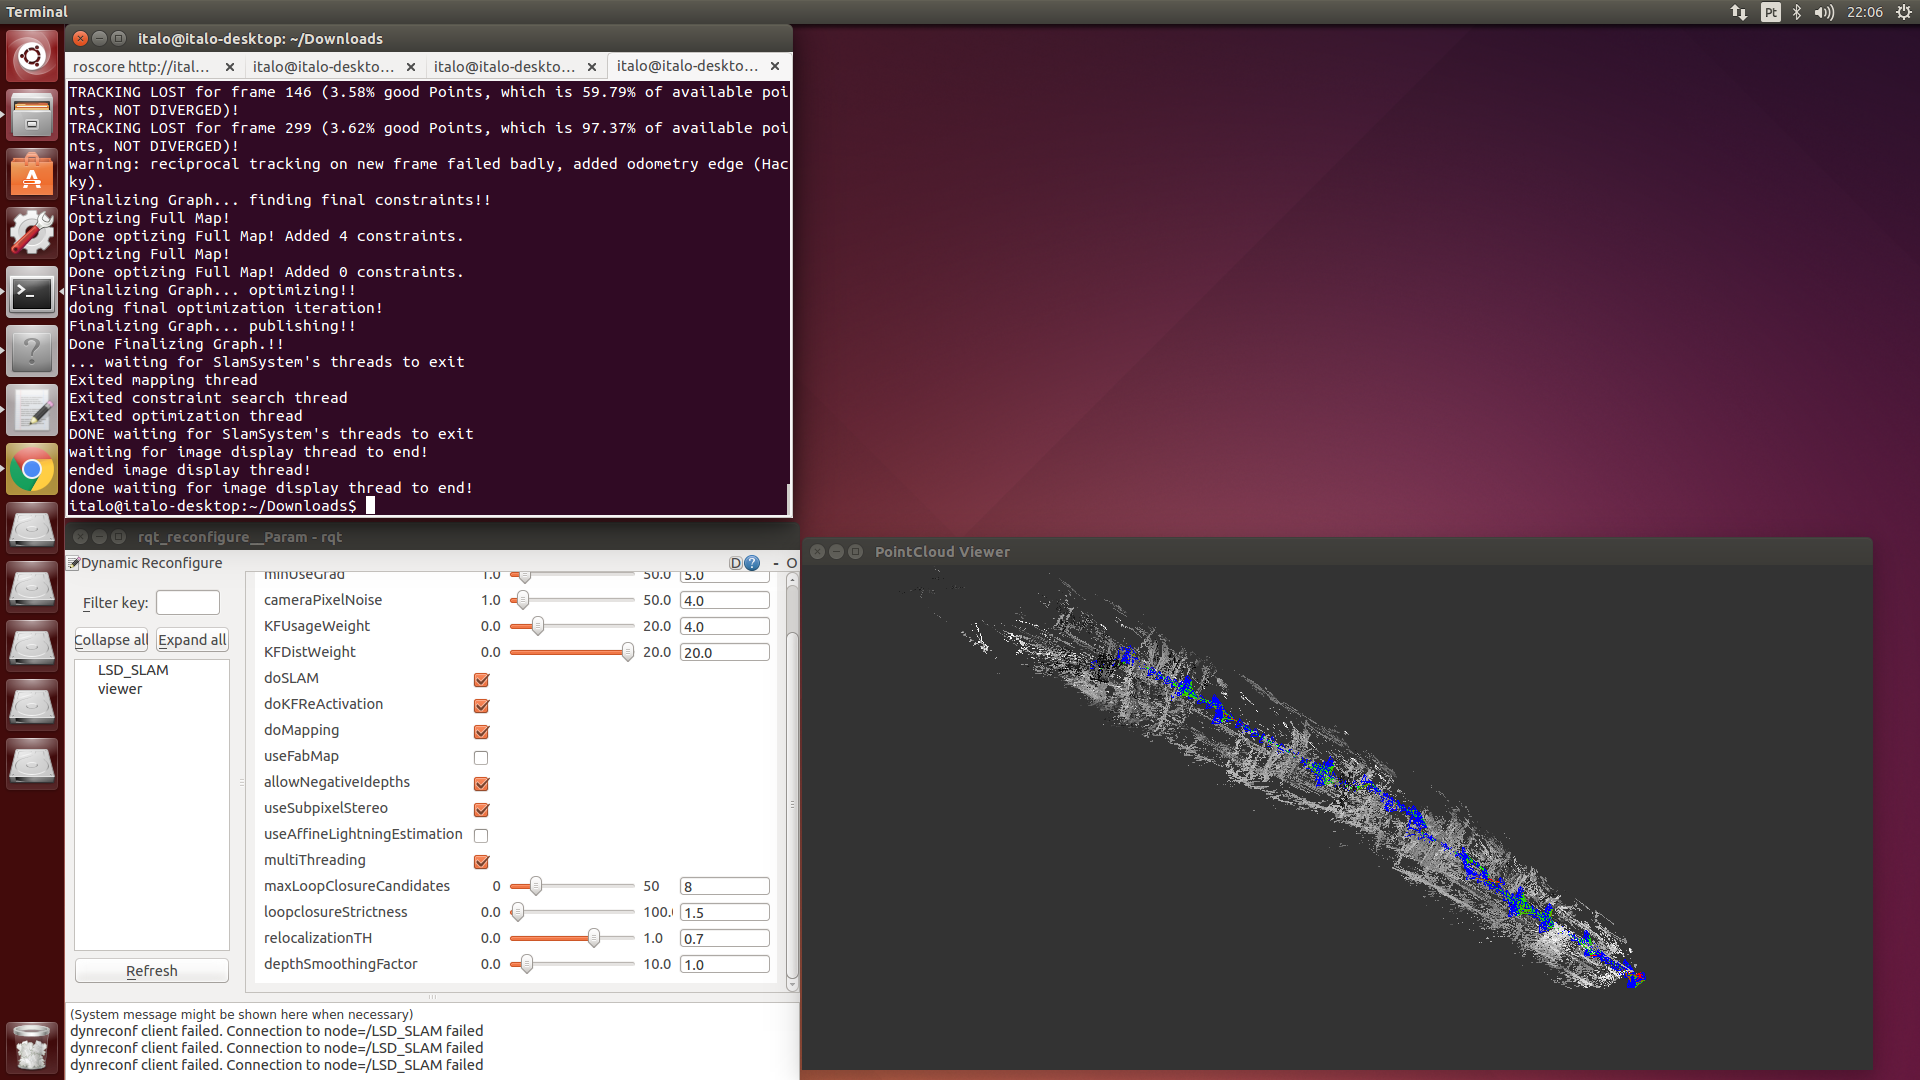
\includegraphics[width= \textwidth]{Imagens/figura3-38.png}
	\caption{\textit{PointCloud} e \textit{keyframes} do corredor do 1º andar do DCOMP usando o \textit{KFDistWeight} máximo de 20.0 \#1}
	\label{fig3:36}
\end{figure}

\begin{figure}[H]
	\centering
		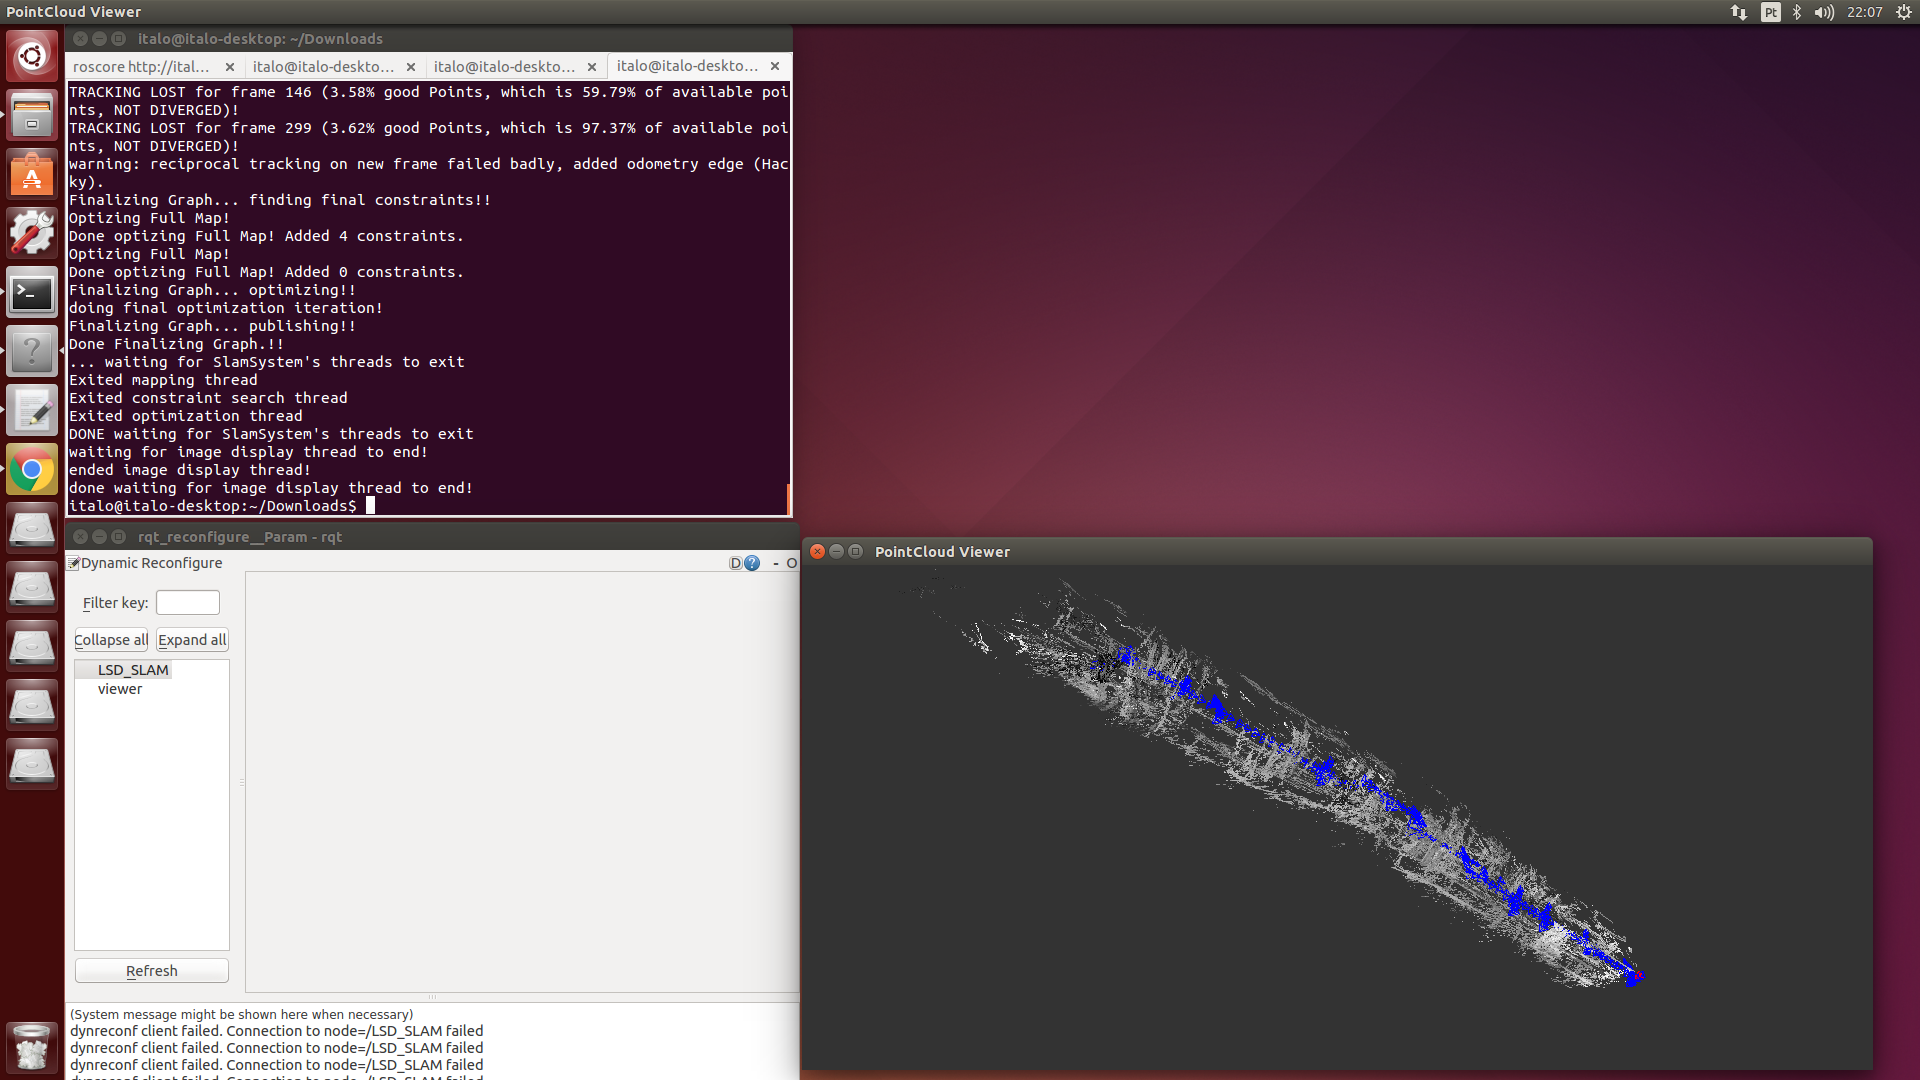
\includegraphics[width= \textwidth]{Imagens/figura3-39.png}
	\caption{\textit{PointCloud} e \textit{keyframes} do corredor do 1º andar do DCOMP usando o \textit{KFDistWeight} máximo de 20.0 \#2}
	\label{fig3:37}
\end{figure}

Como o novo exemplo demonstra, os \textit{keyframes} se comparados aos do valor padrão são mais numerosos, e o resultado geral também foi melhor. O aumento do parâmetro não é tão custoso para máquina como é no \textit{KFUsageWeight}, assim há a possibilidade de usá-lo em computadores com poder de processamento reduzido ou no \texttt{live\_slam}. É importante a experimentação desses parâmetros para se obter o melhor resultado dependendo do \textit{dataset} utilizado e a máquina utilizada. Para concluir essa seção, segue um exemplo do valor máximo de ambos os parâmetros juntos.

\begin{figure}[H]
	\centering
		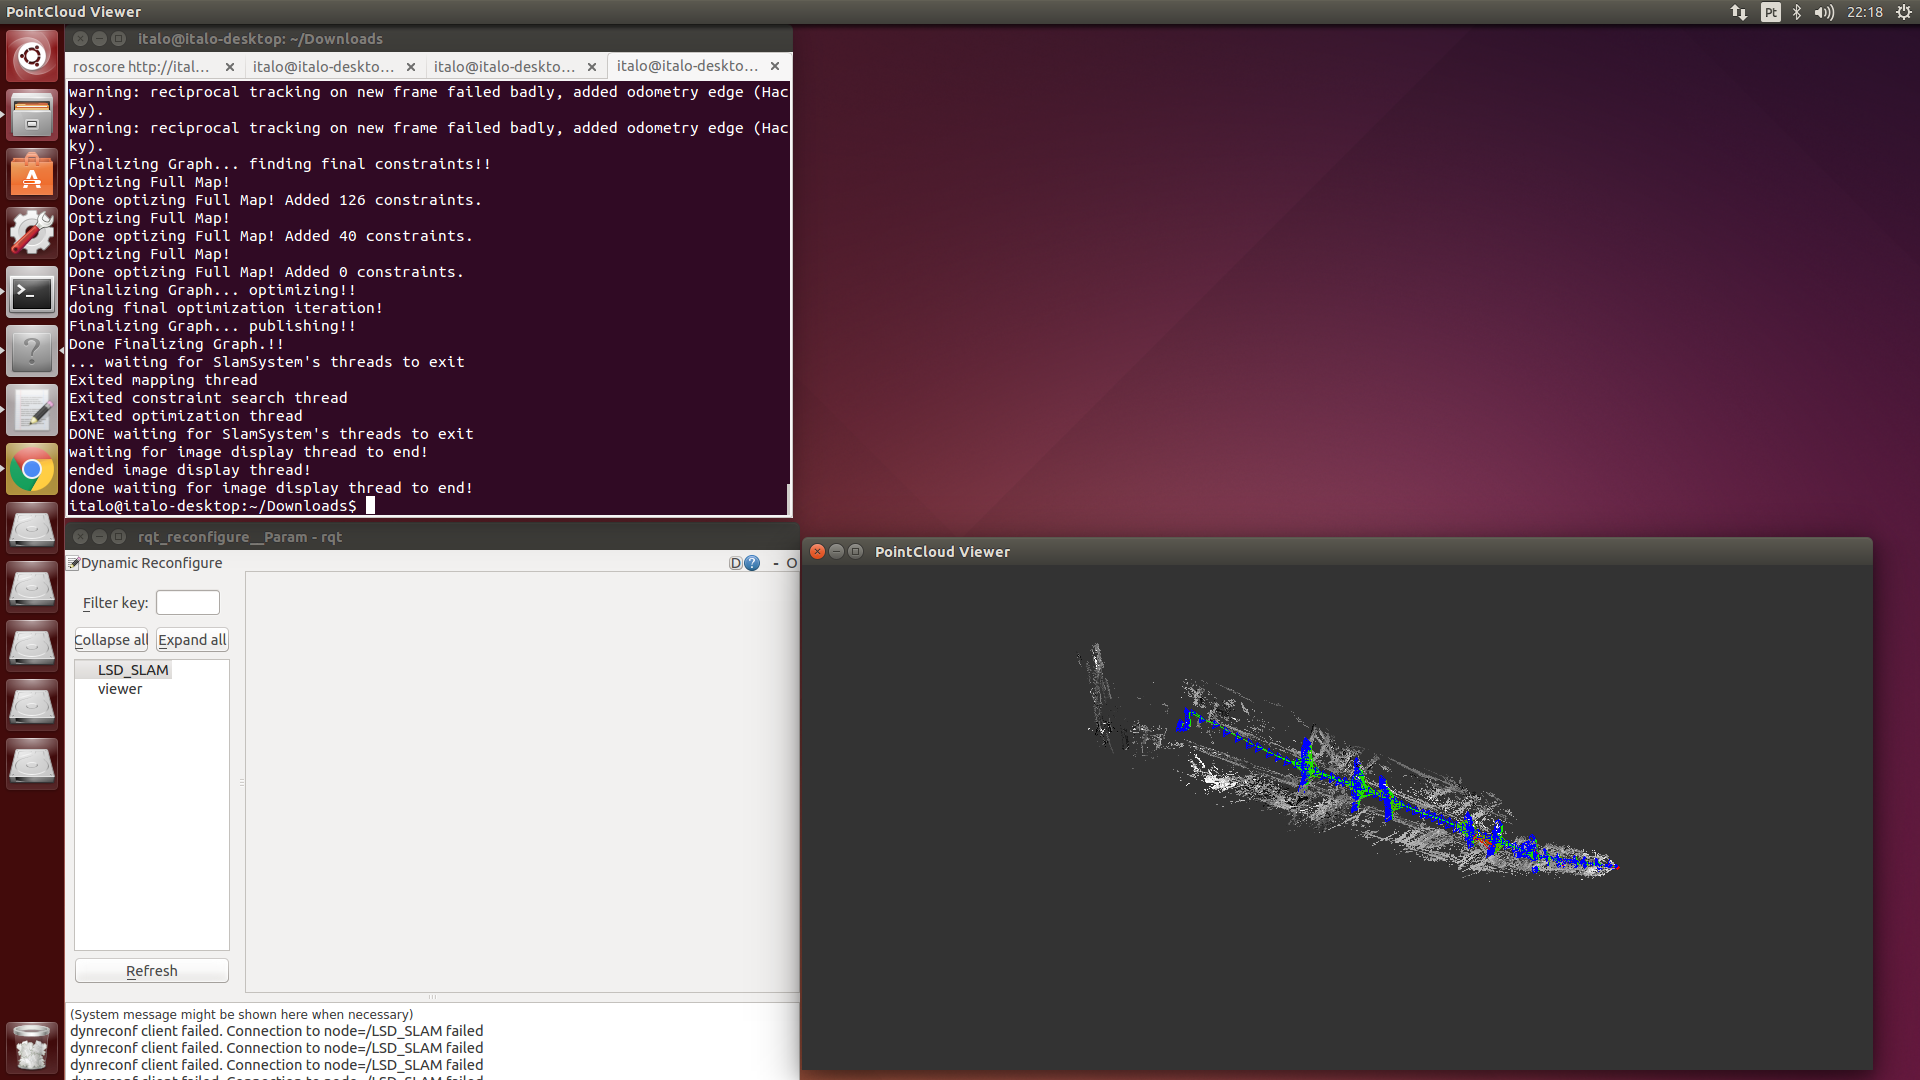
\includegraphics[width= \textwidth]{Imagens/figura3-40.png}
	\caption{\textit{PointCloud} e \textit{keyframes} do corredor do 1º andar do DCOMP usando o \textit{KFUsageWeight} e \textit{KFDistWeight} máximos de 20.0 \#1}
	\label{fig3:38}
\end{figure}

\begin{figure}[H]
	\centering
		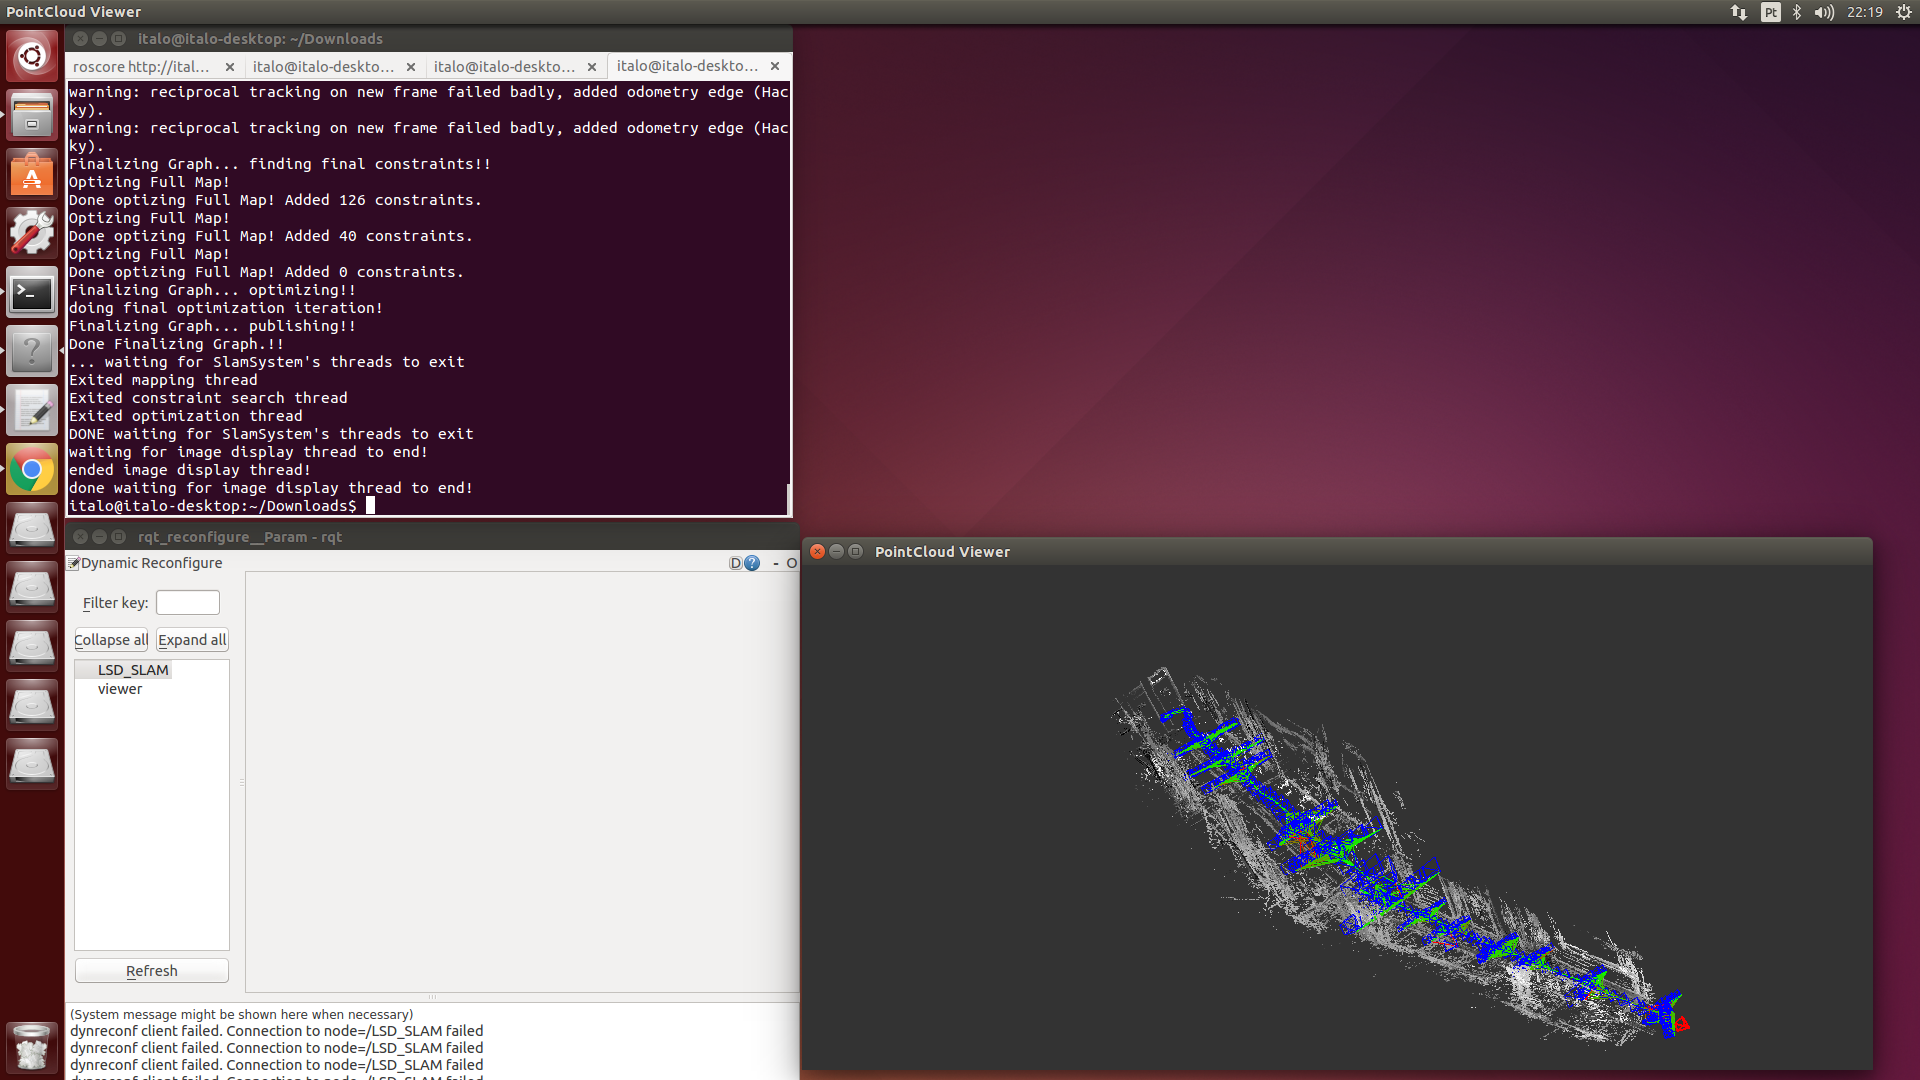
\includegraphics[width= \textwidth]{Imagens/figura3-41.png}
	\caption{\textit{PointCloud} e \textit{keyframes} do corredor do 1º andar do DCOMP usando o \textit{KFUsageWeight} e \textit{KFDistWeight} máximos de 20.0 \#2}
	\label{fig3:39}
\end{figure}
\chapter{Resultados}

Neste capítulo serão apresentados os resultados preliminares, provenientes dos testes realizados bem como refinamento da ferramenta e seus parâmetros. A seção 4.1 apresentará os resultados obtidos com o \textit{PhotoGuide}; na seção 4.2 os resultados preliminares com o \textit{LSD-SLAM} serão mostrados. A seção 4.3 trará os problemas encontrados.

\section{Resultados com o \textit{PhotoGuide}}

Primeiramente o aplicativo operou sem usar nenhuma das três formas de filtragem descritas anteriormente, ocasionando num grande número de falsos casamentos, como apresentam as imagens \ref{fig4:1} e \ref{fig4:2}:

\begin{figure}[H]
	\centering
		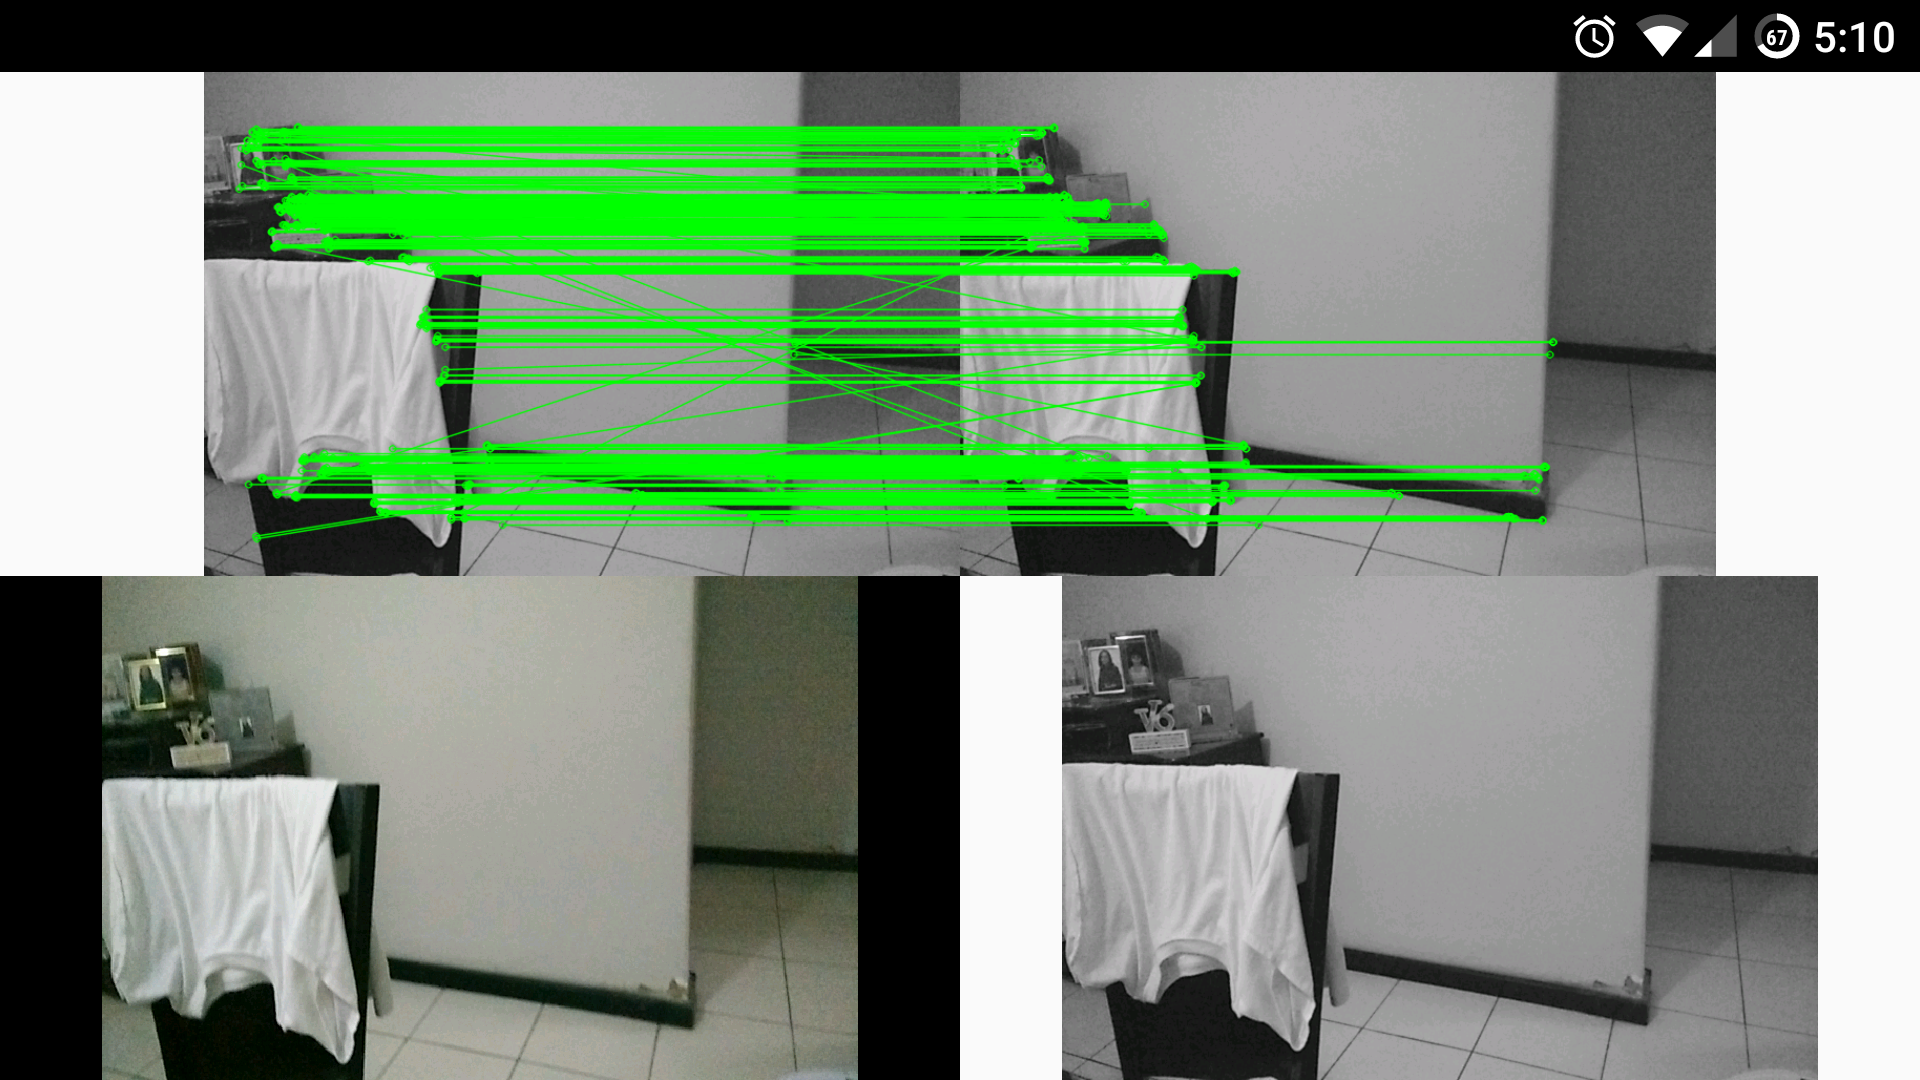
\includegraphics[width= \textwidth]{Imagens/figura4-1.png}
	\caption{Exemplo de execução do \textit{PhotoGuide} sem nenhuma filtragem de casamentos}
	\label{fig4:1}
\end{figure}

\begin{figure}[H]
	\centering
		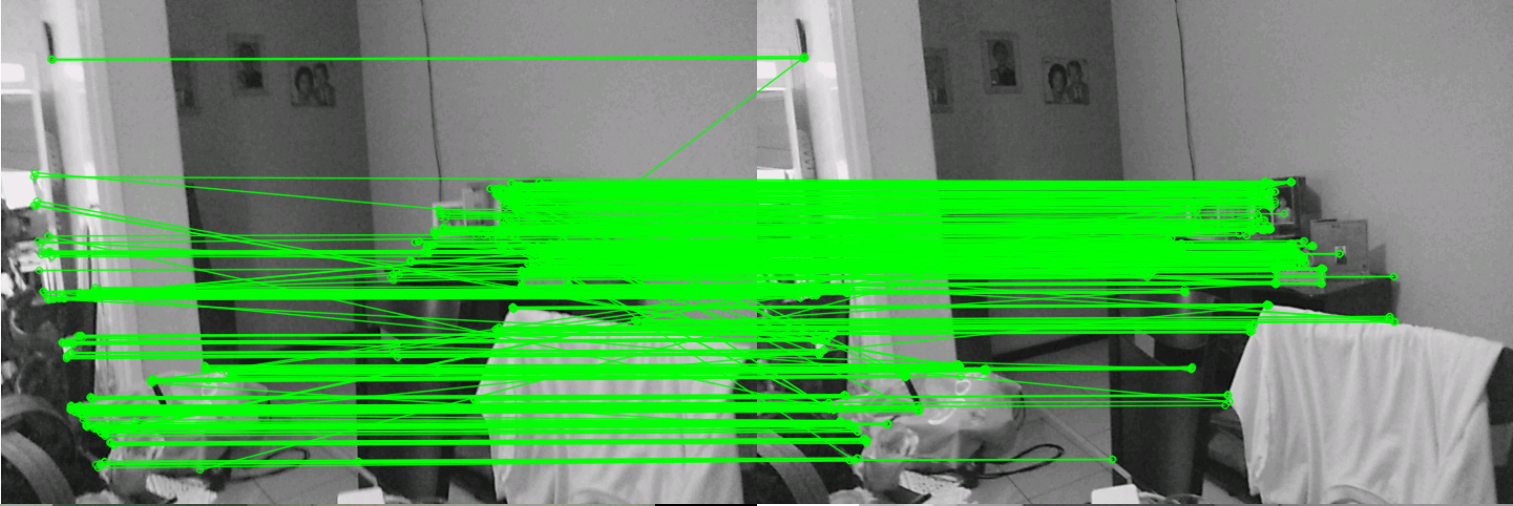
\includegraphics[width= \textwidth]{Imagens/figura4-2.png}
	\caption{Segundo exemplo de execução do \textit{PhotoGuide} sem nenhuma filtragem de casamentos}
	\label{fig4:2}
\end{figure}

Essa situação é pior quando o ambiente possui partes em vidro, como mesas ou janelas, dificultando ainda mais a casamento de pontos, como mostra a Figura \ref{fig4:3}

\begin{figure}[H]
	\centering
		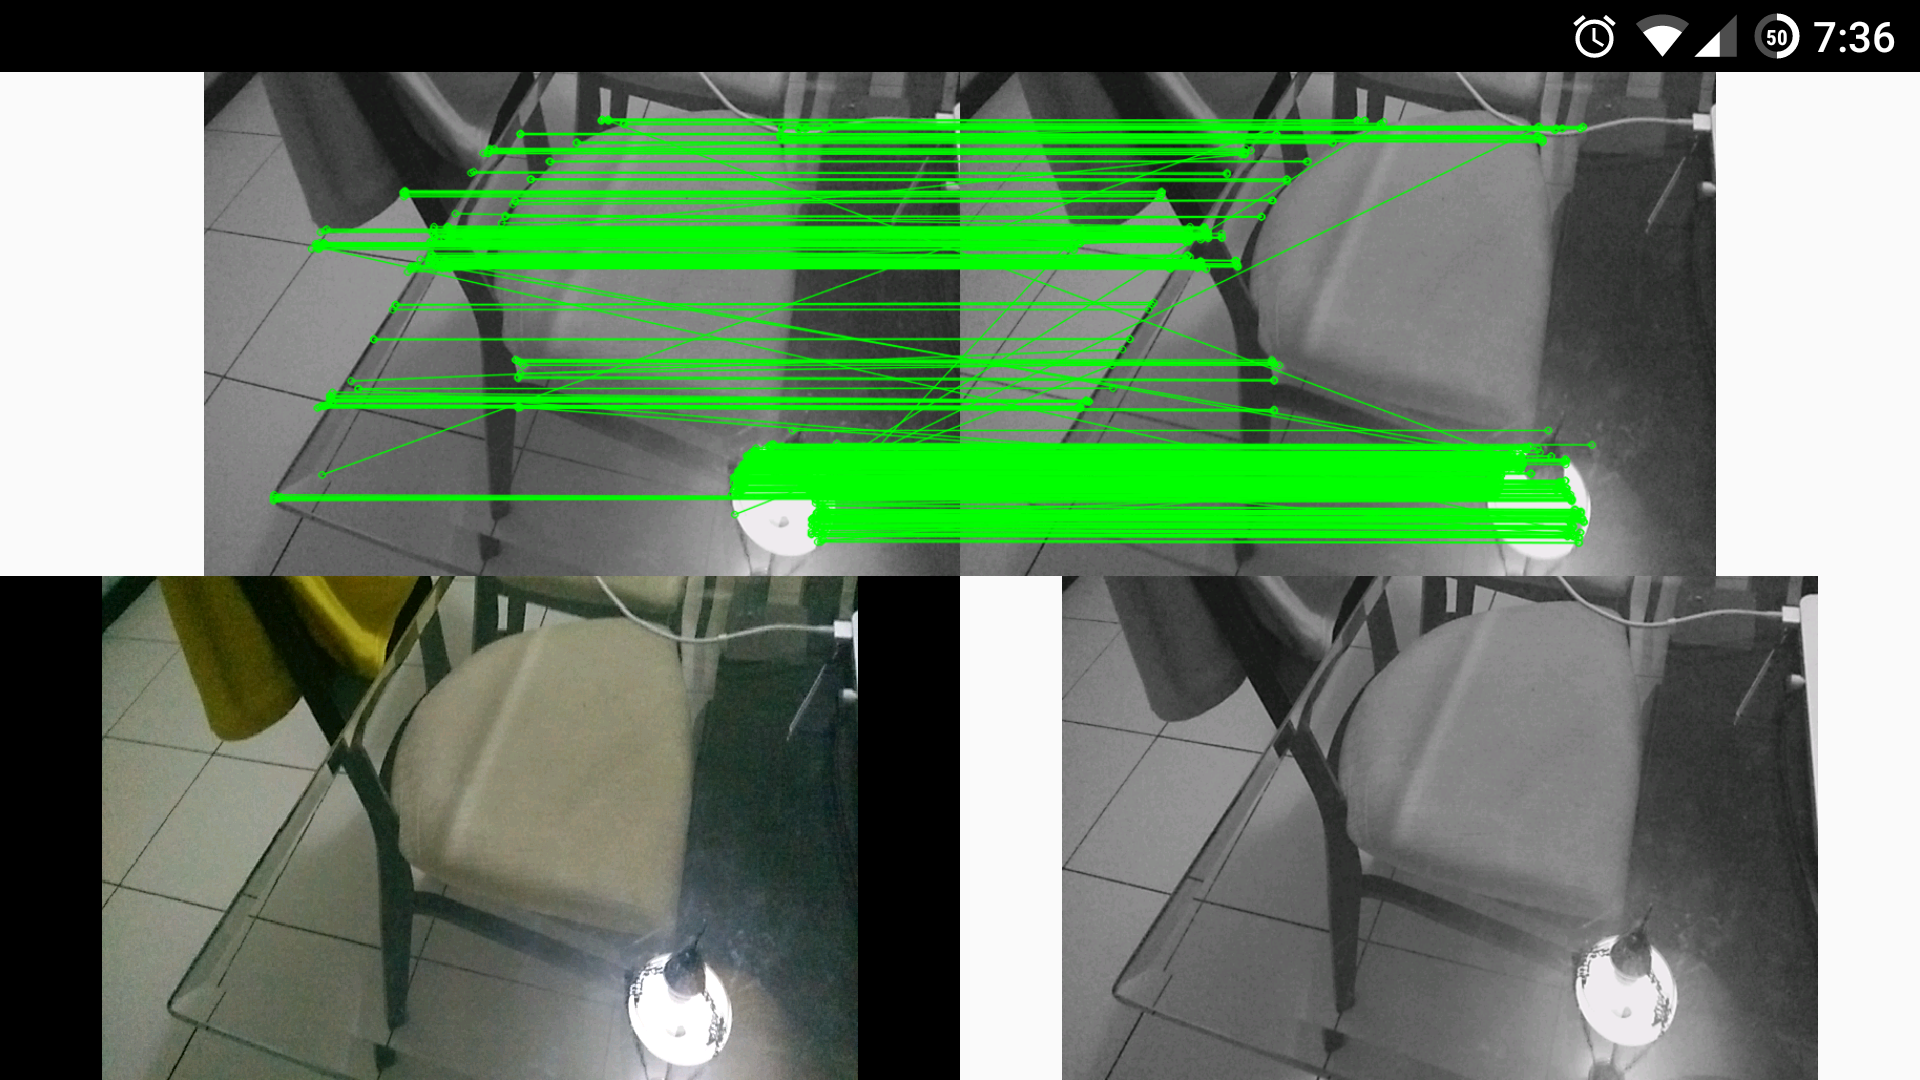
\includegraphics[width= \textwidth]{Imagens/figura4-3.png}
	\caption{Exemplo de execução do \textit{PhotoGuide} sem nenhuma filtragem de casamentos e com peças em vidro, dificultando os casamentos}
	\label{fig4:3}
\end{figure}

Ao se adicionar os métodos de filtragem explicados na seção 3.1, é possível eliminar diversos casamentos errôneos, como na Figura \ref{fig4:4}:

\begin{figure}[H]
	\centering
		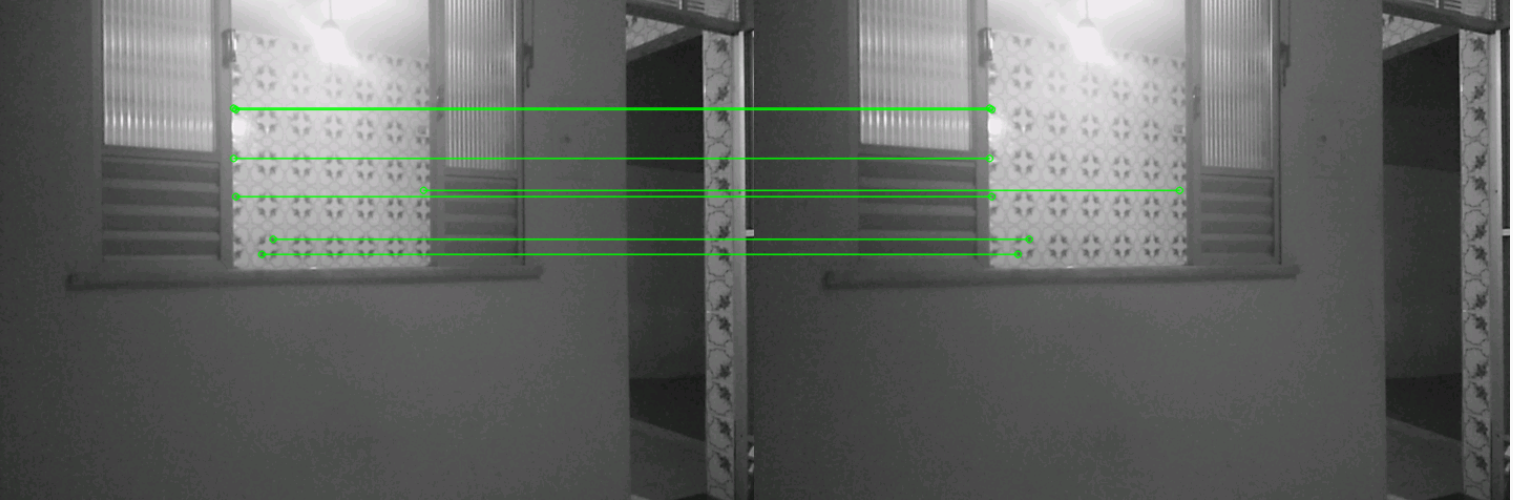
\includegraphics[width= \textwidth]{Imagens/figura3-2E4-4.png}
	\caption{Exemplo da filtragem de casamentos}
	\label{fig4:4}
\end{figure}

Infelizmente, dependendo do ambiente, o número de casamentos pode ser muito pequeno para se tornar significativo para a reconstrução 3D. Foram realizados testes diminuindo a sensibilidade com qual os casamentos eram filtrados, ou a não execução de alguma filtragem, mas ainda eram encontrados falso positivos, sendo necessário todos os métodos de filtragem. 
	Tendo em vista os problemas com o desempenho no aparelho utilizado, bem como problemas com o algoritmo, a continuação do trabalho se deu com a ferramenta \textit{LSD-SLAM}, e a funcionalidade de calibração e exportação de arquivo de calibração do \textit{PhotoGuide} foi útil para utilizar a calibração de \textit{smartphones} em testes com o \textit{LSD-SLAM}, bem como a possibilidade de trabalhos futuros onde seja desejável a exportação da calibração da câmera ou obter \textit{dataset} usando o \textit{smartphone}.
	
\section{Resultados com o \textit{LSD-SLAM}}

O \textit{LSD-SLAM} possui diversos parâmetros que podem auxiliar na visualização e refinamento de como seus algoritmos funcionam. Os testes foram realizados em um dos laboratórios do DCOMP, mais precisamente, o laboratório de mestrado II, na área externa do prédio e também em um quintal, este último para testar os resultados sob um ambiente com mais texturas e menos homogêneo. As Figuras \ref{fig4:5} a \ref{fig4:15} mostram as \textit{PointClouds} obtidas e fotografias dos ambientes:

\begin{figure}[H]
	\centering
		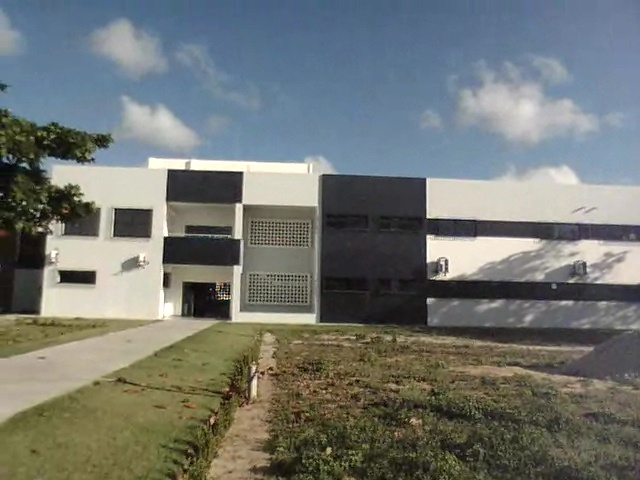
\includegraphics[width= \textwidth]{Imagens/figura4-7.jpg}
	\caption{Fotografia da área externa do DCOMP}
	\label{fig4:7}
\end{figure}

\begin{figure}[H]
	\centering
		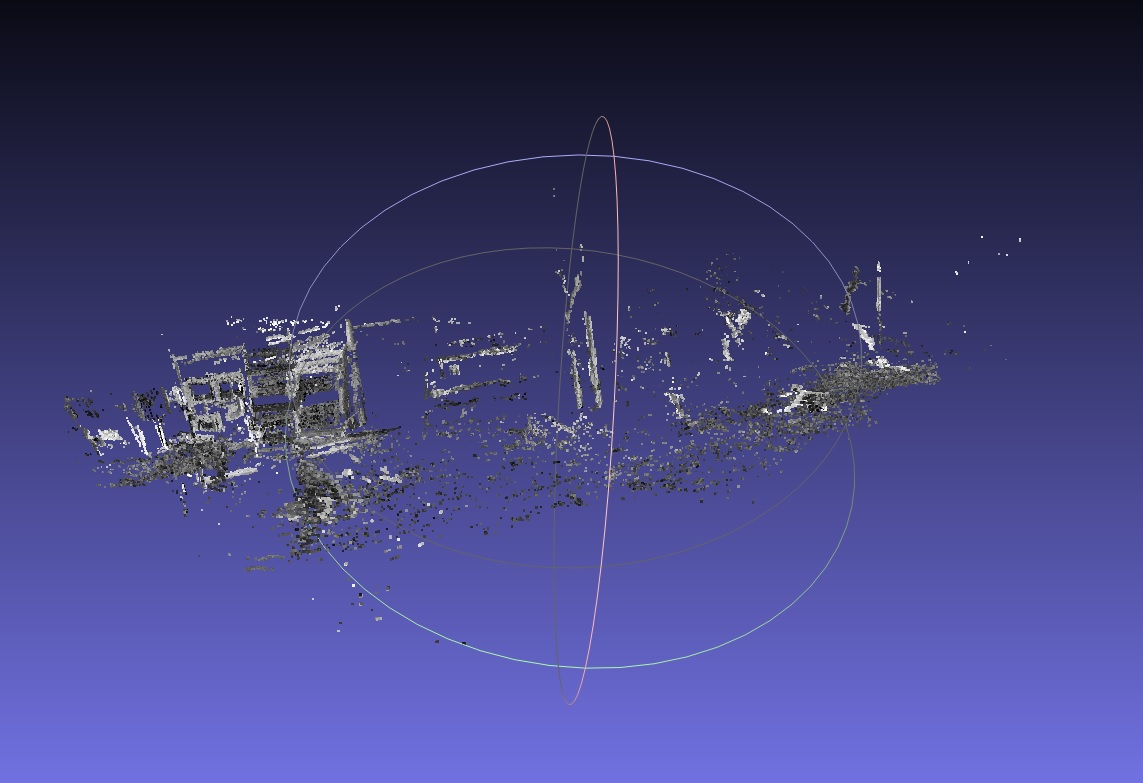
\includegraphics[width= \textwidth]{Imagens/figura4-5.jpg}
	\caption{\textit{Nuvem de pontos} da área externa do DCOMP com a câmera \textit{PSEye®} com 119621 pontos (a)}
	\label{fig4:5}
\end{figure}

\begin{figure}[H]
	\centering
		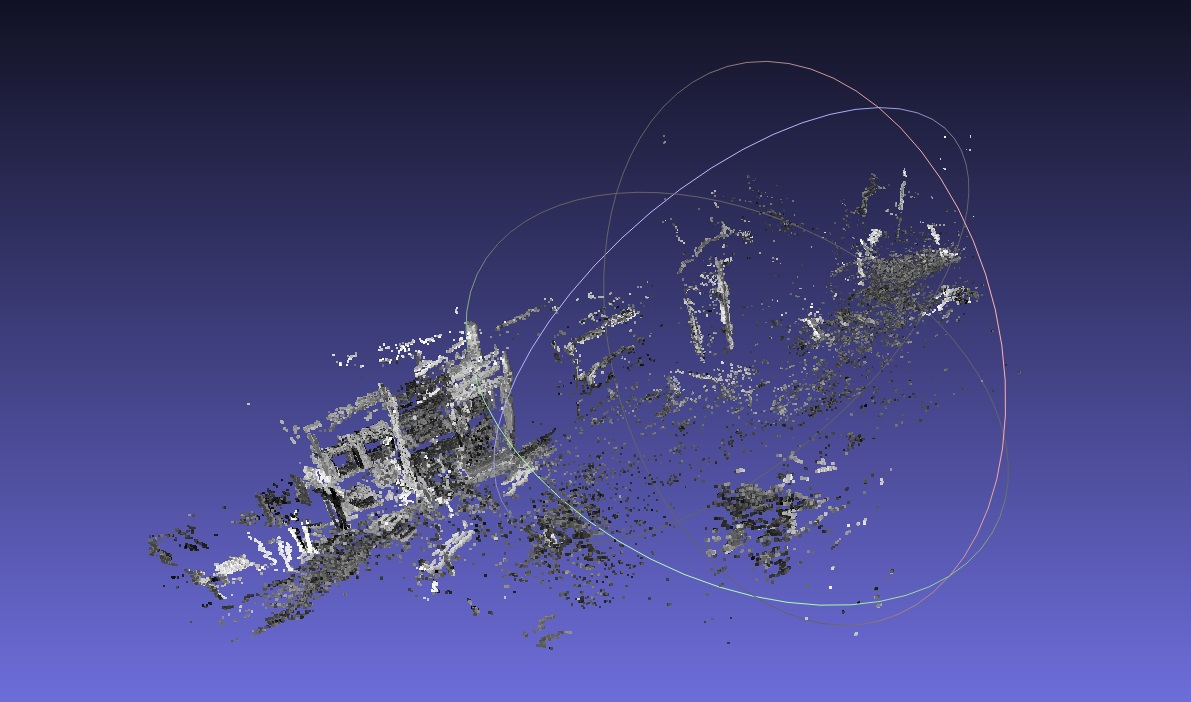
\includegraphics[width= \textwidth]{Imagens/figura4-6.jpg}
	\caption{\textit{Nuvem de pontos} da área externa do DCOMP com a câmera \textit{PSEye®} com 119621 pontos (b)}
	\label{fig4:6}
\end{figure}


\begin{figure}[H]
	\centering
		\includegraphics[width= \textwidth]{Imagens/figura4-8.jpg}
	\caption{Outra \textit{nuvem de pontos} da área externa do DCOMP usando a \textit{PSEye®} com 119621 pontos , sob outro ângulo}
	\label{fig4:8}
\end{figure}

\begin{figure}[H]
	\centering
		\includegraphics[width= \textwidth]{Imagens/figura4-12.jpg}
	\caption{Fotografia do quintal}
	\label{fig4:12}
\end{figure}

\begin{figure}[H]
	\centering
		\includegraphics[width= \textwidth]{Imagens/figura4-10.jpg}
	\caption{\textit{Nuvem de pontos} do quintal de uma casa com 87093 pontos (a)}
	\label{fig4:10}
\end{figure}

\begin{figure}[H]
	\centering
		\includegraphics[width= \textwidth]{Imagens/figura4-11.jpg}
	\caption{\textit{Nuvem de pontos} do quintal de uma casa com 87093 pontos (b)}
	\label{fig4:11}
\end{figure}

\begin{figure}[H]
	\centering
		\includegraphics[width= \textwidth]{Imagens/figura4-15.jpg}
	\caption{Fotografia do laboratório de mestrado II}
	\label{fig4:15}
\end{figure}

\begin{figure}[H]
	\centering
		\includegraphics[width= \textwidth]{Imagens/figura4-13.jpg}
	\caption{\textit{Nuvem de pontos} do laboratório de mestrado II com 168915 pontos (a)}
	\label{fig4:13}
\end{figure}

\begin{figure}[H]
	\centering
		\includegraphics[width= \textwidth]{Imagens/figura4-14.jpg}
	\caption{\textit{Nuvem de pontos} do laboratório de mestrado II com 168915 pontos (b)}
	\label{fig4:14}
\end{figure}

\begin{figure}[H]
	\centering
		\includegraphics[width= \textwidth]{Imagens/dcompMotox.PNG}
	\caption{\textit{Nuvem de pontos} da área externa do DCOMP usando a câmera do \textit{smartphone Motorola® Moto X Play} com 3680087 pontos}
\end{figure}

\begin{figure}[H]
	\centering
		\includegraphics[width= \textwidth]{Imagens/scene00087.jpg}
	\caption{Fotografia do DCOMP usando a câmera do \textit{smartphone Motorola® Moto X Play} com 3680087 pontos}
\end{figure}

\begin{figure}[H]
	\centering
		\includegraphics[width= \textwidth]{Imagens/corredorMotox.PNG}
	\caption{\textit{Nuvem de pontos} do corredor do primeiro andar DCOMP usando a câmera do \textit{smartphone Motorola® Moto X Play} com 5877083 pontos}
\end{figure}

\begin{figure}[H]
	\centering
		\includegraphics[width= \textwidth]{Imagens/corredorMotoxdentro.PNG}
	\caption{\textit{Nuvem de pontos} do corredor do primeiro andar DCOMP usando a câmera do \textit{smartphone Motorola® Moto X Play} por dentro do \textit{PointCloud} com 5877083 pontos}
\end{figure}

As imagens mostram as saídas do algoritmo em diferentes ambientes. Percebe-se que apesar de haver partes incompletas, os mapas oferecem uma informação correta se usados de maneira adequada. Em algumas dessas imagens percebe-se que a definição de profundidade foi insatisfatória devido ao meio em que foram capturados esses \textit{datasets}, no entanto satisfatória para o intuito original de modelagem 3D proposto na introdução.

\section{Problemas}

Alguns problemas encontrados na gravação do \textit{dataset} foram relacionados à luminosidade. Ela afeta fortemente os quadros capturados fazendo com que as imagens tiradas pela câmera sofram problemas de exposição tornando-os inválidos para processamento. Isso se torna mais evidente em ambientes externos sob forte luminosidade ou ambientes internos com pouca luz. O fato que o algoritmo converte todas as imagens usadas também causa problemas no reconhecimento de gradientes caso duas cores tenham a mesma tonalidade. 

A escolha do equipamento também influencia muito, já que inicialmente foi utilizada uma \textit{webcam} da marca \textit{Logitech®} e frequentemente vários quadros eram encontrados distorcidos, pixelados. Ainda sobre o equipamento, foi notado que a falta de foco também prejudica a reconstrução, dado que o algoritmo não consegue realizar casamentos confiáveis onde um dos quadros está embaçado. As Figuras \ref{fig4:16}, \ref{fig4:17} e \ref{fig4:18}  exemplificam alguns casos onde esses problemas ocorreram. Também houve dificuldade em interligar  \textit{datasets} diferentes para tentar criar uma reconstrução mais completa pois os erros nas transições entre ambientes, como por exemplo de um corredor para uma escada ou de um corredor para outro corredor só são descobertos após o processo de extrair cada quadro do vídeo e rodar o \textit{LSD-SLAM}, fazendo com que seja necessário uma re-captura do \text{dataset}. 

\begin{figure}[H]
	\centering
		\includegraphics[width= \textwidth]{Imagens/figura4-16.jpg}
		\caption{Fotografia do exterior do prédio do DCOMP, sombras causadas pelo por do sol atrapalham no reconhecimento de gradientes, a reflexividade do prédio faz com um dos lados fique da mesma cor que o céu e a exposição faz com que a imagem tenha saturações}
	\label{fig4:16}
\end{figure}

\begin{figure}[H]
	\centering
		\includegraphics[width= \textwidth]{Imagens/figura4-17.jpg}
	\caption{Fotografia do interior do prédio do DCOMP, desfocado}
	\label{fig4:17}
\end{figure}

\begin{figure}[H]
	\centering
		\includegraphics[width= \textwidth]{Imagens/figura4-18.jpg}
	\caption{Fotografia do interior do DCOMP, pouca luminosidade}
	\label{fig4:18}
\end{figure}
\chapter{Conclusão}

\lipsum

% ----------------------------------------------------------
% ELEMENTOS PÓS-TEXTUAIS
% ----------------------------------------------------------
\postextual
\include{glossario}
\include{apendices}
\chapter{Anexo}



\section{Instalação da estação de trabalho}

Este capítulo foi incluído para servir de referência aos leitores que desejarem usar a ferramenta \textit{LSD-SLAM} no futuro. Contém algumas informações que consideramos úteis e soluções para alguns dos problemas encontrados.

Etapas para preparação:

\begin{enumerate}
	\item{Instalação do \textit{Ubuntu}: A instalação do \textit{Ubuntu} deve ser da versão 12 ou 14 obrigatoriamente, a versão usada no trabalho foi a 14.04.}
	\item{Instalação do  \textit{ROS}: O \textit{ROS} vai ser utilizado para a leitura dos quadros da câmera/\textit{dataset} além de ser onde a ferramenta é implementada.\cite{ROS-Tutorial}}
	\item{Instalação do \textit{LSD-SLAM}.\cite{GitHub-LSD-SLAM}}
	\item{Instalação do  \texttt{usb\_cam}: \texttt{usb\_cam} é um \textit{driver} \textit{ROS} para habilitar câmeras \textit{USB} a serem utilizadas como \textit{stream} de dados para o \textit{ROS} e consequentemente o \textit{LSD-SLAM}, se não há intenção de usar câmeras, como quando utilizando um \textit{dataset}, o \textit{driver} \textit{USB} não é necessário.}
	\item{Calibração da câmera: Será detalhada nas próximas seções.}
\end{enumerate}

\section{Calibração da câmera}

Uma calibração da câmera do \textit{OpenCV} pode ser usada na \textit{LSD-SLAM}, no entanto ela vem, na sua instalação, com uma ferramenta de calibração mais intuitiva e confiável por oferecer um retorno ao usuário se as amostras tiradas são o suficiente ou não. Além disso câmeras \textit{USB} não podem ser configuradas usando o \textit{software} \textit{Android} \textit{PhotoGuide}.

\subsection{Imprimindo o padrão tabuleiro de xadrez}

Antes de utilizar a câmera deve-se calibrá-la a fim de eliminar a distorção radial que possa ocorrer ao se capturar quadros da mesma forma que no \textit{OpenCV}.
Primeiramente deve-se imprimir um tabuleiro de xadrez \cite{Setup-CalibrateMonocularCamera}, preferencialmente em uma folha ou cartolina A3 ou A4 e fixado em uma superfície rígida e plana.

Todos esses fatores interferem no reconhecimento do padrão, fazendo com que o resultado da calibração se torne falho. Com o tabuleiro em mãos, tomando cuidado para não cobrir as “casas” do tabuleiro, o desensenvolvedor move-se para um lugar espaçoso de pelo menos 3x3 m, livre de obstruções e bem iluminado.

\subsection{Compilando e construindo a ferramenta de calibração}

Começa-se obtendo as dependências necessárias e compilando o \textit{driver} usando os seguintes comandos respectivamente:

\begin{table}[H]\label{tb:1}
\begin{tabular}{| p{\textwidth}|}
\hline
\texttt{\$ rosdep install camera\_calibration} \\
\texttt{\$ rosmake camera\_calibration} \\ \hline
\end{tabular}
\caption{Comandos para inicializar a instalação do módulo que fará a calibração da câmera}
\end{table}


\subsection{Envio de quadros pela câmera}

Antes de começar a calibração deve-se concluir configuração do pacote usb\_cam e a câmera deve estar conectada e configurada pelo pacote. Para ter certeza que a câmera está de fato enviando seus dados para o \textit{ROS}, usa-se o seguinte comando:

\begin{table}[H]\label{tb:2}
\begin{tabular}{| p{\textwidth}|}
\hline
\texttt{\$ rostopic list}\\
\hline
\end{tabular}
\caption{Comandos para inicializar a instalação do módulo que fará a calibração da câmera}
\end{table}

Esse comando irá listar todos os \textit{topics} que são os nodos ativos no \textit{ROS}. A saída deve conter esses \textit{topics}:

\begin{table}[H]\label{tb:3}
\begin{tabular}{| p{\textwidth}|}
\hline
\texttt{/usb\_cam/camera\_info} \\
\texttt{/usb\_cam/image\_raw}\\
\hline
\end{tabular}
\caption{Resultado com os \textit{topics}}
\end{table}

Caso a saída não apresente erros, a câmera está pronta para ser calibrada.

\subsection{Rodando o nodo de calibração}

Para começar a calibração é necessário carregar os \textit{topics} com as imagens da câmera que será calibrada usando o seguinte comando:

\begin{table}[H]\label{tb:4}
\begin{tabular}{| p{\textwidth}|}
\hline
\texttt{\$ rosrun camera\_calibration cameracalibrator.py --size 9x6 --square 0.108 image:=/usb\_cam/image\_raw camera:=/usb\_cam}\\
\hline
\end{tabular}
\caption{Inicialização do módulo que calibrará a câmera}
\end{table}

Vale frisar a importância de que o parâmetro \texttt{--size} é o tamanho do tabuleiro, no entanto ele conta não as casas e sim as linhas entre as casas:

\begin{figure}[H]
	\centering
		\includegraphics[width= \textwidth]{Imagens/figura3-3E3-12.png}
	\caption{Exemplo de padrão utilizado para a calibração}
	\label{fig3:12}
\end{figure}


Esse padrão por exemplo tem 10x7 casas, no entanto suas linhas são 9x6. Logo o parâmetro \texttt{--size} deve ser 9x6.
O parâmetro \texttt{--square} é o tamanho real do lado das casas do tabuleiro que imprimimos em metros. O comando acima indica que cada casa do tabuleiro possui 0,108 metros ou 10,8 centímetros. É recomendado que o usuário que reproduza estes passos use uma régua para medir o seu tabuleiro.
Após executar o comando, a janela de calibração será aberta, como mostra a figura 3.13:

\begin{figure}[H]
	\centering
		\includegraphics[width= \textwidth]{Imagens/figura3-13.png}
	\caption{Janela de configuração reconhecendo do tabuleiro \cite{Documentacao-CalibrateMonocularCamera}}
	\label{fig3:13}
\end{figure}

\subsection{Movendo o tabuleiro}

Para se obter uma boa calibração é necessário mover o tabuleiro pelo quadro da câmera de modo que:

\begin{itemize}
	\item{O tabuleiro se encontre nas partes esquerda, direita, superior e inferior do campo de vista da câmera.}
	\begin{itemize}
		\item{Barra X - Campo de vista esquerda/direita.}
		\item{Barra Y - Campo de vista topo/baixo.}
		\item{Barra \textit{Size} - Aproximando/Afastando e Rotação da câmera.}
	\end{itemize}
	\item{O tabuleiro preencha todo o campo de vista.}
	\item{O tabuleiro inclinado para a esquerda,direita,topo,baixo (Barra \textit{Skew})}
\end{itemize}

A cada passo segure o tabuleiro até que que apareça na imagem o destaque do padrão.

\begin{figure}[H]
\minipage{0.32\textwidth}
  \caption{Desmonstração de posição para calibração \#1 \cite{Documentacao-CalibrateMonocularCamera}}\label{fig3:14}
  \includegraphics[width=\linewidth]{Imagens/figura3-14.png}
\endminipage\hfill
\minipage{0.32\textwidth}
  \caption{Desmonstração de posição para calibração \#2 \cite{Documentacao-CalibrateMonocularCamera}}\label{fig3:15}
  \includegraphics[width=\linewidth]{Imagens/figura3-15.png}
\endminipage\hfill
\minipage{0.32\textwidth}
  \caption{Desmonstração de posição para calibração \#3 \cite{Documentacao-CalibrateMonocularCamera}}\label{fig3:16}
  \includegraphics[width=\linewidth]{Imagens/figura3-16.png}
\endminipage
\end{figure}

\begin{figure}[H]
\minipage{0.32\textwidth}
  \includegraphics[width=\linewidth]{Imagens/figura3-17.png}
  \caption{Desmonstração de posição para calibração \#4 \cite{Documentacao-CalibrateMonocularCamera}}\label{fig3:17}
\endminipage\hfill
\minipage{0.32\textwidth}
  \includegraphics[width=\linewidth]{Imagens/figura3-18.png}
  \caption{Desmonstração de posição para calibração \#5 \cite{Documentacao-CalibrateMonocularCamera}}\label{fig3:18}
\endminipage\hfill
\minipage{0.32\textwidth}
  \includegraphics[width=\linewidth]{Imagens/figura3-19.png}
  \caption{Desmonstração de posição para calibração \#6 \cite{Documentacao-CalibrateMonocularCamera}}\label{fig3:19}
\endminipage
\end{figure}

Ao mover o tabuleiro, podem ser percebidas 4 Barras: X,Y,\textit{Size},\textit{Skew}; na barra lateral que aumentam de tamanho conforme ele vai capturando amostras. Quando o botão \textit{CALIBRATE} estiver iluminado quer dizer que há dados suficientes para calibrar. Um clique no botão inicia o processo de calibração.
A calibração dura em média um minuto. A janela estará cinza e inativa durante esse tempo. Isso indica que a calibração está ocorrendo e o programa não travou, bastando apenas aguardar.

\subsection{Resultados da calibração}

Depois de concluída a calibração os resultados dessa calibração podem ser vistos no terminal como demonstra a listagem \ref{tb:5}. Os valores poderão diferir dos apresentados, dependendo da câmera utilizada:


%{\setlength{\parindent}{0cm}
\begin{table}[H]\label{tb:5}
\begin{tabular}{| p{\textwidth}|}
\hline
\textcolor{orange}{\texttt{D = [-0.33758562758914146, 0.11161239414304096, -0.00021819272592442094, -3.029195446330518e-05]}}\\
\textcolor{orange}{\texttt{K = [430.21554970319971, 0.0, 306.6913434743704, 0.0, 430.53169252696676, 227.22480030078816, 0.0, 0.0, 1.0]}}\\
\texttt{R = [1.0, 0.0, 0.0, 0.0, 1.0, 0.0, 0.0, 0.0, 1.0]}\\
\texttt{P = [1.0, 0.0, 0.0, 0.0, 0.0, 1.0, 0.0, 0.0, 0.0, 0.0, 1.0, 0.0]}\\
 \texttt{\# oST version 5.0 parameters}\\
\\
 \texttt{[image]}\\
\\
\textcolor{orange}{\texttt{width}}\\
\textcolor{orange}{\texttt{640}}\\
\\
\textcolor{orange}{\texttt{height}}\\
\textcolor{orange}{\texttt{480}}\\
\\
 \texttt{[narrow\_stereo/left]}\\
\\
\texttt{camera matrix}\\
\texttt{430.215550 0.000000 306.691343}\\
\texttt{0.000000 430.531693 227.224800}\\
\texttt{0.000000 0.000000 1.000000}\\
\\
 \texttt{distortion}\\
 \texttt{-0.337586 0.111612 -0.000218 -0.000030 0.0000}\\
\\
 \texttt{rectification}\\
 \texttt{1.000000 0.000000 0.000000}\\
 \texttt{0.000000 1.000000 0.000000}\\
 \texttt{0.000000 0.000000 1.000000}\\
\\
 \texttt{projection}\\
 \texttt{1.000000 0.000000 0.000000 0.000000}\\
\\
 \texttt{0.000000 1.000000 0.000000 0.000000}\\
 \texttt{0.000000 0.000000 1.000000 0.000000}\\
\hline
\end{tabular}
\caption{Resultados da calibração impressos no console}
\end{table}

%}


 
Os valores destacados serão utilizados em breve. Uma calibração bem sucedida resultará em linhas retas no mundo real aparecerem como linhas retas na imagem corrigida. Uma calibração falha normalmente resulta em imagens em branco, irreconhecíveis ou que não preservam as linhas retas.
Após uma calibração bem sucedida pode-se ajustar o \textit{slider} \textit{SCALE} no topo da janela de calibração para mudar o tamanho da imagem retificada. Uma escala de 0.0 significa que a imagem está formatada de modo que os \textit{pixels} pretos criados para a preencher os espaços deixados pelos \textit{pixels} movidos não estejam presentes. A imagem não terá as curvas pretas de correção mas alguns \textit{pixels} da imagem original serão descartados. A escala de 1.0 significa que todos os \textit{pixels} da imagem original são visíveis mas a imagem corrigida tem bordas pretas onde não há \textit{pixels} de entrada da imagem original.
Se a calibração for satisfatória, o botão \textit{COMMIT} deve ser clicado para enviar os parâmetros de calibração para o armazenamento permanente. A \textit{GUI} fechará e a seguinte mensagem será impressa no console \textit{“writing calibration data to...”}.

\subsection{Criação do arquivo de calibração}

Do modo que está, o \textit{LSD-SLAM} irá utilizar a calibração salva, no entanto é interessante criar um arquivo de configuração para ser facilmente reutilizado caso se queira usar essa configuração em outra máquina ou salvar a calibração em um local mais seguro. Esse arquivo de calibração também é importante pois o \texttt{dataset\_slam} necessita dele para executar, ou seja, ele não usa a calibração salva pelo calibrador em disco. Na seção anterior foram destacadas em laranja alguns valores:

%{\setlength{\parindent}{0cm}
\begin{table}[H]\label{tb:6}
\begin{tabular}{| p{\textwidth}|}
\hline
\texttt{D = [\textcolor{orange}{-0.33758562758914146}, \textcolor{orange}{0.11161239414304096}, \textcolor{orange}{-0.00021819272592442094}, \textcolor{orange}{-3.029195446330518e-05}]}\\
\texttt{K = [\textcolor{red}{430.21554970319971}, 0.0, \textcolor{purple}{306.6913434743704}, 0.0, \textcolor{blue}{430.53169252696676}, \textcolor{brown}{227.22480030078816}, 0.0, 0.0, 1.0]}\\
\\
\texttt{width}\\
\texttt{\textcolor{OliveGreen}{640}}\\
\\
\texttt{height}\\
\texttt{\textcolor{WildStrawberry}{480}}\\
\\
\hline
\end{tabular}
\caption{Informações relevantes extraídas da listagem \ref{tb:5}}
\end{table}


Esses valores serão usados para compor o arquivo. D indica os coeficientes de distorção radial e K indica os parâmetros intrínsecos da câmera [fx 0 cx 0 fy cy 0 0 1]. Os valores fx e fy indicam as distâncias focais e são iguais quando os \textit{pixels} são isométricos. O ponto (cx, cy) indica o ponto principal da imagem, ou seja, seu centro. Em um novo documento de texto insira o seguinte modelo:

\begin{table}[H]\label{tb:7}
\begin{tabular}{| p{\textwidth}|}
\hline
\texttt{\textcolor{red}{fx}/\textcolor{OliveGreen}{width} \textcolor{blue}{fy}/\textcolor{WildStrawberry}{height} \textcolor{purple}{cx}/\textcolor{OliveGreen}{width} \textcolor{brown}{cy}/\textcolor{WildStrawberry}{height} \textcolor{orange}{d}}\\
\texttt{\textcolor{OliveGreen}{in\_width} \textcolor{WildStrawberry}{in\_height}}\\
\texttt{"crop" / "full" / "none"}\\
\texttt{\textcolor{OliveGreen}{out\_width} \textcolor{WildStrawberry}{out\_height}}\\
\hline
\end{tabular}
\caption{Modelo de arquivo de configuração com legenda}
\end{table}

Dessa forma deve-se fazer os cálculos substituindo os valores do modelo com os da suas cores respondentes acima, quanto mais casas decimais, melhor, pois isso potencialmente reduz o erro. Na terceira linha:

\begin{description}
\item[\texttt{crop}]{Corta a imagem para o tamanho máximo enquanto inclui apenas \textit{pixels} válidos.}
\item[\texttt{full}]{Não corta a imagem mas pode incluir \textit{pixels} inválidos}
\item[\texttt{none}]{Não realiza a operação de correção de distorção radial}
\end{description}

Recomenda-se o uso do valor \texttt{crop}. O resultado final deve ficar à listagem \ref{tb:8}:

\begin{table}[H]\label{tb:8}
\begin{tabular}{| p{\textwidth}|}
\hline
\texttt{
0,672211796411249546875 0,89694102609784741666666666666667 0,47920522417870375 0,473385000626642 -0.33758562758914146 0.11161239414304096 -0.00021819272592442094 -0.00003.029195446330518}\\
\texttt{640 480}\\
\texttt{crop}\\
\texttt{640 480}\\
\hline
\end{tabular}
\caption{Exemplo de arquivo de configuração final}
\end{table}

Uma observação é que ao inserir os resultados no arquivo, deve-se certificar que o ponto flutuante é ‘.’(ponto) e não ‘,’(vírgula) pois isso fará com que o arquivo não funcione corretamente. Depois disso arquivo deve ser salvo como \texttt{nome\_do\_arquivo\_de\_calibração.cfg} e estará pronto para ser usado. Se estiver usando um arquivo de calibração do \textit{OpenCV}, que foi o usado no \textit{PhotoGuide}, a transformação é similar ao resultado da calibração do \textit{LSD-SLAM}. Considerando a seguinte saída da calibração do \textit{OpenCV}:

\begin{table}[H]\label{tb:9}
\begin{tabular}{| p{\textwidth}|}
\hline
\texttt{<Camera\_Matrix type\_id="opencv-matrix">}\\
\texttt{<rows>3</rows>}\\
\texttt{<cols>3</cols>}\\
\texttt{<dt>d</dt>}\\
\texttt{<data>}\\
\texttt{ \textcolor{red}{6.5746697944293521e+002} 0. \textcolor{purple}{3.1950000000000000e+002}}\\
\texttt{ 0. \textcolor{blue}{6.5746697944293521e+002} \textcolor{brown}{2.3950000000000000e+002}}\
\texttt{ 0. 0. 1.}\\
\texttt{</data></Camera\_Matrix>}\\
\texttt{<Distortion\_Coefficients type\_id="opencv-matrix">}\\
\texttt{<rows>5</rows>}\\
\texttt{<cols>1</cols>}\\
\texttt{<dt>d</dt>}\\
\texttt{<data>}\\
\texttt{ \textcolor{orange}{-4.1802327176423804e-001 5.0715244063187526e-001 0. 0.} -5.7843597214487474e-001</data></Distortion\_Coefficients>}\\
 \hline
\end{tabular}
\caption{Exemplo de arquivo de calibração do \textit{OpenCV}}
\end{table}

Deve ser convertido para um arquivo no formato \textit{.cfg} de modo que:

\begin{table}[H]\label{tb:10}
\begin{tabular}{| p{\textwidth}|}
\hline
\texttt{\textcolor{red}{fx} \textcolor{purple}{fy} \textcolor{blue}{cx} \textcolor{brown}{cy} \textcolor{orange}{k1 k2 p1 p2}}\\
\texttt{640 480}\\
\texttt{"crop" / "full" / "none"}\\
\texttt{640 480}\\
 \hline
\end{tabular}
\caption{Modelo de arquivo de configuração usando a calibração do \textit{OpenCV}}
\end{table}

Lembrando que o \textit{LSD-SLAM} não suporta notação científica, nesse exemplo o arquivo final ficará dessa forma:

\begin{table}[H]\label{tb:11}
\begin{tabular}{| p{\textwidth}|}
\hline
\texttt{0.065746697944293521 0.03195 0.065746697944293521 0.02395 -0.41802327176423804 0.50715244063187526 0 0}\\
\texttt{640 480}\\
\texttt{crop}\\
\texttt{640 480}\\
 \hline
\end{tabular}
\caption{Exemplo de arquivo de configuração final usando a calibração do \textit{OpenCV}}
\end{table}

\section{Utilização da ferramenta}

Com a câmera calibrada pode-se agora começar a usar de fato a ferramenta. O \textit{LSD-SLAM} é dividido em dois pacotes \textit{ROS}, \texttt{lsd\_slam\_core} e \texttt{lsd\_slam\_viewer}. \texttt{lsd\_slam\_core} contém o sistema \textit{SLAM} completo, enquanto o \texttt{lsd\_slam\_viewer} é opcionalmente usado para a visualização 3D.
Para inicializar o sistema do \textit{LSD-SLAM} é o suficiente começar com um primeiro quadro-chave com uma imagem de alta variância de profundidade e grande quantidade de detalhes. Com suficientes movimentos translacionais da câmera nos primeiros segundos o algoritmo “trava” em uma certa configuração, e após algumas propagações de quadros-chaves ela converge para a configuração correta de profundidade.

\subsection{\texttt{lsd\_slam\_viewer} - Visualizador 3D}

O visualizador, além de ser usado para visualizar, também pode ser usado para exportar a nuvem de pontos como .ply. Para abrir o visualizador, o seguinte comando é executado:

\begin{table}[H]\label{tb:12}
\begin{tabular}{| p{\textwidth}|}
\hline
\texttt{rosrun lsd\_slam\_viewer viewer}\\
\hline
\end{tabular}
\caption{Comando para executar o visualizador 3D}
\end{table}

Esse comando irá abrir a tela de \textit{PointCloudViewer}, nela é possível ver em tempo real como está a reconstrução do ambiente. Também é possível gravar e reproduzir a saída gerada pelas trajetórias usando respectivamente os comandos para gravar e reproduzir:

\begin{table}[H]\label{tb:13}
\begin{tabular}{| p{\textwidth}|}
\hline
\texttt{rosbag record /lsd\_slam/graph /lsd\_slam/keyframes /lsd\_slam/liveframes -o file\_pc.bag}\\
\texttt{rosbag play file\_pc.bag}\\
\hline
\end{tabular}
\caption{Dois comandos, um para gravar e outro para reproduzir a saída do visualizador no formato .bag}
\end{table}

Não haverá necessidade de reiniciar o visualizador, ele irá reiniciar automaticamente ao se carregar uma entrada diferente. Alguns atalhos úteis para usar na janela:

\begin{description}
	\item[r :]{Reset, limpa todos os dados mostrados.}
	\item[w :]{Imprime o número de total de pontos, pontos sendo mostrados no momento, \textit{Keyframes} (Quadros-chave) e restrições no console.}
	\item[p :]{Escreve os pontos atualmente mostras como nuvem de pontos para o arquivo: lsd\_slam\_viewer/pc.ply, que pode ser aberto, por exemplo, no \textit{Meshlab}. Use  em combinação com o \textit{sparsityFactor}  para reduzir o número de pontos escritos.}
\end{description}	

\subsection{Obtendo o mapa 3D usando o \texttt{live\_slam}}

Para visualizar a nuvem de pontos em tempo real, usando uma câmera, o seguinte comando deve ser executado:

\begin{table}[H]\label{tb:14}
\begin{tabular}{| p{\textwidth}|}
\hline
\texttt{rosrun lsd\_slam\_core live\_slam /image:=\textcolor{red}{usb\_cam/image\_raw} /camera\_info:=\textcolor{red}{usb\_cam}}\\
\hline
\end{tabular}
\caption{Comando para executar o \texttt{live\_slam} com calibração salva no \textit{ROS}}
\end{table}

Os parâmetros destacados em vermelhos estão preenchidos com os que o usuário configurou em sua máquina, nesse trabalho optamos pelas nomenclaturas padrão de instalação. Ao se usar esse comando, apenas as dimensões da imagem e a matriz $K$ das mensagens de \texttt{camera\_info} serão usadas, isto é, o vídeo tem que estar corrigido.

Alternativamente, pode-se especificar um arquivo de calibração usando o seguinte comando:

\begin{table}[H]\label{tb:15}
\begin{tabular}{| p{\textwidth}|}
\hline
\texttt{rosrun lsd\_slam\_core live\_slam /image:=\textcolor{red}{usb\_cam/image\_raw} \_calib:=\textcolor{blue}{/caminho/para/seu/arquivodeccalibracao}}\\
\hline
\end{tabular}
\caption{Comando para executar o \texttt{live\_slam} com arquivo de calibração externo}
\end{table}

Novamente, o texto em vermelho corresponde ao que foi configurado pelo usuário anteriormente. O texto \texttt{\textcolor{blue}{/caminho/para/seu/arquivodeccalibracao}} deve ser trocado para o caminho do arquivo de calibração criado.

As telas a seguir mostram exemplos da ferramenta rodando em tempo real, durante a captura dessas telas a nuvem de pontos não foi rotacionada portanto está na sua posição inicial que é de topo para baixo. As cores representam o grau de proximidade de cada ponto à câmera. Pontos vermelhos são os mais próximos, pontos verdes estão à meia distância e pontos azuis são os mais distantes. Pontos e gradientes brancos foram reconhecidos pelo detecção de gradiente mas não conseguiu ser reconhecido em escala considerando o \textit{keyframe} atual, normalmente isso ocorre quando há uma diferença de escala inesperada como um objeto que se move ou se a iluminação ou foco da câmera atrapalhar no reconhecimento.

Essas informações são comuns tanto ao \texttt{live\_slam} quanto ao \texttt{dataset\_slam}. O método \texttt{live\_slam} se caracteriza por servir de teste do ambiente antes de se fazer o \textit{dataset}.  

\begin{figure}[H]
	\centering
		\includegraphics[width= \textwidth]{Imagens/figura3-20.jpg}
	\caption{\textit{DebugWindow DEPTH} do \texttt{live\_slam} (a)}
	\label{fig3:20}
\end{figure}

\begin{figure}[H]
	\centering
		\includegraphics[width= \textwidth]{Imagens/figura3-21.jpg}
	\caption{\textit{Nuvem de pontos} referente à figura \ref{fig3:20}}
	\label{fig3:21}
\end{figure}

\begin{figure}[H]
	\centering
		\includegraphics[width= \textwidth]{Imagens/figura3-22.jpg}
	\caption{\textit{DebugWindow DEPTH} do\texttt{ live\_slam} (b)}
	\label{fig3:22}
\end{figure}

\begin{figure}[H]
	\centering
		\includegraphics[width= \textwidth]{Imagens/figura3-23.jpg}
	\caption{\textit{Nuvem de pontos} referente à figura \ref{fig3:22}}
	\label{fig3:23}
\end{figure}

\begin{figure}[H]
	\centering
		\includegraphics[width= \textwidth]{Imagens/figura3-24.jpg}
	\caption{\textit{DebugWindow DEPTH} do \texttt{live\_slam} (c)}
	\label{fig3:24}
\end{figure}

\begin{figure}[H]
	\centering
		\includegraphics[width= \textwidth]{Imagens/figura3-25.jpg}
	\caption{\textit{Nuvem de pontos} referente à figura \ref{fig3:24}}
	\label{fig3:25}
\end{figure}

A saída do \texttt{lsd\_slam\_core} está sendo transferida para o visualizador na janela \textit{PointCloudViewer} no formato de nuvem de pontos que pode ser rotacionada e observada em qualquer ângulo. A janela \textit{DebugWindow DEPTH} é a janela que oferece informações sobre a execução do algoritmo incluindo:

\begin{description}
	\item[Map upd :]{A taxa em que os quadros estão sendo computados.}
	\item[Trk :]{A taxa de quadros do \textit{dataset}/câmera.}
	\item[X/Y/Z :]{O terceiro parâmetro não possui identificação mas se encontra no formato X/Y/Z e significa rotação do quadro atual com o quadro original nos 3 eixos.}
	\item[Dens X\% :]{A densidade média dos pontos.}
	\item[Good X\% :]{A quantidade de pontos bons que podem ser utilizados pelo algoritmo. Importante para verificar condições de distorção na imagem da câmera como: iluminação, foco, movimentação, taxa de bits insuficiente na compressão ou similaridade daquele quadro atual com os feitos anteriormente.}
	\item[Scale X\% :]{Escala entre os pontos.}
	\item{Número de pontos utilizados pelo algoritmo.}
	\item{Quadro atual.}
	\item{Numeração de quadro refinador por \textit{keyframe}.}
\end{description}

A captura em tempo real possui vantagens e desvantagens:

Vantagens:

\begin{itemize}
	\item{O funcionamento do algoritmo pode ser visto em tempo real.}
	\item{A condição de iluminação pode ser testada usando esse modo mais rapidamente.}
\end{itemize}

Desvantagens:

\begin{itemize}
	\item{É necessário utilizar em um computador portátil para que se possa mover com a câmera.}
	\item{A mobilidade enquanto se usa esse método é prejudicada.}
	\item{É mais difícil mudar os parâmetros enquanto roda o algoritmo.}
	\item{Baixa reprodutibilidade.}
	\item{Alto consumo de recursos do computador.}
\end{itemize}	

Também é possível salvar o vídeo capturado usando o parâmetro do \texttt{lsd\_slam\_viewer} \textit{saveAllVideo}, no entanto essa operação exige um processamento maior por ter que salvar as imagens em disco paralelamente à execução. Nas máquinas usadas para os testes, não foi possível usar essa opção.

\subsection{Obtendo o mapa 3D usando o \texttt{dataset\_slam}}

Para obter o mapa utilizando um \textit{dataset}, execute o seguinte comando:

\begin{table}[H]\label{tb:16}
\begin{tabular}{| p{\textwidth}|}
\hline
\texttt{rosrun lsd\_slam\_core dataset\_slam \_files:=/caminho/para/seu/dataset \_hz:=<hz> \_calib:=/caminho/para/seu/arquivodeccalibracao}\\
\hline
\end{tabular}
\caption{Comando para executar o \texttt{dataset\_slam} com um arquivo de calibração externo}
\end{table}

Troque \textcolor{blue}{\texttt{/caminho/para/seu/dataset}} pelo caminho do seu \textit{dataset}, \texttt{<hz>} idealmente deverá ser trocado para 0, o que permite o rastreamento e mapeamento sequencial, mas haverá uma queda de desempenho do que a contrapartida em tempo real. Por fim, troque \textcolor{blue}{\texttt{/caminho/para}\\ \texttt{/seu/arquivodeccalibracao}} pelo caminho do seu arquivo de configuração resultante da seção 4.2. Segue abaixo algumas capturas de tela com o comando sendo executado:

\begin{figure}[H]
	\centering
		\includegraphics[width= \textwidth]{Imagens/figura3-26E3-27.png}
	\caption{\textit{Nuvem de pontos} e \textit{DebugWindow DEPTH} do \texttt{dataset\_slam} (a)}
	\label{fig3:26}
\end{figure}





\begin{figure}[H]
	\centering
		\includegraphics[width= \textwidth]{Imagens/figura3-28E3-29.png}
	\caption{\textit{Nuvem de pontos} e \textit{DebugWindow DEPTH} do \texttt{dataset\_slam} (b)}
	\label{fig3:27}
\end{figure}

É necessário também, dependendo do \textit{dataset} usado, um refinamento dos parâmetros de visualização e também da forma que o \texttt{lsd\_slam\_core} opera, pois com os parâmetros padrão é possível perceber que a grama em frente ao prédio atrapalhou a captura dos gradientes.

\subsection{Parâmetros \texttt{rqt\_reconfigure}}

Uma característica fundamental da ferramenta é a capacidade de modificar alguns parâmetros do algoritmo, esses parâmetros podem ser modificados usando a ferramenta \texttt{rqt\_reconfigure} que vem junto com o pacote do \textit{LSD-SLAM} que pode ser chamado usando o seguinte comando:

\begin{table}[H]\label{tb:17}
\begin{tabular}{| p{\textwidth}|}
\hline
\texttt{rosrun rqt\_reconfigure rqt\_reconfigure}\\
\hline
\end{tabular}
\caption{Comando para inicialização do \texttt{rqt\_reconfigure}}
\end{table}

E então será aberta uma janela com vários parâmetros dependendo de quais janelas do \textit{LSD-SLAM} estão abertas, isto é, o \texttt{lsd\_slam\_core} e o \texttt{lsd\_slam\_viewer}. Para cada uma das janelas os parâmetros podem ser modificados em tempo real. A figura \ref{fig:3:28} mostra alguns parâmetros de configuração.

\begin{figure}[H]
	\centering
		\includegraphics[width= \textwidth]{Imagens/figura3-30.png}
	\caption{Tela do \texttt{rqt\_reconfigure}}
	\label{fig3:28}
\end{figure}



\subsubsection{\textit{minUseGrad}}

Esse parâmetro indica a extensão mínima do gradiente para que o algoritmo o reconheça. Em outras palavras, quanto maior esse valor, mais restritiva será a captura de gradientes. Diminuindo esse parâmetro, gradientes pequenos como texturas irregulares, grama e outros gradientes não uniformes serão reconhecidos. Deve-se analisar cuidadosamente o quanto do ambiente deseja-se capturar e ajustar esse parâmetro de acordo, assim como o exemplo a seguir:

\begin{figure}[H]
	\centering
		\includegraphics[width= \textwidth]{Imagens/figura3-31.png}
	\caption{\textit{minUseGrad} no seu valor padrão de 5.0}
	\label{fig3:29}
\end{figure}

\begin{figure}[H]
	\centering
		\includegraphics[width= \textwidth]{Imagens/figura3-32.png}
	\caption{\textit{minUseGrad} em 25.0}
	\label{fig3:30}
\end{figure}

Pelos exemplos pode-se perceber que usar o \textit{minUseGrad} no seu valor padrão de 5.0 acrescenta muito ruído devido à grama, além da própria grama ser uma textura que pode ser facilmente confundida gerando erros de relocalização mais à frente na execução. Ao diminuir o parâmetro, a continuidade do gradiente precisa ser mais uniforme para poder ser aceito pelo algoritmo. Não há heurística para a escolha desse valor e ele deve ser testado para cada ambiente. Também vale frisar que aumentar demais esse valor pode cortar alguns gradientes perfeitamente utilizáveis mas que são menos uniformes como por exemplo a passarela até o prédio na imagem.

\subsubsection{\textit{KFUsageWeight e KFDistanceWeight}}


Esses parâmetros influenciam na frequência em que novos \textit{keyframes} são obtidos. O \textit{KFUsageWeight} é em razão da quantidade de quadros usados para refinar, de forma que um número maior faz com que o algoritmo capture novos \textit{keyframes} diminuindo a quantidade de refinamento em cada um consequentemente, como no exemplo a seguir:

\begin{figure}[H]
	\centering
		\includegraphics[width= \textwidth]{Imagens/figura3-33PC.png}
	\caption{\textit{Nuvem de pontos} e \textit{keyframes} do corredor do 1º andar do DCOMP usando o \textit{KFUsageWeight} padrão de 4.0 e \textit{KFDistWeight} padrão de 3.0}
	\label{fig3:31}
\end{figure}

\begin{figure}[H]
	\centering
		\includegraphics[width= \textwidth]{Imagens/figura3-34PC.png}
	\caption{\textit{Nuvem de pontos} e \textit{keyframes} do corredor do 1º andar do DCOMP usando o \textit{KFUsageWeight} máximo de 20.0 (a)}
	\label{fig3:32}
\end{figure}

\begin{figure}[H]
	\centering
		\includegraphics[width= \textwidth]{Imagens/figura3-35PC}
	\caption{\textit{Nuvem de pontos} e \textit{keyframes} do corredor do 1º andar do DCOMP usando o \textit{KFUsageWeight} máximo de 20.0 (b)}
	\label{fig3:33}
\end{figure}


\begin{figure}[H]
	\centering
		\includegraphics[width= \textwidth]{Imagens/figura3-36PC.png}
	\caption{\textit{Nuvem de pontos} e \textit{keyframes} do corredor do 1º andar do DCOMP usando o \textit{KFUsageWeight} máximo de 20.0 (c)}
	\label{fig3:34}
\end{figure}


\begin{figure}[H]
	\centering
		\includegraphics[width= \textwidth]{Imagens/figura3-37PC.png}
	\caption{\textit{Nuvem de pontos} e \textit{keyframes} do corredor do 1º andar do DCOMP usando o \textit{KFUsageWeight} máximo de 20.0 (d)}
	\label{fig3:35}
\end{figure}


Nas janelas do \textit{PointCloudViewer}, as linhas verdes e vermelhas representam \textit{constraints} entre \textit{keyframes} e as pirâmides azuis são \textit{keyframes} e a posição da câmera em relação ao modelo total. Percebe-se que o valor padrão não reproduziu um resultado tão bom quanto o valor máximo, e também pode-se ver que há muito mais \textit{constraints} e \textit{keyframes} nas imagem com o valor máximo. Mas apesar de se ter obtido um resultado melhor dessa forma, há uma carga muito maior de processamento do que pelo valor padrão, fazendo o computador demorar muito mais para executar essa operação devido a quantidade maior de \textit{keyframes} que o algoritmo tem que rastrear e interligar, a ponto dela não ser bem aplicada no \texttt{live\_slam}, e nem em computadores mais lentos/com menor capacidade de processamento. Da mesma forma o \textit{KFDistWeight} também modifica a quantidade de \textit{keyframes}, mas ao contrário do \textit{KFUsageWeight}, ele faz a partir da distância, ou seja, caso o \textit{dataset} possua vários quadros bem próximos fisicamente um do outro e outros quadros mais afastados poderá haver diminuição de \textit{keyframes} no primeiro caso e o aumento de \textit{keyframes} no segundo caso. Isso faz com que o refinamento dos \textit{keyframes} seja mais dependente do \textit{dataset} fazendo com que seja necessário um cuidado maior na hora de movimentar a câmera para não acabar coletando uma quantidade insuficiente de quadros naquela localização. Segue abaixo o mesmo \textit{dataset} usado acima só que com o valor máximo do \textit{KFDistWeight}.

\begin{figure}[H]
	\centering
		\includegraphics[width= \textwidth]{Imagens/figura3-38PC.png}
	\caption{\textit{Nuvem de pontos} e \textit{keyframes} do corredor do 1º andar do DCOMP usando o \textit{KFDistWeight} máximo de 20.0 (a)}
	\label{fig3:36}
\end{figure}

\begin{figure}[H]
	\centering
		\includegraphics[width= \textwidth]{Imagens/figura3-39PC.png}
	\caption{\textit{Nuvem de pontos} e \textit{keyframes} do corredor do 1º andar do DCOMP usando o \textit{KFDistWeight} máximo de 20.0 (b)}
	\label{fig3:37}
\end{figure}

Como o novo exemplo demonstra, os \textit{keyframes} se comparados aos do valor padrão são mais numerosos, e o resultado geral também foi melhor. O aumento do parâmetro não é tão custoso para máquina como é no \textit{KFUsageWeight}, assim há a possibilidade de usá-lo em computadores com poder de processamento reduzido ou no \texttt{live\_slam}. É importante a experimentação desses parâmetros para se obter o melhor resultado dependendo do \textit{dataset} utilizado e a máquina utilizada. Para concluir essa seção, segue um exemplo do valor máximo de ambos os parâmetros juntos.

\begin{figure}[H]
	\centering
		\includegraphics[width= \textwidth]{Imagens/figura3-40PC.png}
	\caption{\textit{Nuvem de pontos} e \textit{keyframes} do corredor do 1º andar do DCOMP usando o \textit{KFUsageWeight} e \textit{KFDistWeight} máximos de 20.0 (a)}
	\label{fig3:38}
\end{figure}

\begin{figure}[H]
	\centering
		\includegraphics[width= \textwidth]{Imagens/figura3-41PC.png}
	\caption{\textit{Nuvem de pontos} e \textit{keyframes} do corredor do 1º andar do DCOMP usando o \textit{KFUsageWeight} e \textit{KFDistWeight} máximos de 20.0 (b)}
	\label{fig3:39}
\end{figure}

\bibliography{Bibliografia}

\end{document}